\chapter{Experimental Setup}
Over the past 30 years, PVES has been a well-established and powerful 
experimental technique in atomic, nuclear and particle physics. Its success 
traces back to Lee and Yang's prediction of parity violation in beta decay in 1956 
and the following experimental proof by Wu in 1957.
Shortly later, Zel'dovich first predicted the existence of parity-violating weak 
neutral current and proposed to measure
it in electron-proton scattering in 1959 \cite{Zeldovich}. But it was only about 
20 years later that people was able to experimentally observe the PV asymmetry 
in electron scattering experiments. 
In 1978, C.Y. Prescott etc. (E122 experiment at SLAC) measured the PV asymmetry in the 
inelastic scattering of longitudinally 
polarized electrons from an unpolarized deuterium target \cite{PRESCOTT1978347}.
With this successful demonstration, more efforts were made to improve this experimental
technique, which matured and boomed at the turn of last century. Many experiments 
were conducted to probe the contribution of strange sea quarks
to nucleons' EM FFs (SAMPLE, G0, HAPPEX and A4) and test the Electroweak 
sector of the SM at low energy scale (E158, PVDIS, Qweak).
It was PREX-I that first proposed the application of PVES to probe the structure
of nuclei, then followed by PREX-II and CREX. Future programs (M\/oller, SoLID 
and MESA experiments) will continue the development of PVES and push it to a
higher precision.
% First PVES experiment at JLab -- HAPPEX: Hall A Proton Parity EXperiment (E91-010)
% PREX-I is the first EW observation that there is a neutron skin around a heavy nucleus -- https://indico.ihep.ac.cn/event/8987/contributions/105838/attachments/56820/65550/PREXCREX_jlzhang.pdf

\begin{figure}[h!]
    \centering
    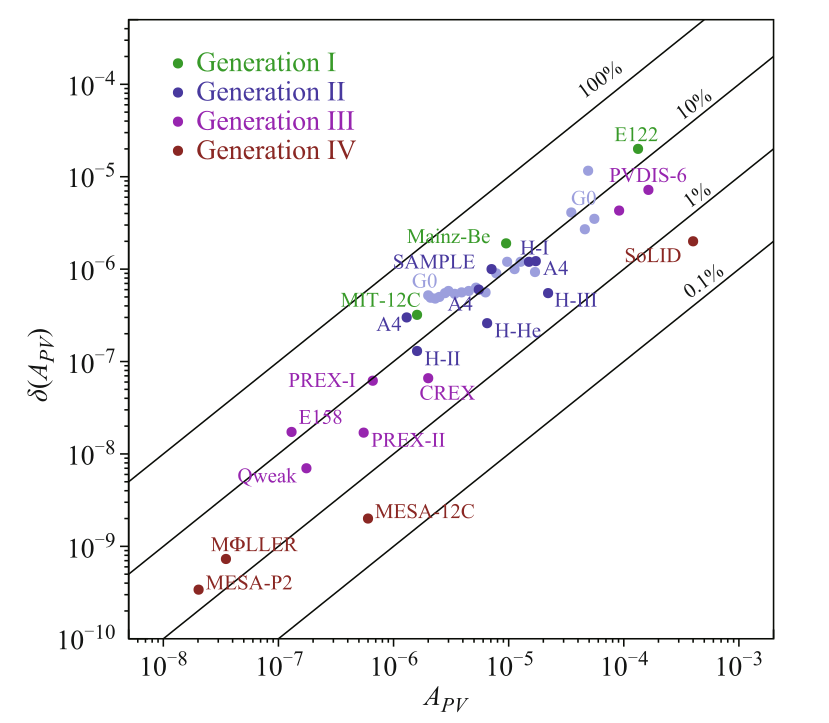
\includegraphics[width=0.5\linewidth]{PVES}
    \caption{Evolution of PVES experiments, solid lines represent the relative 
    precision. Generation I experiments (E122 (1978) \cite{PRESCOTT1978347}, 
    MIT-12C (1989) \cite{PhysRevLett.65.694} and Mainz-Be (1990) \cite{HEIL19891}) 
    did pioneering work to pave the way for PVES. Generation II experiments
    (the SAMPLE collaboration \cite{SAMPLE} at the MIT-Bates accelerator, 
    the G0 \cite{G0} and HAPPEX \cite{HAPPEX} collaboration at JLab and
    the A4 collaboration \cite{A4} at the Maizer Mikrotron (MAMI) accelerator) 
    were devoted to the exploration of strange FFs in nucleons.
    Generation III experiments (E158 at SLAC \cite{PhysRevLett.95.081601}, 
    Qweak \cite{PhysRevLett.111.141803} and PVDIS \cite{PhysRevLett.111.082501})
    tested the SM at low energy and measured the neutron skin thickness of nuclei
    (PREX-I/II and CREX). The planned Generation IV experiments (SoLID program \cite{SoLID}
    and MOLLER experiment \cite{Moller} at JLab, P2 experiment on the future
    Mainz Energy-recovery Superconducting Accelerator (MESA) \cite{MESA-P2})
    will continue to test the SM and explore the structure of nucleons with higher precision.
    (MESA-12C is the same experiment as MESA-P2 with a different \C target) }
\end{figure}
% precision of PREX-I doesn't allow to exclude many models, that's why people
% proposed PREX-II.

The idea of PVES experiments is very simple: scatter longitudinally polarized
electrons off unpolarized target (H, D, He, C, Ca, Pb etc.), then measure 
number of scattered electrons ($N$); reverse the beam helicity 
and do the same measurement. The PV asymmetry between different helicities will be:
\begin{equation}
    \CA_{PV} = \frac{N^+/I^+ - N^-/I^-}{N^+/I^+ + N^-/I^-}
\end{equation}
where $I$ is the beam current, and the superscript denote the beam helicity. 
Repeat the above procedure millions of times to get a statistically precise result
because the asymmetry is usually teeny tiny.

% low frequency noise and high frequency noise
% high energy ==> short wave length: 1 fm⁻¹ ~ 200 MeV
The devil is in the details.
Generally, PVES experiments require two experimental conditions: a high-energy polarized electron
beam and fast flipping of the beam polarization. Both requirements actually come to 
the same dependence: an intense source of polarized electrons with quick response. 
It took a few decades to develop such an electron source.
Right now, the electron source at JLab can reach a polarization of about 90\%,
continued efforts are being made to improve the polarization further.

The fast flipping requirement originates from the consideration to cancel various 
noises. To measure such a tiny quantity, it is essential to control
the experimental conditions as the same as possible between different
helicity states. One easy and effective method to meet such a requirement is fast 
flipping ($10^2 - 10^3$~Hz) of the beam helicity: the faster the helicity reversal, the smaller
the random noise in beam conditions, target density and other apparatus, the smaller
the introduced false asymmetry. This requirement makes PVES out of the capacity
of storage ring accelerators.

Though the fast reversal of the electron helicity, many efforts are still needed to
control the beam fluctuation, making it as small as possible. This is called
parity-quality beam (PQB). Possible systematic uncertainties in the source (injector) 
and accelerator will be controlled through the slow reversal of the beam helicity. 
In terms of the target deformity under electron bombardment,
a raster with very high scanning rate ($\sim$~kHz) will minimize this uncertainty. 
As for detection of scattered electrons, electron flux rather than single electron will
be counted due to high scattering rate ($\gtrsim$ MHz/$\mu$A) in such experiments.

The two sister experiments are conducted in Hall A at JLab. The CEBAF accelerator 
at JLab is one of the few facilities in the world that can do PVES experiments (
other facilities include MIMA and its successor MESA, the Facility for Antiproton
and Ion Research (FAIR) and the Facility for Rare Isotope Beams (FRIB)). CEBAF 
provided excellent polarized electron beams (helicity correlated difference at 
sub-nanometer level) to Hall A, with dedicated apparatus 
(polarimeter, target chamber, high resolution spectrometer (HRS) and others) in Hall A, 
we were able to measure this tiny PV asymmetry precisely.

% table of beam parameters
\begin{table}[h]
    \centering
    \begin{tabular}{l | c c }
	\hline
	&   PREX-II & CREX  \\
	\hline
	Target	& \Pb	& \Ca	\\
	Target Thickness (mm)	& 0.2554 + 0.5520 + 0.2566\tablefootnote{\Pb target composes of 3 foils: upstream Diamond + \Pb + downstream Diamond}    & 6	\\
	Target Density (g/cm${}^3$)   & 11.38 & 1.855	\\
	Number of Target & 10 & 1 + 1\tablefootnote{Only 1 was prepared for the experiment. After the target accident, a new one was prepared.}	\\ 
	Number of Used Target & 6 & 2	\\
	\hline
	Beam Energy (GeV) & 0.953 & 2.18  \\
	Beam Current ($\mu$A)	& 50-85	& 100-150   \\
	Average Beam Polarization (\%) & 89.7   & 87.1   \\
	Beam Bunch Rate (MHz)	& 499	& 499 \\
	Electrons/Bunch	($\times 10^6$)	& 1.75	& 3.76	\\  % FIXME for 70 and 150 uA
	Helicity Flip Rate (Hz) & 120/240   & 120   \\
	Power on the Target	& $\sim100$ W\@70~$\mu$A  & $\sim350$ W\@150~$\mu$A \\
	\hline
	Scattering Angle ($\deg$)   & 4.7	& 4.51 \\
	$Q^2$ ($\mathrm{GeV}^2$)	& 0.00616   & 0.0297	\\
	Scattering Rate (MHz/$\mu$A/arm)   & $\sim 30$\tablefootnote{This rate doesn't include the contribution from the diamond foils}   & $\sim0.2$ \\
	Scattering Rate (1/bunch/arm)   & $\sim 4.5$   & $\sim 0.05$ \\
	xsection (mbarn)    & 3930.6	& 5.3   \\
	Acceptance (msr)    &	0.0037 & 0.0037  \\
	\hline
	Collected Charge (C)	& 114	& 412	\\
	\hline
	Predicted $\CA_{pv}$ (ppm)	& 0.6   & 2 \\
	Proposed Precision  &	3\%   & 2.4\% \\
	Error on $R_n$ (fm)	& 0.05	& 0.02	\\
	\hline
    \end{tabular}
    \caption{Summary of experimental design and setup for PREX-II and CREX.}
    \label{tab:parameters}
% crex rate: https://logbooks.jlab.org/entry/3748863
\end{table}

%%%%%%%%%%%%%%%%%%%%%%%%%%%%%%%%%%%%%%%%%%%%%%%%%%%%%%%%%%%%%%%%%%%%%%%%
\section{Beam Parameters}
PREX-II and CREX are follow-up experiments to PREX-I, which also ran at JLab in 2010. 
With quite good control over the systematic uncertainty, but unfortunately, 
many technical challenges are encountered during the experiment, PREX-I's result is 
statistics-limited, achieving a precision of 10\% \cite{PhysRevLett.108.112502}:
$$ \CA_{Pb} = 656 \pm 60 \ (\text{stat}) \pm 14 \ (\text{syst}) \ \mathrm{parts-per-billion (ppb)} $$
Based on the experience and lessons learned from PREX-I, 
PREX-II and CREX have more well-established designs, which help to
meet the goal of high-precision.

One important feature of these two experiments is the redundancy design for critical
components: there are two slow helicity reversal systems for systematic uncertainty control,
two polarimeters for polarization measurement, multiple beam position
monitors (BPMs) and beam current monitors (BCMs) for beam parameter monitoring, 
multiple \Pb targets and finally two HRS for reception of the scattered electrons.

%%%%%%%%%%%%%%%%%%%%%%%%%%%%%%%%%%%%%%%%%%%%%%%%
\subsection{Uncertainty Budget}
The goal of PREX-II is to achieve the 1\% precision in the \Pb neutron radius proposed
by PREX-I, which requires the precision of PV asymmetry measurement better than 3\% \cite{PhysRevLett.106.252501}. 
CREX proposed a similar goal, that a precision of $0.02$~fm ($\sim 0.6\%$) in the
\Ca neutron radius will be an essential benchmark to test various microscopic 
models \cite{crex_proposal}, which correspond to a 2.4\% total uncertainty in PV asymmetry.

% page 7 in https://prex.jlab.org/DocDB/0000/000065/001/kutz_fom.pdf
As said above, PREX-I already has impressive control over systematic uncertainties (2.1\%),
so will the PREX-II and CREX. The main concern is to collect as much scattered 
electrons as possible to reduce statistical uncertainty, which is inversely 
proportional to $\sqrt{N}$, with $N$ being the total number of scattered electrons.
\begin{equation}
    \frac{\delta \CA}{\CA} = \sqrt{\sigma^2_{\text{stat}} + \sigma^2_{\text{sys}}}	
    \qquad 
    \sigma_{\text{stat}} = \frac{\sigma_{\text{det}}}{\CP\sqrt{N}}
\end{equation}
where $\sigma_{\text{det}}$ is the detector uncertainty and $\CP$ refers to the beam polarization.

\begin{table}[!h]
    \centering
    % page 19 in https://www.jlab.org/intralab/calendar/phys_seminar/2019/JLabtalk_20190206mod_Palatchi.pdf
    % Jinlon's slide says a 2% statistical uncertainty for CREX, while Caryn's slide says 4%
    % Paul's slide says 2.4%, maybe the total uncertainty
    \begin{tabular}{c| c c c}
	\hline
	Experiment  & PREX-I (\%)   & PREX-II (\%)	& CREX (\%)	\\
	\hline
	Charge Normalization	& 0.2	& 0.1	& 0.1	\\
	Beam Asymmetry		& 1.1	& 1.1	& 0.3	\\
	Detector Non-Linearity	& 1.2	& 1.0	& 0.3	\\
	Transverse Asymmetry	& 0.2	& 0.2	& 0.1	\\
	Polarization		& 1.3	& 1.1	& 0.8	\\
	Target Contamination	& 0.4	& 0.4	& 0.2	\\
	Inelastic Scattering	& $<0.1\%$  & $<0.1$    & 0.2   \\
	Effective $Q^2$		& 0.5	& 0.4	& 0.8	\\
	\hline
	Total Systematic	& 2.1	& 2	& 1.2	\\
	Statistical		& 9.1	& 2.2	& 2.1	\\
	\hline
	Total			& 9.2	& 3	& 2.4	\\
	\hline
    \end{tabular}
    \caption{Budget of systematic and statistical uncertainties in both experiments 
    \cite{prex-II_proposal, crex_proposal}
    }
\end{table}


%%%%%%%%%%%%%%%%%%%%%%%%%%%%%%%%%%%%%%%%%%%%%%%%
\subsection{Figure Of Merits (FOM)}
The choice of beam energy and scattering angle is a compromise of competing
factors. PV asymmetry prefers larger beam energy and larger scattering angle,
while scattering rate falls dramatically with beam energy and scattering angle.
$Q^2$ also likes smaller beam energy and scattering angle, and calculation 
shows that the sensitivity of PV asymmetry w.r.t. neutron radius is oscillating
along beam energy. All these considerations are incorporated into the FOM, which
is defined as:
\begin{equation}
    \text{FOM} = R \times \CA^2 \times \epsilon^2
\end{equation}
where R is the scattering rate, $\CA$ the PV asymmetry and $\epsilon$ 
the sensitivity of $\CA$ w.r.t. $R_n$. One difference here is that FOMs for most PVES 
experiments have only R and $\CA^2$, the inclusion of $\epsilon$ in our FOM helps
to achieve a higher precision in $R_n$ measurement.

%%%%%%%%%%%%%%%%%%%%%%%%
% from materials/rate_estimation.pdf
\subsubsection{Rate}
For a data set of N independent events sampled from one normal distribution 
$X\sim N(x_0, \sigma_0)$, the statistical uncertainty on the measured mean value
will be:
$$ \text{var}(\bar{x} = \frac{1}{n}\sum x_i) = \frac{1}{n^2}\text{var}(x_i) = \frac{\sigma_0^2}{n} 
\quad \Longrightarrow \sigma(\bar{x}) = \frac{\sigma_0}{\sqrt{n}} $$

Assume one want to measure a $1$~ppm asymmetry to 1\% statistical uncertainty,
\begin{equation}
    \frac{\sigma_\CA}{\CA} = \frac{1}{\CA}\frac{\sigma_{det}}{\sqrt{2N}} 
    \approx \frac{1}{\CA\sqrt{2N}} = 1\% \quad 
    \Longrightarrow N = 5 \times 10^{15} 
    \label{eq:statistical_error}
\end{equation}
a factor of 2 is included because there are two HRS arms.
One need to count $\sim10^{15}$ scattered electrons. Given a counting rate of 1~MHz, 
it will take $\frac{5\times 10^{15}}{1\ \mathrm{MHz}} = 5\times 10^{9}\ \mathrm{s} \approx 160$~years,
a completely unacceptable time scale. As a solution, the integrated flux technique is
adopted for a higher scattering rate, which is:
\begin{equation}
    \frac{dR(\theta)}{d\Omega} = \frac{d\sigma}{d\Omega}\ I\ t\ \frac{\rho}{A} \times N_A   
\end{equation}
\begin{itemize}
    \item $\frac{d\sigma}{d\Omega}$ is the fractional cross section in the unit of $\mathrm{cm}^2$/str.
    \item $I$ is the beam current in the unit of electrons/s.
    \item $t$ is the target thickness in the unit of cm.
    \item $\rho$ is the target density in the unit of g/cm${}^3$.
    \item $A$ is the atomic number.
    \item $N_A = 6.022\times 10^{23}$ is the Avogadro's constant.
\end{itemize}

The differential cross section is numerically calculated by our theoretical friends
with values of 3930.6~mbarn and 5.3~mbarn for \Pb and \Ca at their corresponding
kinematics. Other parameters can be checked out in Table~\ref{tab:parameters}.

The total rate will be the integration over the acceptance:
\begin{equation}
    R = \int \frac{dR(\theta)}{d\Omega} d\Omega = \frac{dR}{d\Omega} d\Omega
\end{equation}
PREX-II and CREX have an acceptance defined by the septum magnet and the Q1 collimator, 
which is $d\Omega = 0.0037$~str.

\begin{comment}
Finally, we should also consider radiative correction due to emission of virtual
and real soft photons (Bremsstrahlung radiation), and hard photons by vacuum polarization,
this correction is formulated as:
\begin{equation}
    \eta = \left(\frac{\Delta}{E} \right)^{bt}
\end{equation}
which is evaluated to be: $\eta \sim 0.5$.
\end{comment}

As shown in Fig.~\ref{fig:scattering_rate}, for both \Pb and \Ca, the scattering 
rate falls quickly along both the beam energy and the scattering angle, 
so one would like a small beam energy and a small scattering angle (equivalently
a small $\vec{q}$) for a large scattering rate.
\begin{figure}[!h]
    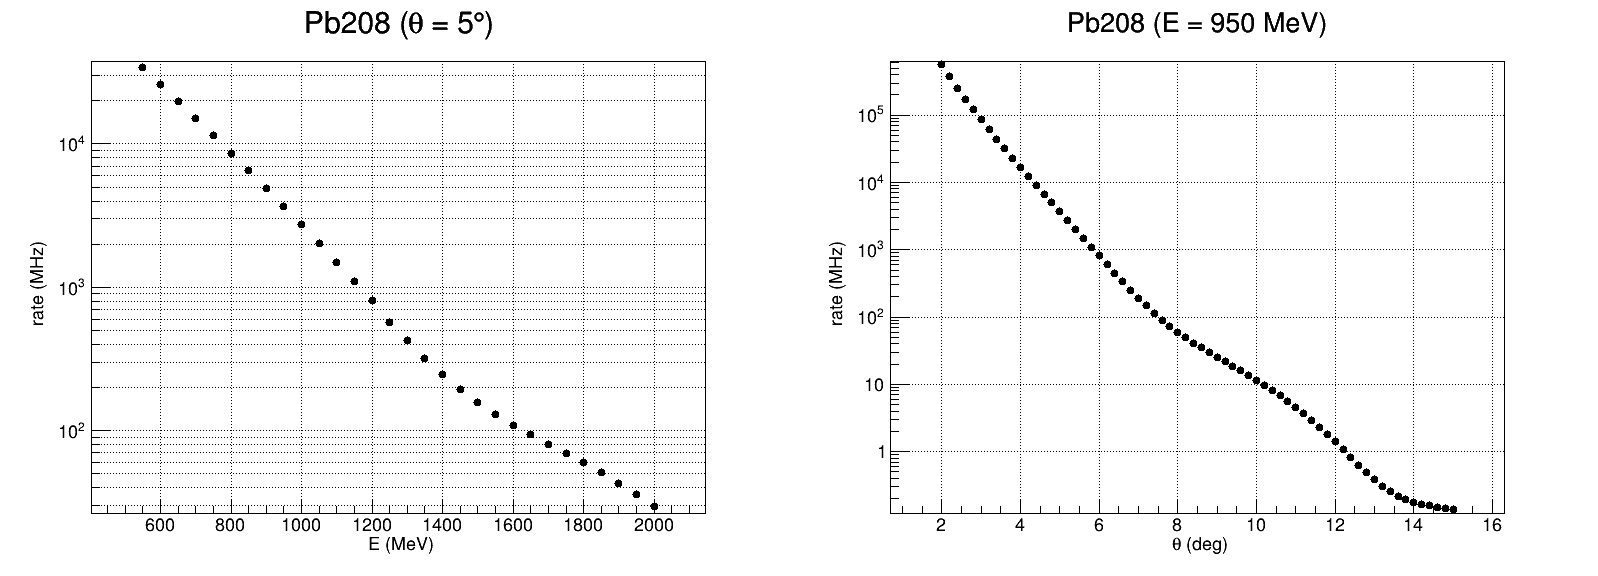
\includegraphics[width=0.5\linewidth]{Pb208_rate}
    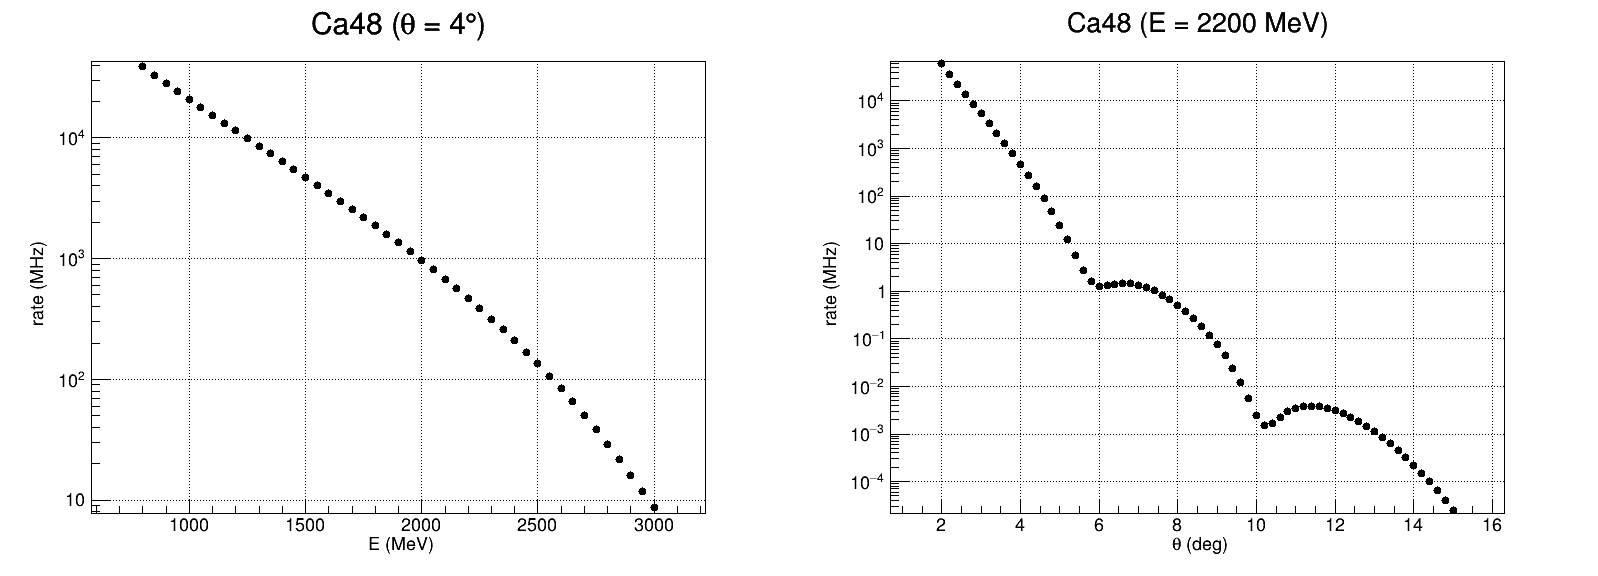
\includegraphics[width=0.5\linewidth]{Ca48_rate}
    \caption{Scattering rate versus the beam energy and the scattering angle for \Pb and \Ca,
    the other parameters (energy in the scattering angle plot and vice versa) 
    are fixed to their design values.}
    \label{fig:scattering_rate}
\end{figure}

%%%%%%%%%%%%%%%%%%%%%%%%
\subsubsection{Asymmetry and Sensitivity}
As shown in Eq.~\ref{eq:statistical_error}, the asymmetry itself matters,
a 2 times larger asymmetry means the run time can be reduced to one quarter,
a huge save of the beam time. So we should choose a kinematic region where
the asymmetry is large. Besides, asymmetry's sensitivity ($\epsilon$) to the neutron radius 
is also important. Keep in mind that our final goal is to extract the neutron radius
from the PV asymmetry, the more sensitive the asymmetry to the neutron radius, the
more precise the extracted neutron radius. The sensitivity is calculated
as the relative change of $\CA$ with 1\% change in the neutron radius.
\begin{equation}
    \epsilon = \frac{\delta \CA/\CA}{\delta R/R} = \frac{|\CA_{stretched} - \CA|/\CA}{1\%}
\end{equation}
Though asymmetry is what will be measured, one can estimate its value based
on some theoretical models, as is numerically calculated by our theoretical 
friends in \cite{PhysRevC.57.3430}.
\begin{figure}[!h]
    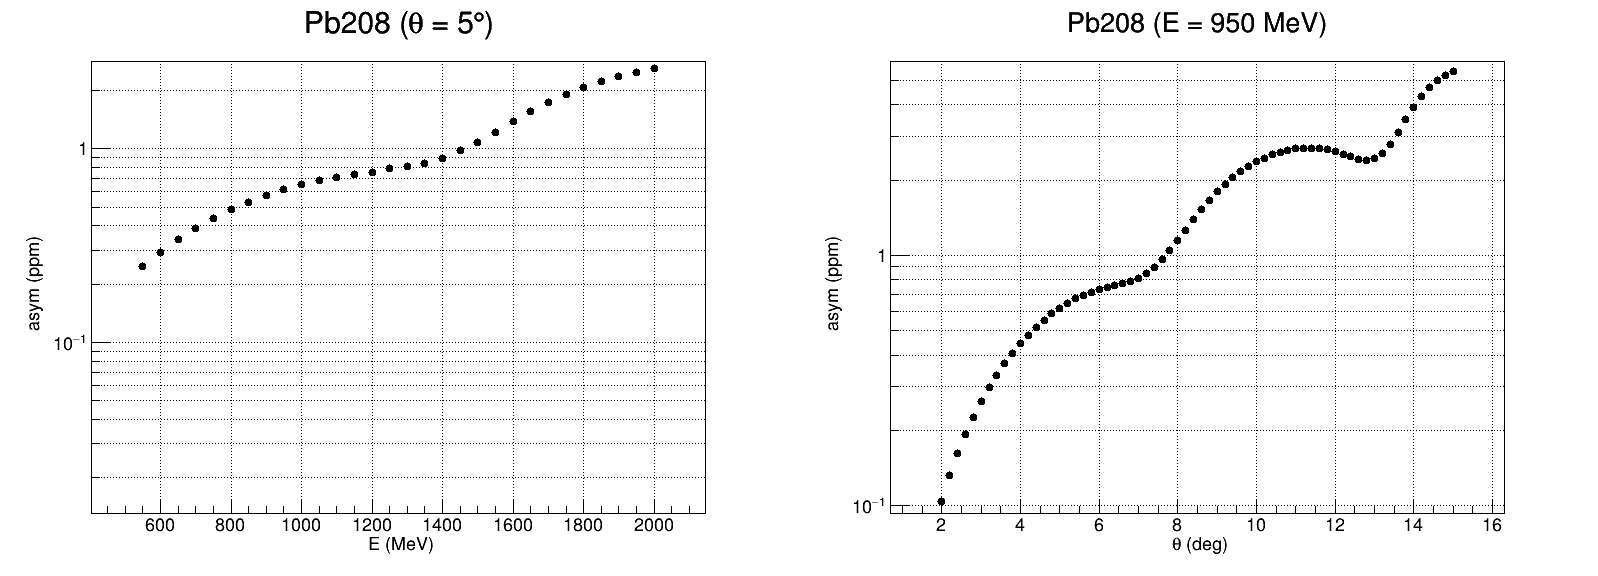
\includegraphics[width=0.5\linewidth]{Pb208_asym}
    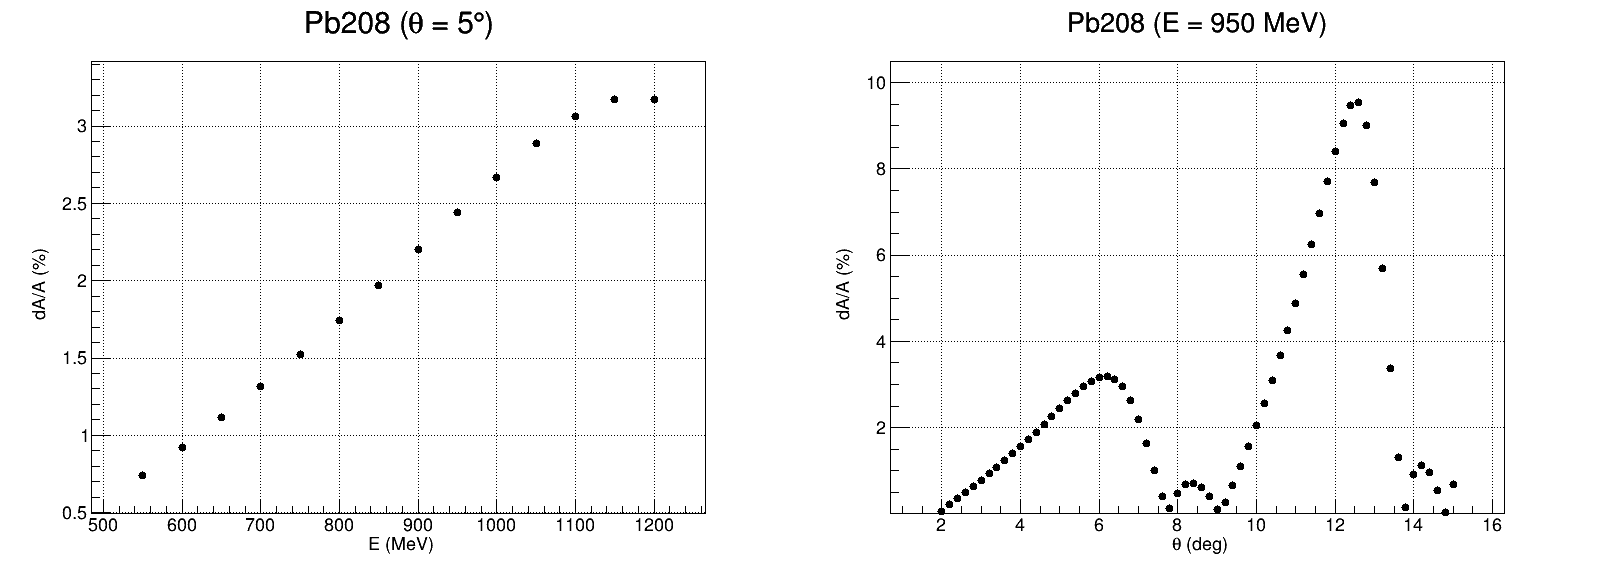
\includegraphics[width=0.5\linewidth]{Pb208_sen}
    \caption{Asymmetry and sensitivity plot for \Pb. The asymmetry increases along 
    the beam energy and goes upward with oscillation along the scattering angle. 
    The sensitivity also increases against the beam energy and oscillates against
    the scattering angle.  The sensitivity plot is calculated with 1\% change in 
    the neutron radius and it shows the absolute value.
    With $E$ = 950~MeV, there is a local maximum around $theta \sim 6^\circ$.
    }
\end{figure}
\begin{figure}[h!]
    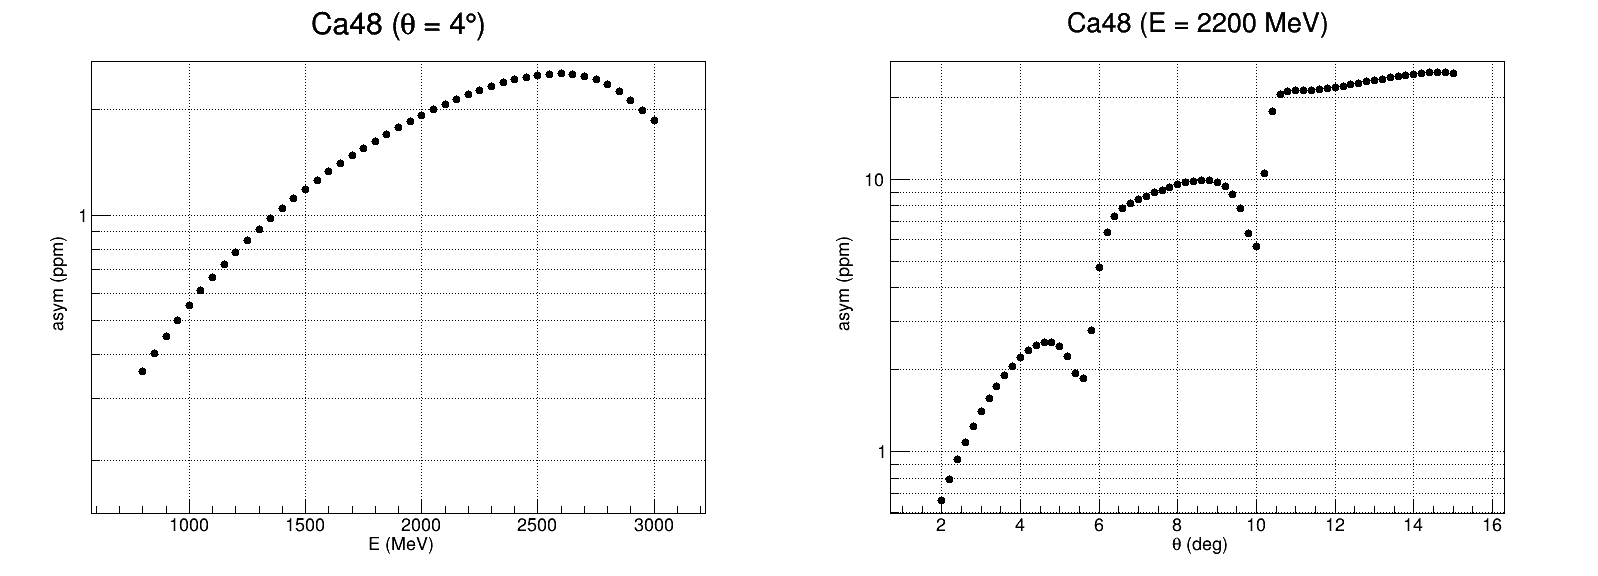
\includegraphics[width=0.5\linewidth]{Ca48_asym}
    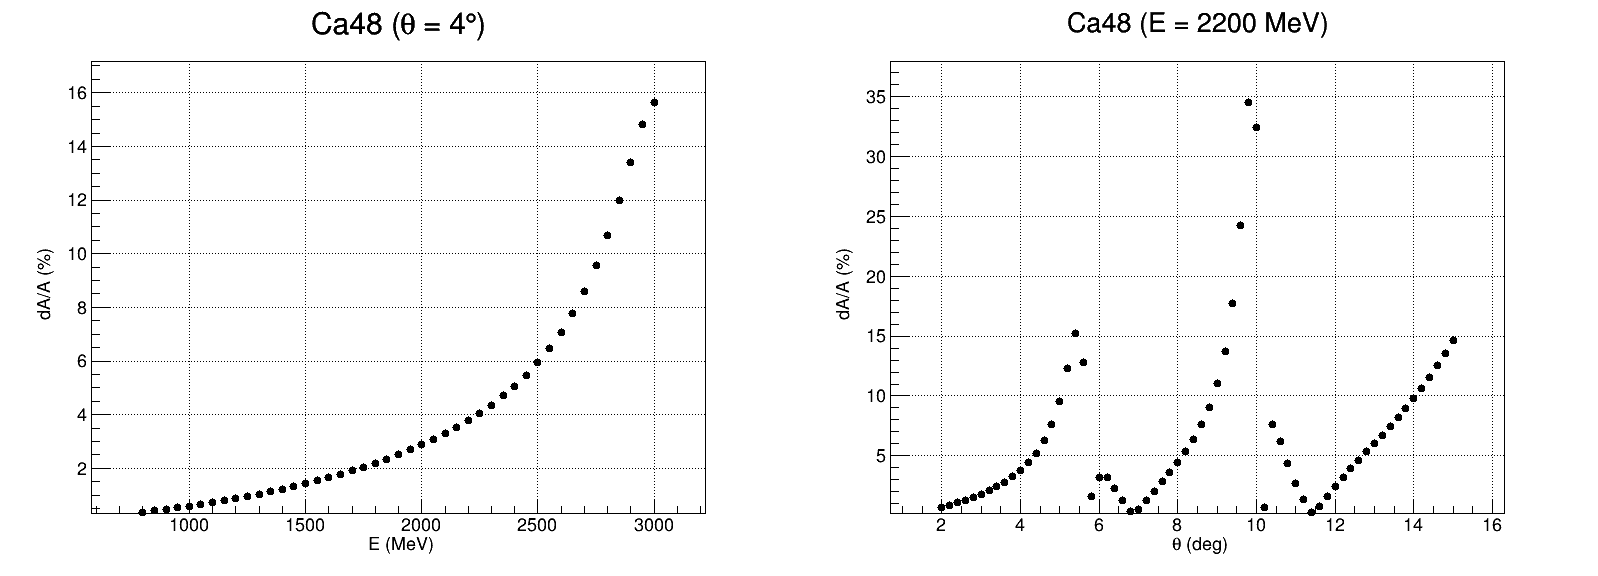
\includegraphics[width=0.5\linewidth]{Ca48_sen}
    \caption{Similar asymmetry and sensitivity plot for \Ca, the asymmetry maximize 
    around 2500~MeV with $\theta = 4^\circ$ and there is a local maximum 
    about $4.5^\circ$ when $E$ = 2200~MeV. As for the sensitivity, it increases
    monotonously along the beam energy and comes to a regional maximum around $5^\circ$
    with $E$ = 2200~MeV.
    }
    \label{fig:ca48_asym_sen}
\end{figure}

Based on the theoretical result, we can optimize the kinematics for both nuclei 
(consider only the statistical uncertainty here):
\begin{equation}
    \frac{\delta R}{R} = \frac{\delta \CA}{\CA} \frac{1}{\epsilon} 
	= \frac{\sigma_{det}}{\CP} \frac{1}{\sqrt{N} \CA \epsilon}
\end{equation}
To minimize $\delta R/R$, it is equivalent to maximize 
\begin{equation}
    \text{FOM} = N\times \CA^2 \times \epsilon^2
\end{equation}
\begin{figure}
    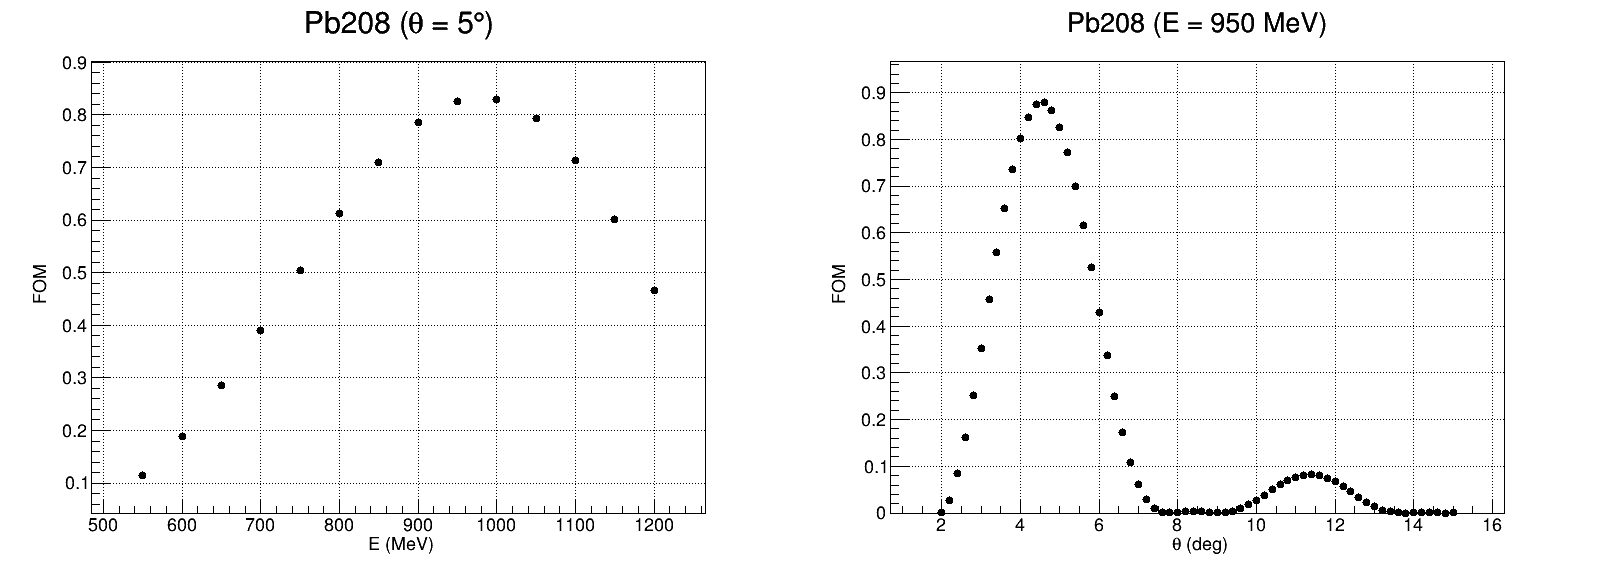
\includegraphics[width=0.5\linewidth]{Pb208_fom}
    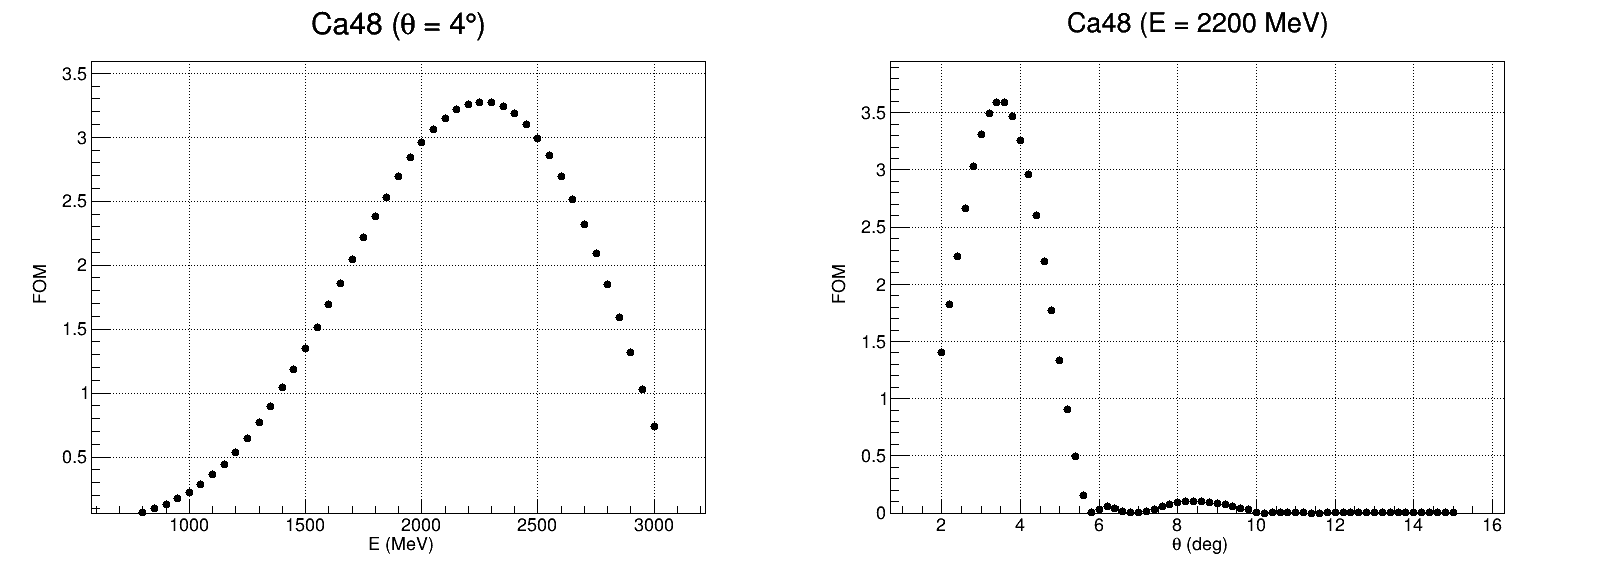
\includegraphics[width=0.5\linewidth]{Ca48_fom}
    \caption{For both nuclei, FOM supports a small scattering angle. As for the beam energy,
    FOM maximizes around 950 (2200)~MeV for \Pb (\Ca).}
\end{figure}

Given practical constraints on how low an angle ($4^\circ$) we can reach with 
septum magnets, the beam energy and the scattering angle were chosen to be 950 (2200)~MeV
and 5 (4)~degree for \Pb (\Ca). The beam energy of CREX is exactly a natural 1-pass beam
energy in CEBAF in the 12~GeV era.
\begin{comment}
For PREX-II: average sensitivity reduced by 5\% due to ${}^{12}C$ contamination
For CREX: average sensitivity reduced by 10\% due to ${}^{40}Ca$ contamination

% \subsubsection{Factor of 1.06}
While a quartz Cerenkov detector is valued for radiation hardness and insensitivity to soft backgrounds, there is a particular challenge for few GeV electrons. In this energy range, shower fluctuations in a thick or radiated detector significantly degrade energy resolution, while photon statistics degrade the energy resolution for a thin detector. The energy resolution $\Delta E$ at nominal electron energy E increases the statistical error that one would have with infinite resolution $\sigma_0$ to obtain the total statistical error:
$$ \sigma = \sigma_0\sqrt{1+\left(\frac{\Delta E}{E}\right)^2}$$
    
Based on experience in the PREX experiment, we expect an reduction of statistical precision of a factor of 1.06 due to detector resolution.
\end{comment}

%%%%%%%%%%%%%%%%%%%%%%%%%%%%%%%%%%%%%%%%%%%%%%%%
\subsection{Helicity Flip Frequency}
The main consideration for the choice of the 120~Hz (240~Hz) flip frequency 
was to cancel the 60 Hz power line noise, which is the major source of noise
in PVES experiments. 

There are a few methods to cancel this low frequency noise in a PVES experiment.
\begin{enumerate}
    \item Set the flip frequency to a very high value, say 1~kHz, then
	the change of fluctuations caused by this low frequency noise will be negligible
	between two nearby helicity windows and cancelled in the asymmetry calculation. 
	This methods can eliminate many low frequency noises and was adopted in the Qweak experiment.
    \item Integrate over this 60~Hz noise within a helicity window, which means
	$f = \frac{60}{n}\ \mathrm{Hz}\ (n = 1, 2, \cdots)$. This way no 60~Hz line noise
	will be recorded at all.
    \item Select a flip frequency of $f = n \times 60 \ \mathrm{Hz}$,
	then use helicity pattern to cancel the 60~Hz noise. For example, 
	if $f = 120$~Hz, then every $f/30 = 4$ continuous helicity windows form a 
	helicity pattern, asymmetry will be calculated based on helicity patterns. 
	This was used in PREX-II/CREX.
\end{enumerate}

In terms of cancelling the 60~Hz line noise, the second method works best,
it removes the line noise completely, while other two methods also cancel the noise
in their asymmetry calculation, it broadens the asymmetry width. But in a comprehensive
consideration, the frequency in the second method is not high enough to cancel
other low frequency noises. As for the first method, it is best in terms of % FIXME e.x. of other low frequency noises
removing low frequency noises, the only drawback is that with a fixed settle time $T_{\text{settle}}$
-- the time needed to settle a helicity state,
the higher the frequency, the lower the $T_{\text{stable}}$ -- the stable time window
during which we integrate scattered electrons, and therefore the longer the run time. 
As a compromise, the third method was chosen for PREX-II/CREX.

%%%%%%%%%%%%%%%%%%%%%%%%%%%%%%%%%%%%%%%%%%%%%%%%%%%%%%%%%%%%%%%%%%%%%%%%
\section{Continuous Electron Beam Accelerator Facility (CEBAF)}
\begin{figure}[h!]
    \begin{subfigure}[b]{0.59\textwidth}
    \begin{tikzpicture}
	\begin{scope}
	    \node[anchor=south west, inner sep=0] (image) at (0, 0)
	    { 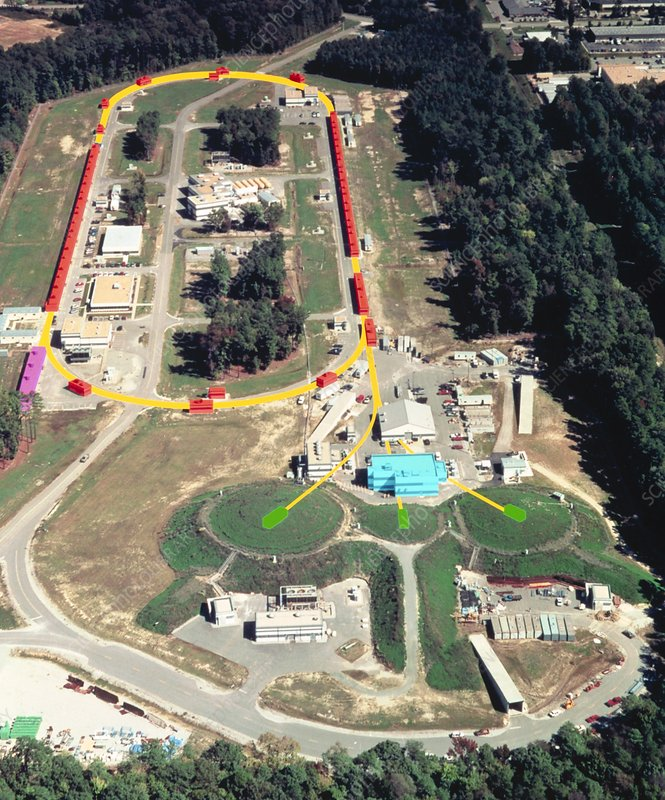
\includegraphics[width=\linewidth]{jlab.jpg} };
	    \begin{scope}[x={(image.south east)}, y={(image.north west)}]
		\node [red] at (0.415, 0.355) {\textbf{A}};
		\node [red] at (0.610, 0.355) {\textbf{B}};
		\node [red] at (0.780, 0.355) {\textbf{C}};
	    \end{scope}
	\end{scope}
    \end{tikzpicture}
    \end{subfigure}
    \begin{subfigure}[b]{0.5\textwidth}
	\includegraphics[width=0.9\linewidth]{tunnel_construction}
	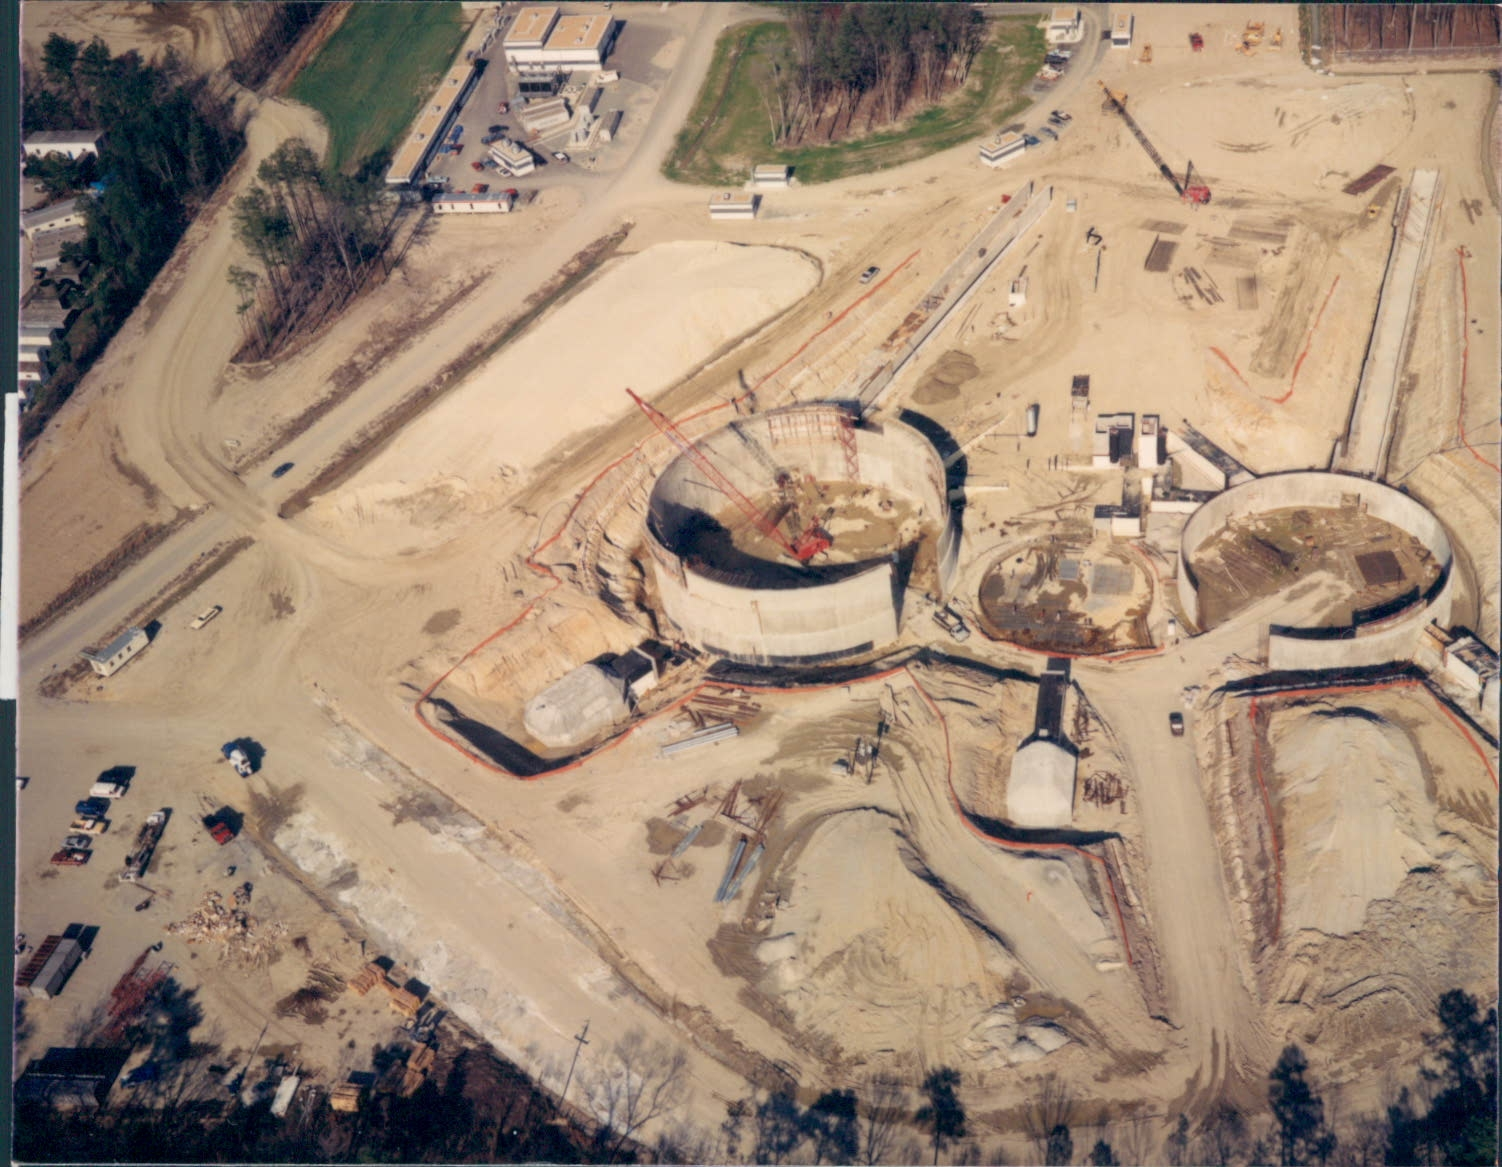
\includegraphics[width=0.9\linewidth]{hall_construction}
    \end{subfigure}

    \caption{Aerial view of JLab accelerator site, yellow line tells the position
    of the CEBAF accelerator and the three experimental halls are marked out as A/B/C 
    (Hall D locates on the top left corner, after the exit of the north LINAC).
    The accelerator tunnel is 30~feet ($\sim 9$~m) underground and 10~feet ($\sim 3$~m) 
    high, with a circumference of about 7/8~mile (1.4~km). There are two superconducting 
    LINACs (red lines), each of 1/4~mile (400~m). The pink part on the mid
    left is the location of injector. The right two plots show the tunnel and 
    experimental halls under construction.}
\end{figure}

\begin{figure}[h!]
    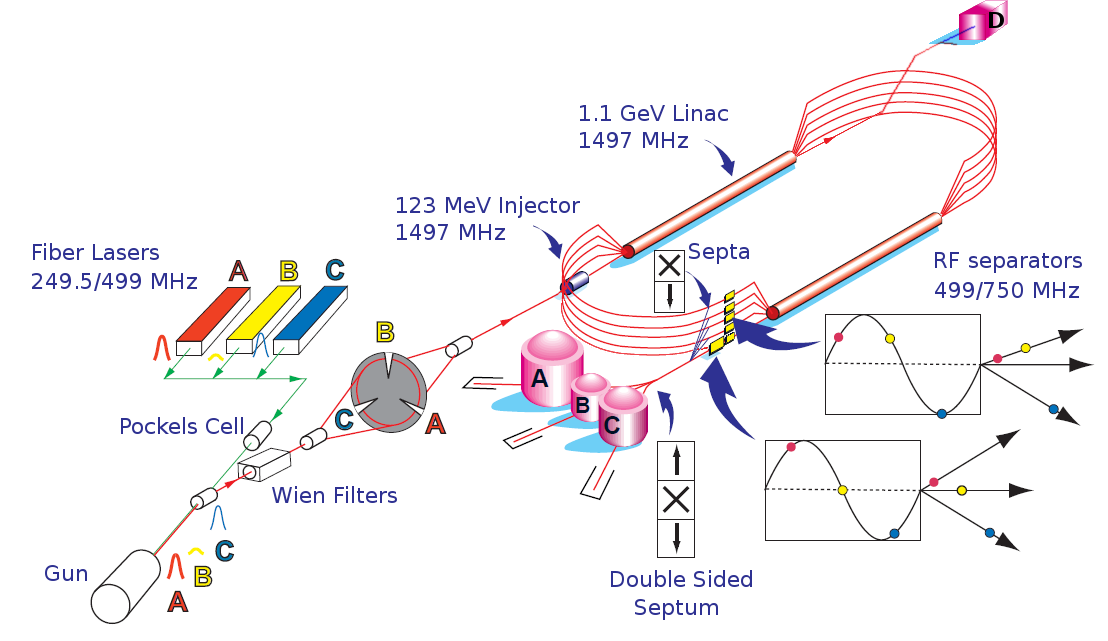
\includegraphics[width=0.9\linewidth]{cebaf.png}
    \caption{Schematic plot of CEBAF. The circular plate with three slits is the beam chopper,
    which has no slit for Hall D, that's why Hall D beams have to follow electron beams of other
    halls. During acceleration, low energy beams will be kicked into 
    higher arcs, while high energy beams will go through lower arcs. The magnetic
    field increases from higher arcs to lower arcs to keep electron trajectories
    have the same radii.}
    \label{fig:cebaf}
\end{figure}
CEBAF is able to deliver multi-GeV continuous wave (cw) electron beams of different
energies and different intensities to four experimental halls simultaneously.
With the 12~GeV upgrade, the injector energy is increased from 67.5~MeV to 
123~MeV. The north and south 1497~MHz linear accelerators (LINACs) each has 25 
superconducting radial frequency (SRF) cryomodules, capable of accelerating 
electrons at the peak rate of $1.1 \times 2 = 2.2$~GeV/turn. With 11 arcs of magnets
connecting the LINACs, Hall A, B and C can receive up
to $2.2 \times 5 = 11$~GeV cw beams. Hall D, with an extra half circle,
can receive up to 12~GeV cw beams. With this design, different nuclear 
experiments can be carried out in different halls without interfering each other,
theoretically.

As one can see in Fig.~\ref{fig:cebaf}, laser pulse ($\lambda = 780$~nm) from four lasers 
(Hall D laser is not shown in the plot) shoot in the electron gun 
(two electron guns in total) that 
operates at $-130$~kV to excite electrons, which interweaving with each other, 
forming a chain of electron bunches, with a phase difference of $120^\circ$ from 
nearby bunches (Hall D doesn't have its own slit in the chopper, therefore 
it follows either Hall A or Hall C). This electron chain is sent into the north LINAC
by the injector and accelerated by both LINACs. After reaching the desired energy,
they will be kicked out at the exit of the south LINAC and delivered to experimental
halls (A, B and C) for various experiments. 

The maximum beam current of $200\ \mu$A at (old) highest energy of 5~GeV 
available at CEBAF is limited by the rf power ($1\ \mathrm{MW} = 5\ \mathrm{GeV} \times 200\ \mu\mathrm{A}$) 
and by the beam power on the beam dump. While Hall B and D require only tiny 
amount of cw beams (at nA level), it is actually Hall A and C that consume 
almost all the electron beams, both can receive a few tenths to over one 
hundred $\mu$A cw beams.

While all four halls at JLab are dedicated to the study of nuclear structure, they
focus on different aspects. Hall A concentrates on form factors of various nuclei, 
Hall B digs into generalized parton distributions, Hall C devotes itself to precise
determination of valance quark properties in nuclei, and finally, the newly 
established Hall D explores origin of confinement through exotic mesons.
\begin{figure}[h!]
    \centering
    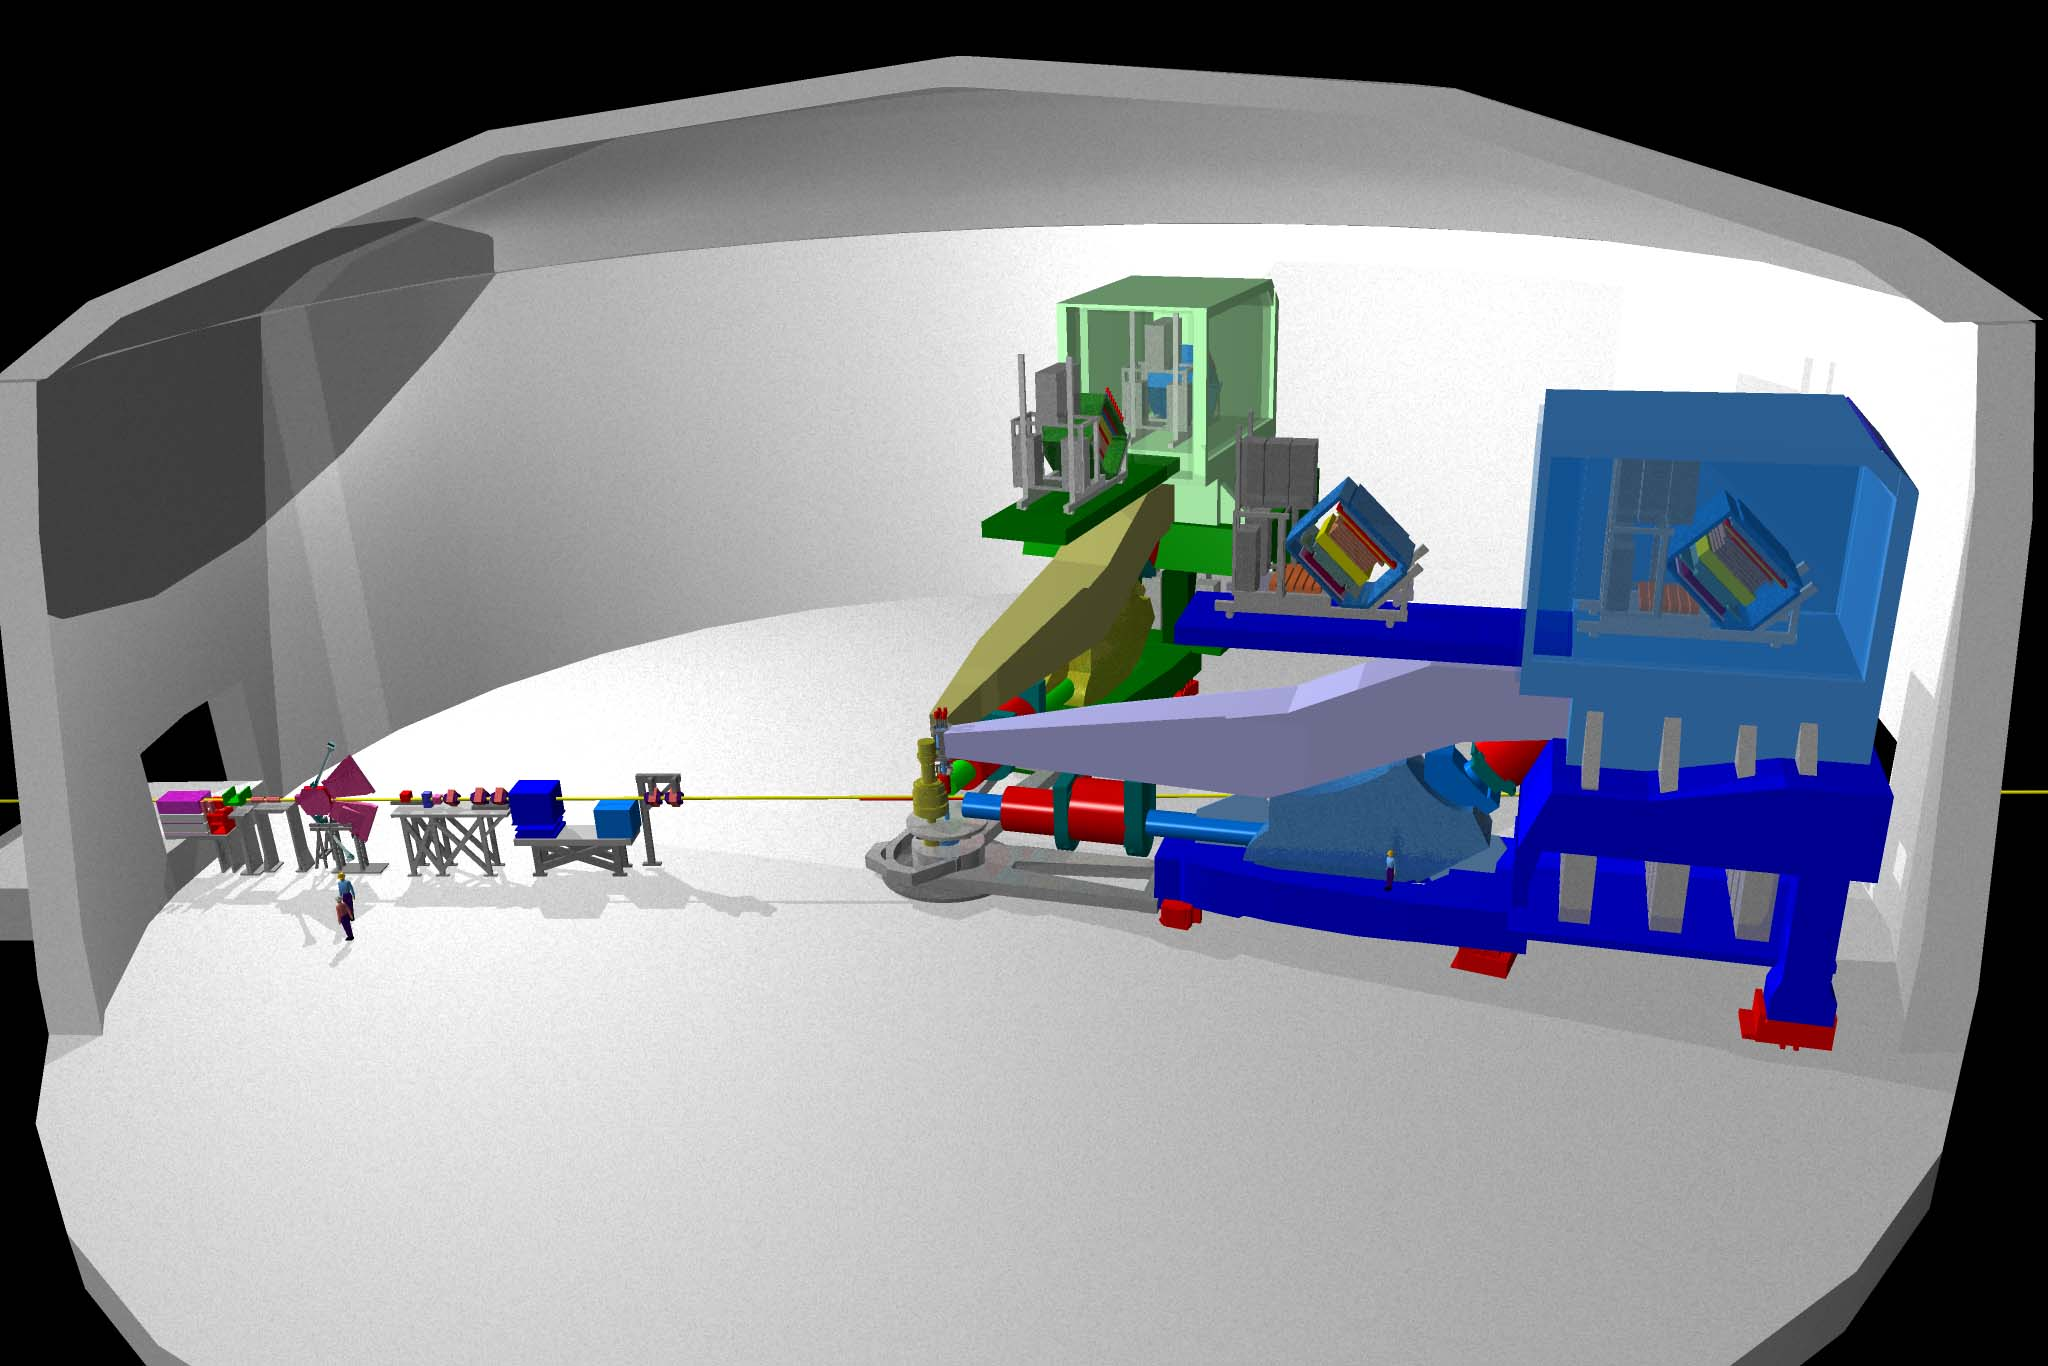
\includegraphics[width=0.48\linewidth]{hall_A}
    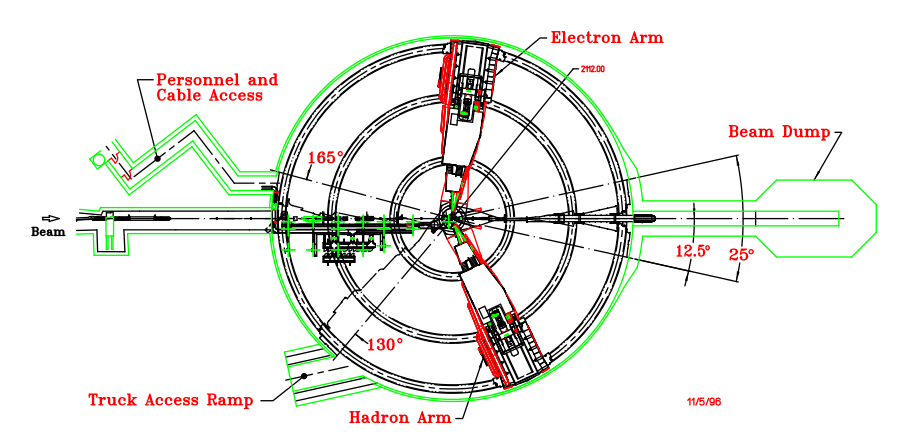
\includegraphics[width=0.51\linewidth]{hall_A_bird}
    \caption{3D and bird view of Hall A \cite{halla_manual}. Originally, the 2 spectrometers
    were called High Resolution Hadron Spectrometer (HRHS) and High Resolution Electron
    Spectrometer (HRES), but they are essentially identical to each other and
    can be used interchangeably.
    so now they are called left arm (HRS-L) and right arm HRS (HRS-R).
    }
\end{figure}

Because all four halls shared the same electron source and the same accelerator, 
cooperation is needed to make them work at the same time. In terms of the electron
source, PVES experiments usually have priority over other experiments to maintain 
quality of the polarized electron beam. As for the LINACs, if one hall wants
a smaller energy, say 1~GeV, then the LINAC power will be reduced to 1~GeV/turn,
which will be applied to other electron beams, therefore limiting the 
highest energy available in other halls. Careful schedule is needed to make sure
every hall gets what they want.
%%%%%%%%%%%%%%%%%%%%%%%%%%%%%%%%%%%%%%%%%%%%%%%%%%%%%%%%%%%%%%%%%%%%%%%%
\section{Polarized Electron Beam}
% The key to the success of this experiment was the 1975 discovery of a new method for producing
% polarized electrons made by a group in Colorado, which included E.L. Garwin of SLAC.
% Shortly thereafter, a new source was built for the SLAC linac utilizing the method, thus
% allowing for the 1978 parity violation measurements which were in close agreement with
% those predicted by the GWS model. 

%%%%%%%%%%%%%%%%%%%%%%%%%%%%%%%%%%%%%%%%%%%%%%%%
\subsection{Polarized Electron Source}
PVES experiments motivate the development of the polarized electron source, which 
is required to produce stable high-polarization electron beams at a wide range of intensity, 
from nA to A depending on the experiment. The source should be capable of rapid helicity
reversal ($\sim 100-1000$~Hz) with negligible impact on other properties of the electron beam.

Currently, GaAs-based semiconductor photoemission source is % confirmed by Wang Yan
the only choice on the market that can be used as the polarized electron source.
Historically, this kind of electron source was the only one that could satisfy high peak 
currents required by the low duty factors of the old accelerators and rapid helicity 
reversal required by PVES experiments. That's why it is the only player on the market now.
Over the past few decades, pulsed beam has been replaced by continuous beam while
this electron source is inherited and further developed. The polarized electron
source used by CEBAF can produce electron beams with polarization greater than
85\%, much larger than the 37\% polarization from its inauguration at SLAC. \cite{PRESCOTT1978347}

The design was first proposed independently by Garwin, Pierce and Siegmann \cite{GARWIN}
and by Lampel and Weisbuch \cite{LAMPEL1975877}. The idea is straightforward:
when circularly polarized laser light with carefully selected energy 
$E_{\text{gap}} < h\nu < E_{\text{gap}} + \Delta$
shoot on the semiconductor, only electrons on the valance band $P_{3/2}$ will be
pumped into the conduction band $S_{1/2}$. The selection rule makes sure only
those transitions that satisfy $\Delta m_j = +1 \ (-1)$ can occur for circularly
right (left) incoming photons, as shown in Fig.~\ref{fig:excitation}.
The ratio of the transition rate is also marked out in circle in the plot, 
which can be calculated from the Clebsch-Gordan coefficient easily. % FIXEM reference
The excited electrons are polarized and different states have different pumping rate, 
in this way, polarized electron beam is produced, with a polarization of: $\CP$ = (3-1)/(3+1) = 50\%,
for both helicities.
\begin{figure}[!h]
    \tikzmath{\yone=1.3; \ytwo=2.5; \ythree=5;} 
    \centering
    \begin{subfigure}[b]{0.49\textwidth}
	\centering
	\begin{tikzpicture}
	    \centering
	    \begin{axis}[axis lines=middle,
		xmin=-1.4, xmax=2.75,
		ymin=0, ymax=7,
		xlabel={\large $k$},
		ylabel={\large$E$},
		xlabel style={below},
		xtick=\empty,
		ytick=\empty,
		x axis line style={draw=none},
		% clip=false,
		]
		\addplot[Violet, line width=3pt, samples=100, domain=-0.7:0.7, name path=A] {-2*x^2 + \yone};
		\addplot[OliveGreen, line width=3pt, samples=100, domain=-0.7:0.7, name path=B] {-2*x^2 + \ytwo};
		\addplot[OliveGreen, line width=3pt, samples=100, domain=-0.7:0.7, name path=B] {-1.2*x^2 + \ytwo};
		\addplot[Blue, line width=3pt, samples=100, domain=-0.7:0.7, name path=B] {2*x^2 + \ythree};
		\draw [/pgfplots/every inner x axis line, draw=black] (0,0) -- (\pgfkeysvalueof{/pgfplots/xmax}, 0); 
		\draw [dashed, draw=black] (0,\yone) -- (\pgfkeysvalueof{/pgfplots/xmax}, \yone);
		\draw [dashed, draw=black] (0,\ytwo) -- (\pgfkeysvalueof{/pgfplots/xmax}, \ytwo);
		\draw [dashed, draw=black] (0,\ythree) -- (\pgfkeysvalueof{/pgfplots/xmax}, \ythree);
		\draw [stealth-stealth, thick] (0.8, \yone) -- (0.8, \ytwo) node [midway, right] {\bm{$\Delta = 0.34\ \mathrm{eV}$}};
		\draw [stealth-stealth, thick] (0.8, \ytwo) -- (0.8, \ythree) node [midway, right] {\bm{$E_{\text{gap}} = 1.42\ \mathrm{eV}$}};
		\node [Violet, below] at (-1, \yone) {\large\bm{$P_{1/2}$}};
		\node [OliveGreen, below] at (-1, \ytwo) {\large\bm{$P_{3/2}$}};
		\node [Blue, above] at (-1, \ythree) {\large\bm{$S_{1/2}$}};
		\node [left, above] at (-0.2, \ytwo) {\large\bm{$E_F$}};
	    \end{axis}
	\end{tikzpicture}
    \end{subfigure}
    \hfill
    \begin{subfigure}[b]{0.49\textwidth}
	\centering
	\begin{tikzpicture}
	    \begin{axis}[axis lines=middle,
		xmin=0, xmax=8,
		ymin=0, ymax=7,
		xlabel={\large $m_j$},
		ylabel={\large$E$},
		xlabel style={below},
		xtick=\empty,
		ytick=\empty,
		]
		\draw [/pgfplots/every inner y axis line, draw=black] (6.5,0) -- (6.5, \pgfkeysvalueof{/pgfplots/ymax}) node [below right] {\large J}; 
		\draw [draw=Violet, line width=2pt] (1.25,\yone) -- (2.25, \yone) node [midway, below, Violet] {\textbf{-1/2}};
		\draw [draw=Violet, line width=2pt] (4.25,\yone) -- (5.25, \yone) node [midway, below, Violet] {\textbf{+1/2}};
		\draw [draw=OliveGreen, line width=2pt] (0.5,\ytwo) -- (1.5, \ytwo) node [midway, below, OliveGreen] {\textbf{-3/2}};
		\draw [draw=OliveGreen, line width=2pt] (2,\ytwo) -- (3, \ytwo) node [midway, below, OliveGreen] {\textbf{-1/2}};
		\draw [draw=OliveGreen, line width=2pt] (3.5,\ytwo) -- (4.5, \ytwo) node [midway, below, OliveGreen] {\textbf{+1/2}};
		\draw [draw=OliveGreen, line width=2pt] (5,\ytwo) -- (6, \ytwo) node [midway, below, OliveGreen] {\textbf{+3/2}};
		\draw [draw=Blue, line width=2pt] (2,\ythree) -- (3, \ythree) node [midway, above, Blue] {\textbf{-1/2}};
		\draw [draw=Blue, line width=2pt] (3.5,\ythree) -- (4.5, \ythree) node [midway, above, Blue] {\textbf{+1/2}};
		\node [Violet, right] at (6.7, \yone-0.1) {\large\bm{$P_{1/2}$}};
		\node [OliveGreen, right] at (6.7, \ytwo-0.1) {\large\bm{$P_{3/2}$}};
		\node [Blue, right] at (6.7, \ythree-0.1) {\large\bm{$S_{1/2}$}};

		\draw [-stealth, Red, line width=2pt] (1, \ytwo) -- (2.5, \ythree) node [midway, circle, fill=CornflowerBlue, text=Black] {\textbf{3}};
		\draw [-stealth, Red, line width=2pt] (2.5, \ytwo) -- (4, \ythree);
		\node [above, Red] at (1, \ytwo+0.5) {\bm{$\sigma^+$}};
		\draw [-stealth, YellowOrange, line width=2pt] (4, \ytwo) -- (2.5, \ythree) node [midway, circle, fill=CornflowerBlue, text=Black] {\textbf{1}};
		\draw [-stealth, YellowOrange, line width=2pt] (5.5, \ytwo) -- (4, \ythree) node [midway, circle, fill=CornflowerBlue, text=Black] {\textbf{3}};
		\node [above, YellowOrange] at (5.5, \ytwo+0.5) {\bm{$\sigma^-$}};
	    \end{axis}
	\end{tikzpicture}
    \end{subfigure}
    \caption{Excitation of electrons in the semiconductor. Excited electrons with $J_z =$ +1/2 (-1/2) are right (left)-handed.}
    \label{fig:excitation}
\end{figure}

\begin{figure}[!h]
    \centering
    \begin{subfigure}[b]{0.32\textwidth}
	\tikzmath{\yone=2.5; \ytwo=5; \ythree=9.5;} 
	\centering
	\resizebox{\textwidth}{0.33\textheight}{
	\begin{tikzpicture}
	    \centering
	    \begin{axis}[
		axis lines=middle,
		xmin=-3, xmax=1,
		ymin=0, ymax=10,
		hide axis,
		]
		\draw [dashed] (\pgfkeysvalueof{/pgfplots/xmin}, \yone) -- (0, \yone) node [right] {\bm{$E_F$}};
		\draw [dashed] (\pgfkeysvalueof{/pgfplots/xmin}, \ytwo) -- (0, \ytwo);
		\draw [dashed] (\pgfkeysvalueof{/pgfplots/xmin}, \ythree) -- (0, \ythree);
		\draw [Violet, line width=2pt] (0, 0) -- (0, \ythree) -- (\pgfkeysvalueof{/pgfplots/xmax}/4, \ythree) node [right, Black] {\bm{$E_\infty$}};
		\fill [pattern=north east lines] (\pgfkeysvalueof{/pgfplots/xmin}, \yone)  -- (-1, \yone) arc (90:0:1) -- (0, 0) -- (\pgfkeysvalueof{/pgfplots/xmin}, 0) -- (\pgfkeysvalueof{/pgfplots/xmin}, \yone);
		\draw [Violet, line width=2pt] (\pgfkeysvalueof{/pgfplots/xmin}, \yone)  -- (-1, \yone) arc (90:0:1);
		\draw [Violet, line width=2pt] (\pgfkeysvalueof{/pgfplots/xmin}, \ytwo)  -- (-1, \ytwo) arc (90:0:1);
		\draw [stealth-stealth, thick] (\pgfkeysvalueof{/pgfplots/xmin} + 0.8, \yone) -- (\pgfkeysvalueof{/pgfplots/xmin} + 0.8, \ytwo) node [midway, left] {\bm{$E_{\text{gap}}$}};
		\draw [stealth-stealth, thick, Red] (-0.5, \ytwo) -- (-0.5, \ythree) node [midway, left] {\textbf{PEA = 4.07~eV}};
		\node [Red, above] at (\pgfkeysvalueof{/pgfplots/xmin}/2, 0) {\textbf{GaAs}};
		\node [Red, above right] at (0, 0) {\textbf{Vac}};
		\node [below left, text width=2cm] at (-0.5, \yone) {\textbf{Valance Band}};
		\node [below left, text width=2cm] at (-0.5, \ytwo) {\textbf{Conduction Band}};
	    \end{axis}
	\end{tikzpicture}
	}
	\label{fig:PEA}
    \end{subfigure}
    \hfill
    \begin{subfigure}[b]{0.32\textwidth}
	\tikzmath{\yone=2.5; \ytwo=5; \ythree=9.5;} 
	\centering
	\resizebox{\textwidth}{0.33\textheight}{
	\begin{tikzpicture}
	    \centering
	    \begin{axis}[
		axis lines=middle,
		xmin=-3, xmax=1,
		ymin=0, ymax=10,
		hide axis,
		]
		\draw [dashed] (\pgfkeysvalueof{/pgfplots/xmin}, \yone) -- (0, \yone) node [right] {\bm{$E_F$}};
		\draw [dashed] (\pgfkeysvalueof{/pgfplots/xmin}, \ytwo) -- (0, \ytwo);
		\node at (0, \pgfkeysvalueof{/pgfplots/ymax}) {};
		\draw [OliveGreen, line width=5pt] (-0.07, 0) -- (-0.07, \ytwo);
		\draw [Violet, line width=2pt] (0, 0) -- (0, \ytwo) -- (\pgfkeysvalueof{/pgfplots/xmax}/4, \ytwo) node [right, Black] {\bm{$E_\infty$}};
		\fill [pattern=north east lines] (\pgfkeysvalueof{/pgfplots/xmin}, \yone)  -- (-1, \yone) arc (90:0:1) -- (0, 0) -- (\pgfkeysvalueof{/pgfplots/xmin}, 0) -- (\pgfkeysvalueof{/pgfplots/xmin}, \yone);
		\draw [Violet, line width=2pt] (\pgfkeysvalueof{/pgfplots/xmin}, \yone)  -- (-1, \yone) arc (90:0:1);
		\draw [Violet, line width=2pt] (\pgfkeysvalueof{/pgfplots/xmin}, \ytwo)  -- (-1, \ytwo) arc (90:0:1);
		\node [Red, above] at (\pgfkeysvalueof{/pgfplots/xmin}/2, 0) {\textbf{GaAs}};
		\node [Red, above] at (-0.03, 0) {\textbf{Cs}};
		\node [Red, above right] at (0.1, 0) {\textbf{Vac}};
	    \end{axis}
	\end{tikzpicture}
	}
	\label{fig:ZEA}	% zero EA
    \end{subfigure}
    \hfill
    \begin{subfigure}[b]{0.32\textwidth}
	\tikzmath{\yone=2.5; \ytwo=5; \ythree=4; \surface=0.8;} 
	\centering
	\resizebox{\textwidth}{0.33\textheight}{
	\begin{tikzpicture}
	    \centering
	    \begin{axis}[
		axis lines=middle,
		xmin=-3, xmax=1,
		ymin=0, ymax=10,
		hide axis,
		]
		\draw [dashed] (\pgfkeysvalueof{/pgfplots/xmin}, \yone) -- (0, \yone) node [right] {\bm{$E_F$}};
		\draw [dashed] (\pgfkeysvalueof{/pgfplots/xmin}, \ytwo) -- (0, \ytwo);
		\draw [dashed] (\pgfkeysvalueof{/pgfplots/xmin}, \ythree) -- (0, \ythree);
		\node at (0, \pgfkeysvalueof{/pgfplots/ymax}) {};
		\draw [Violet, line width=2pt] (0, 0) -- (0, \ythree) -- (\pgfkeysvalueof{/pgfplots/xmax}/4, \ythree) node [right, Black] {\bm{$E_\infty$}};
		\fill [pattern=north east lines] (\pgfkeysvalueof{/pgfplots/xmin}, \yone)  -- (-1-\surface, \yone) arc (90:0:1) -- (-\surface, 1.4) arc (180:270:\surface) --  (0, 0) -- (\pgfkeysvalueof{/pgfplots/xmin}, 0) -- (\pgfkeysvalueof{/pgfplots/xmin}, \yone);
		\draw [Violet, line width=2pt] (-\surface, 0) -- (-\surface, \ytwo/2 + \ythree/2) arc (180:270:\surface);
		\draw [Violet, line width=2pt] (-\surface, 1.4) arc (180:270:\surface);
		\draw [Violet, line width=2pt] (\pgfkeysvalueof{/pgfplots/xmin}, \yone)  -- (-1-\surface, \yone) arc (90:0:1);
		\draw [Violet, line width=2pt] (\pgfkeysvalueof{/pgfplots/xmin}, \ytwo)  -- (-1-\surface, \ytwo) arc (90:0:1);
		\node [Red, above] at (\pgfkeysvalueof{/pgfplots/xmin}/2, 0) {\textbf{GaAs}};
		\node [Red, above] at (-0.4, 0) {\bm{$Cs_2O$}};
		\node [Red, above right] at (0.1, 0) {\textbf{Vac}};

		\node (e1) at (\pgfkeysvalueof{/pgfplots/xmin}/5*3, \yone)[circle, fill=CornflowerBlue, text=Black] {\textbf{e}};
		\node (e2) at (\pgfkeysvalueof{/pgfplots/xmin}/5*3, \ytwo)[circle, fill=CornflowerBlue, text=Black] {\textbf{e}};
		\node (e3) at (0.2, \ythree*1.1)[circle, fill=CornflowerBlue, text=Black] {\textbf{e}};
		\draw [-stealth, thick, CornflowerBlue] (e1) -- (e2);
		\draw [-stealth, thick, CornflowerBlue] (e2) -- (e3);
		\draw [stealth-stealth, thick, Red] (-2.2, \ytwo) -- (-2.2, \ythree) node [midway, left] {\textbf{NEA}};
	    \end{axis}
	\end{tikzpicture}
	}
	\label{fig:NEA}
    \end{subfigure}
    \caption{The energy band diagram of GaAs near its surface. 
    Left: bare p-type GaAs, the large positive electron affinity (PEA) 
    prevents electrons from escaping the surface; 
    Middle: p-type GaAs with a cesiated surface, the electron affinity (EA)
    is 0, but electrons still can't escape the surface easily; 
    Right: GaAs with layer of cesium oxide; the electron vacuum energy $E_\infty$ is
    lowered to make a negative EA so that electrons can break free from the surface
    easily. \cite{CARDMAN1992317}}
    \label{fig:electron_affinity}
\end{figure}
The next challenge is to liberate the polarzied electrons from the material, without 
degenerating the polarization significantly. As shown in Fig.~\ref{fig:electron_affinity},
for bare GaAs, a 4.07~eV electron affinity (EA) prevents any electrons from
leaving the surface. To solve this problem, a condition known as negative
electron affinity (NEA) is used, that is to make the energy of the electron in 
the vacuum just outside the surface lower than the conduction band energy by
adding a layer a cesium oxide on the surface of a pure GaAs semiconductor.

By the NEA technique, one is able to get polarized electron beams, but never
reach the ideal 50\% polarization: achieved polarization ranges between 25 to 43\%. 
The polarization loss is due to spin dilution as electrons diffuse to the 
semiconductor surface. From this aspect, one can increase the polarization by 
reducing the thickness of the GaAs crystal. However, even the thinnest
GaAs crystal can't give a polarization greater than 50\%. New strategies 
are needed. The answer is the strained GaAs \cite{CARDMAN1992317}.

With a strained layer, the degeneracy of the $P_{3/2}$ state is split, 
only states with $m_j = \pm 3/2$ will be pumped, therefore reaching a
100\% polarization, in ideal case. The real polarization achieved by the CEBAF electron
source is about 88\%.
\begin{figure}[h!]
    \tikzmath{\yone=1.3; \ytwo=2.5; \ythree=5;} 
    \centering
    \begin{subfigure}[b]{0.49\textwidth}
	\centering
	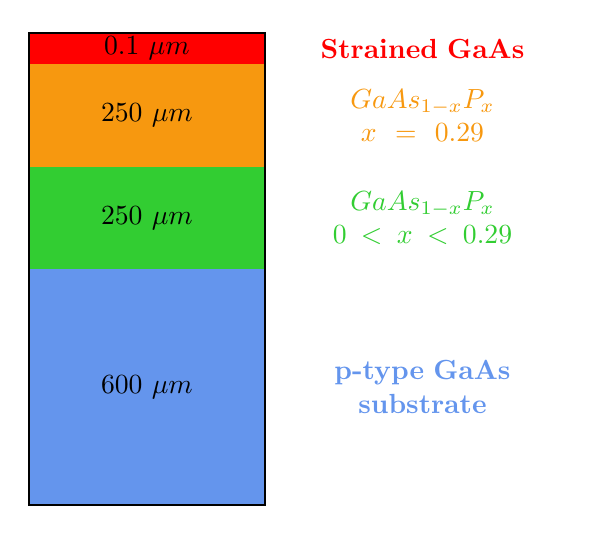
\begin{tikzpicture}
	    \tikzstyle{explain} = [align=center] 
	    \centering
	    \fill [CornflowerBlue] (0, 0) rectangle (3, 3);
	    \node at (3/2, 3/2) {\bm{$600 \ \mu m$}};
	    \node [explain, CornflowerBlue, text width=3.4 cm] at (5, 3/2) {\textbf{p-type GaAs substrate}};
	    \fill [LimeGreen] (0, 3) rectangle (3, 3+1.3);
	    \node at (3/2, 3 + 1.3/2) {\bm{$250 \ \mu m$}};
	    \node [explain, LimeGreen, text width=3.5 cm] at (5, 3+1.3/2) {\bm{$GaAs_{1-x}P_x$} \\ \bm{$0 < x < 0.29$}};
	    \fill [YellowOrange] (0, 3+1.3) rectangle (3, 3+1.3+1.3);
	    \node at (3/2, 3 + 1.3 + 1.3/2) {\bm{$250 \ \mu m$}};
	    \node [explain, YellowOrange, text width=3.5 cm] at (5, 3+1.3+1.3/2) {\bm{$GaAs_{1-x}P_x$} \\ \bm{$x = 0.29$}};
	    \fill [Red] (0, 3+1.3+1.3) rectangle (3, 6);
	    \node at (3/2, 3 + 1.3 + 1.3 + 0.4/2) {\bm{$0.1 \ \mu m$}};
	    \node [explain, Red, text width=3.5 cm] at (5, 3+1.3+1.3+0.4/2) {\textbf{Strained GaAs}};
	    \draw [thick] (0, 0) rectangle (3, 6);
	    \label{fig:excitation-a}
	\end{tikzpicture}
    \end{subfigure}
    \hfill
    \begin{subfigure}[b]{0.49\textwidth}
	\centering
	\begin{tikzpicture}
	    \begin{axis}[axis lines=middle,
		xmin=0, xmax=8,
		ymin=0, ymax=7,
		xlabel={\large $m_j$},
		ylabel={\large$E$},
		xlabel style={above},
		xtick=\empty,
		ytick=\empty,
		]
		\draw [/pgfplots/every inner y axis line, draw=black] (6.5,0) -- (6.5, \pgfkeysvalueof{/pgfplots/ymax}) node [below right] {\large J}; 
		\draw [draw=Violet, line width=2pt] (1.25,\yone) -- (2.25, \yone) node [midway, below, Violet] {\textbf{-1/2}};
		\draw [draw=Violet, line width=2pt] (4.25,\yone) -- (5.25, \yone) node [midway, below, Violet] {\textbf{+1/2}};
		\draw [draw=OliveGreen, line width=2pt] (0.5,\ytwo) -- (1.5, \ytwo) node [midway, below, OliveGreen] {\textbf{-3/2}};
		\draw [draw=OliveGreen, line width=2pt] (2,\ytwo-0.5) -- (3, \ytwo-0.5) node [midway, below, OliveGreen] {\textbf{-1/2}};
		\draw [draw=OliveGreen, line width=2pt] (3.5,\ytwo-0.5) -- (4.5, \ytwo-0.5) node [midway, below, OliveGreen] {\textbf{+1/2}};
		\draw [draw=OliveGreen, line width=2pt] (5,\ytwo) -- (6, \ytwo) node [midway, below, OliveGreen] {\textbf{+3/2}};
		\draw [draw=Blue, line width=2pt] (2,\ythree) -- (3, \ythree) node [midway, above, Blue] {\textbf{-1/2}};
		\draw [draw=Blue, line width=2pt] (3.5,\ythree) -- (4.5, \ythree) node [midway, above, Blue] {\textbf{+1/2}};
		\node [Violet, right] at (6.7, \yone-0.1) {\large\bm{$P_{1/2}$}};
		\node [OliveGreen, right] at (6.7, \ytwo-0.1) {\large\bm{$P_{3/2}$}};
		\node [Blue, right] at (6.7, \ythree-0.1) {\large\bm{$S_{1/2}$}};

		\draw [-stealth, Red, line width=2pt] (1, \ytwo) -- (2.5, \ythree) node [above, midway, sloped] {\bm{$\sigma^+$}};
		\draw [-stealth, YellowOrange, line width=2pt] (5.5, \ytwo) -- (4, \ythree) node [above, midway, sloped] {\bm{$\sigma^-$}};
	    \end{axis}
	\end{tikzpicture}
	\label{fig:excitation-b}
    \end{subfigure}
    \caption{Layout of a strained GaAs electron source and corresponding excitation plot.}
\end{figure}

%%%%%%%%%%%%%%%%%%%%%%%%%%%%%%%%%%%%%%%%%%%%%%%%
\subsection{Polarization Control}
\begin{figure}[h!]
    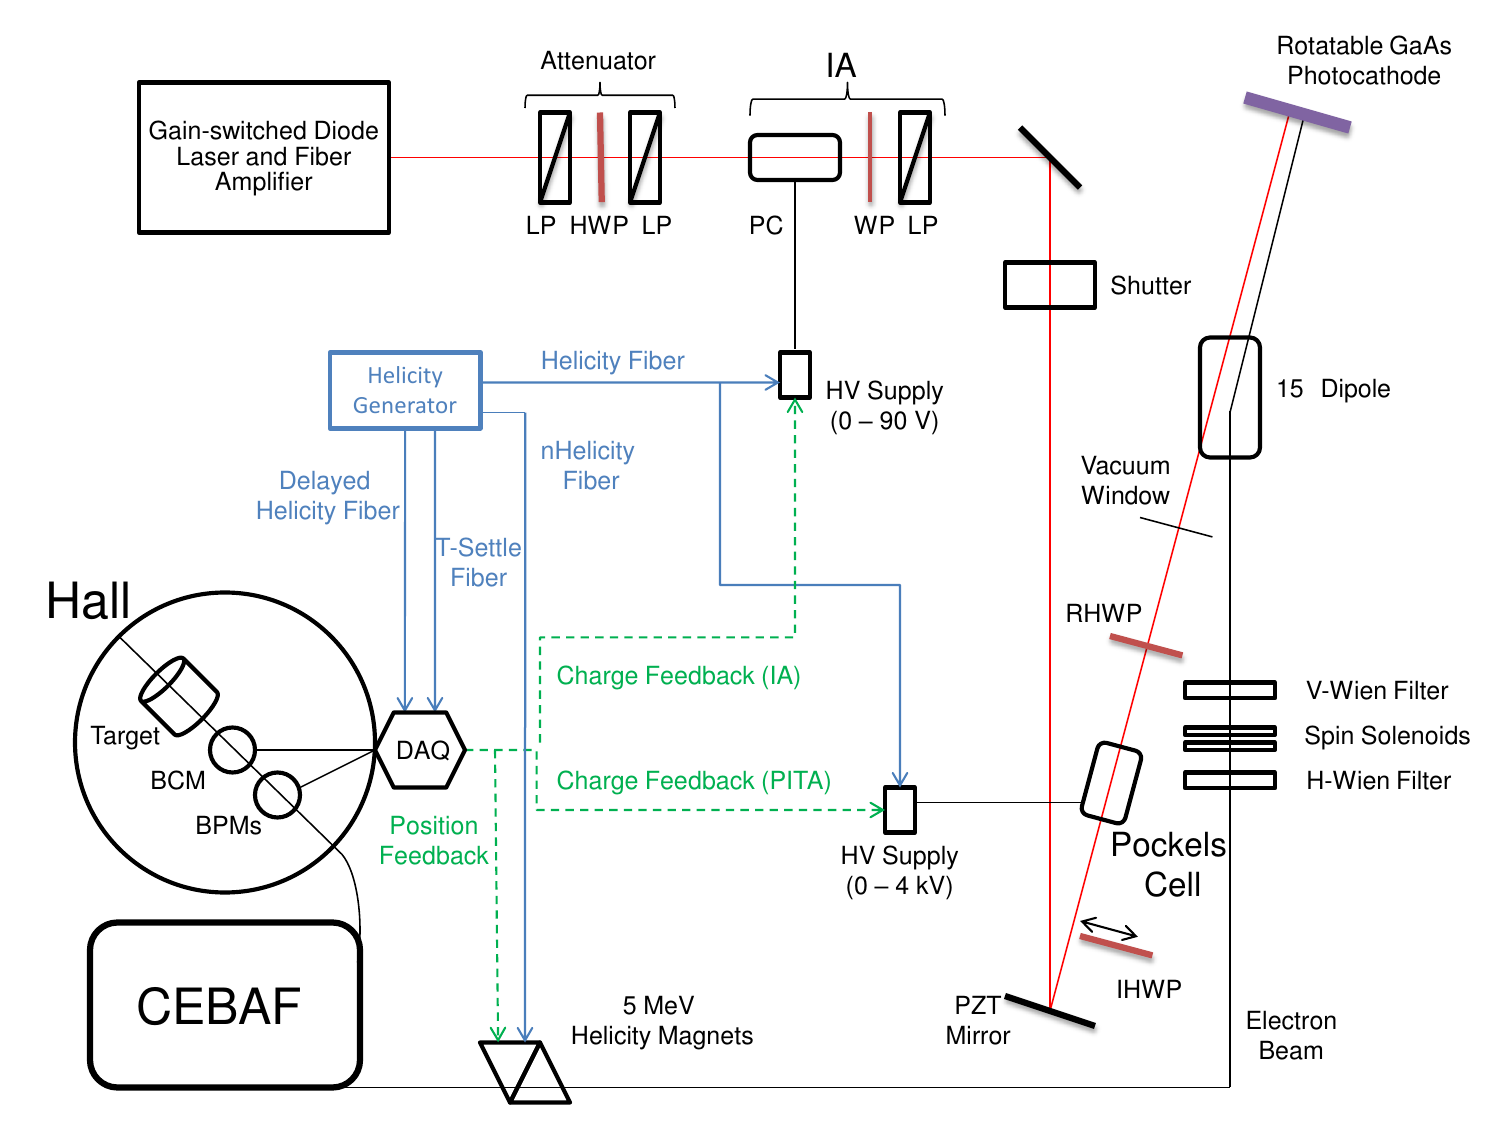
\includegraphics[width=\linewidth]{injector}
    \caption{The laser system at the CEBAF injector}
    \label{fig:injector}
\end{figure}

\begin{figure}[h!]
    \begin{tikzpicture}
	\tikzstyle{explain} = [align=center] 
	\begin{scope}
	    \node[anchor=south west, inner sep=0] (image) at (0, 0)
	    {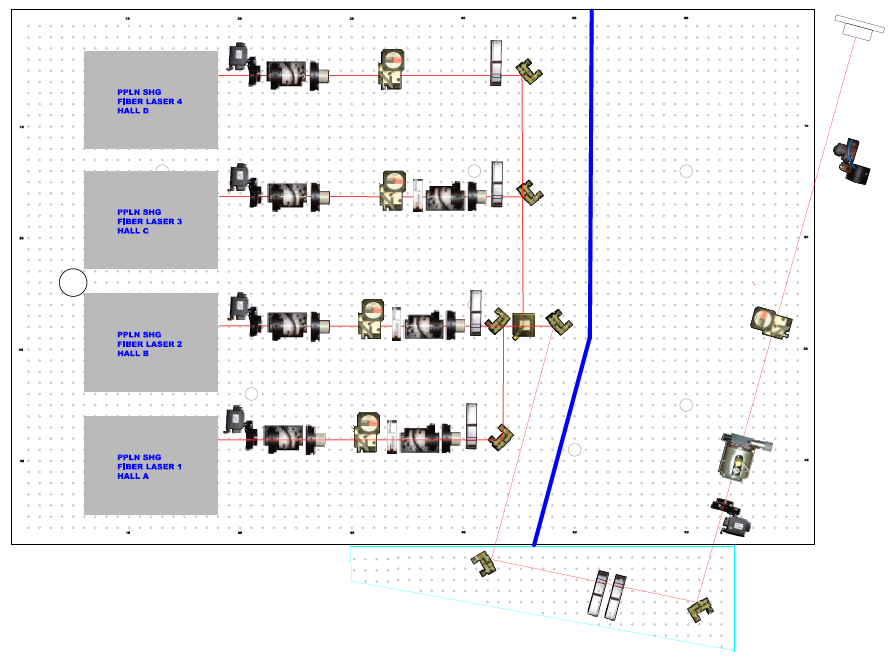
\includegraphics[width=\linewidth]{laser_table}};
	    \begin{scope}[x={(image.south east)},y={(image.north west)}]
		\node [blue,ultra thick] at (0.06,0.3) {\textbf{A}};
		\node [blue,ultra thick] at (0.06,0.49) {\textbf{B}};
		\node [blue,ultra thick] at (0.06,0.67) {\textbf{C}};
		\node [blue,ultra thick] at (0.06,0.85) {\textbf{D}};

		\node [blue,ultra thick] at (0.47,0.39) {\textbf{IA}};
		\node [blue,ultra thick] at (0.47,0.56) {\textbf{IA}};
		\node [blue,ultra thick] at (0.5,0.75) {\textbf{IA}};

		\node [red] at (0.75,0.23) {\textbf{IHWP}};
		\node [explain,red] at (0.76,0.33) {\textbf{Pockels } \\ \textbf{Cell}};
		\node [red] at (0.78,0.52) {\textbf{RHWP}};
		\node [explain,red] at (0.88, 0.96) {\textbf{Beamline} \\ \textbf{vaccum} \\ \textbf{window}};
	    \end{scope}
	\end{scope}
    \end{tikzpicture}
    \caption{Schematic plot of the laser table.}
    \label{fig:laser_table}
\end{figure}

%%%%%%%%%%%%%%%%%%%%%%%%%
\subsubsection{Pockels Cell}
With a proper electron source to produce polarized electron beams, we need more control 
over the beam polarization. We should be able to flip the beam polarization
quickly while keeping the polarization as stable as possible. It is not easy and time
consuming to manipulate electrons directly, while manipulating photons is much 
easier. One just need to reverse the circular polarization of the incident laser pulse,
the electron beam polarization will be flipped. An easy way to do the job is
a half-wave plate, by inserting it into or retracting it from the optical path,
the phase of the laser pulse will be changed by $\pi$, therefore flipping the laser
circular polarization. 

The drawback of the half-wave plate is that the mechanical movement is not fast enough. 
For PVES experiments, the fast flipping of the beam polarization is done by a component 
called Pockels Cell (PC), which is a Rubidium Titanyle Phosphate (RTP) crystal. 
PC operates based on the Pockels effect, 
which is the production of birefringence in the crystal under an electric field, 
the resulted birefringence is proportional to the strength of the
applied electric field. By applying appropriate high voltage ($\sim 1.5$~kV),
% from Caryn's thesis
PC will act as a quarter wave plate (photon amplitude along fast and low axes
$E_x$, $E_y$ will have a phase difference of $\pm \frac{\pi}{2}$ depending on
the polarity of the applied electric field), converting a linearly polarized laser beam
into a circularly polarized one. And reserve the electric field polarity
will reverse the polarization of the laser beam. This transition can be very
fast, up to 1~kHz, with a dead time of about $60\ \mu$s.
% Moller will go up to 2 kHz, with 10 \mu s settle time

\subsubsection{Polarization Induced Transport Asymmetry (PITA, or Phase Induced Transmission Asymmetry) \cite{Caryn2019}}
The above discussion is an ideal case that PC will be an exact quarter wave
plate and other optical components also work flawlessly. In reality, there is always 
some deviations from the perfect circular polarization,
resulting in systematic effects on beam position, spot size and intensity. If the deviation 
is polarization correlated, it will introduce a false asymmetry to our PV asymmetry 
measurement, which is called the PITA effect. The PITA effect is the dominant
piece of the helicity correlated beam asymmetry (HCBA), which is the largest false asymmetry 
in our measurement.

\begin{figure}[!h]
    \centering
    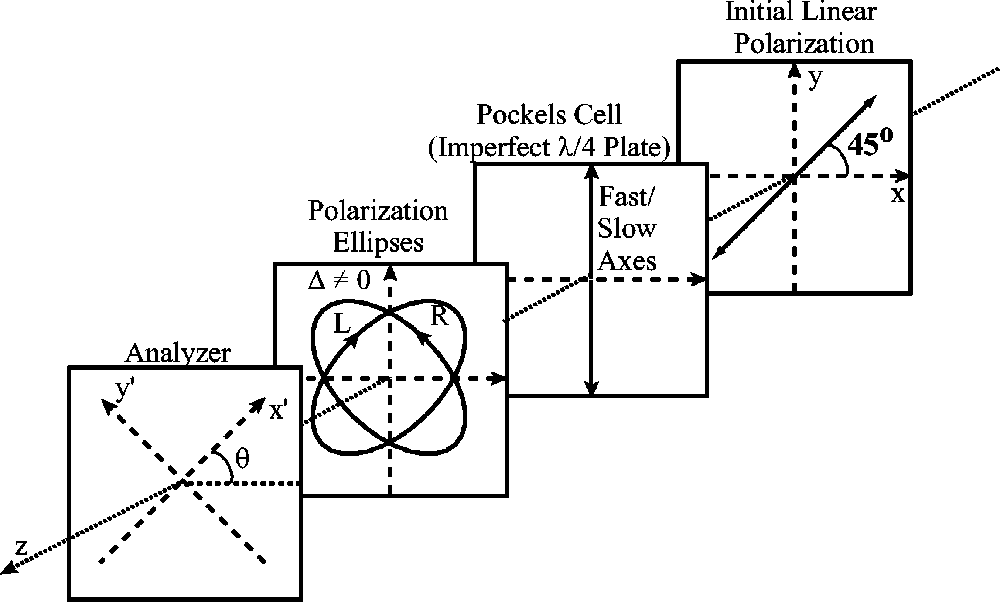
\includegraphics[width=0.5\linewidth]{PC_phase_shift}
    \caption{Phase shift by going through the PC.}
    \label{fig:pc_phase_shift}
\end{figure}

The PITA effect is characterized by the PC induced phase shift $\delta$:
\begin{equation}
    \delta^{R(L)} = \mp\left(\frac{\pi}{2} + \alpha \right) - \Delta
\end{equation}
where $\alpha$ and $\Delta$ represent the symmetric and asymmetric offset phase
shift respectively. The resultant slightly elliptical beam has a residual
linear component, leading to an intensity asymmetry (to first order):
\begin{equation}
    \CA_{I} = \frac{I^R - I^L}{I^R + I^L} = -\frac{\epsilon}{T}[\Delta\cos(2\theta)]
\end{equation}
where $\epsilon/T \ (<<1)$ defines the ``analyzing power'' with $\epsilon = T_{x'} - T_{y'}$ 
and $T = (T_{x'} + T_{y'})/2$.
$T_{x' (y')}$ is the transmission coefficient along the axis x' (y') of the
downstream analyzer. $\theta$ is the angle between the PC's fast axis and the 
$x'$ axis of the analyzer.

Considering other optical components along the laser path, like the rotatable half-wave plate 
(RHWP) and the vacuum window, the unknown tiny birefringence in these components will also 
contribute to $\Delta$, resulting in a modified intensity asymmetry:
\begin{equation}
    \CA_{I} = \frac{I^R - I^L}{I^R + I^L} = -\frac{\epsilon}{T}[\cos(2\theta)\cdot(\Delta - \Delta^0)]	\\
\end{equation}
where $\Delta^0$ represents the asymmetric offset phase shift due to all other components.

To minimize the intensity asymmetry, one would like to keep $\Delta - \Delta^0$
as small as possible. Fortunately, $Delta$ is tunable, by changing the applied
electric field. As shown in Fig.~\ref{fig:injector}, our charge feedback system
will monitor the charge intensity asymmetry and automatically adjust the HV 
supplied to the PC to maintain a small $\CA_I$. Over PREX-II and CREX, the average charge
intensity asymmetry is about 100~ppb.

As shown in Fig.~\ref{fig:injector}, the charge feedback system also
controls the HV supply of the Intensity Attenuator (IA). IA, together with
the slit in the beam chopper, control the intensity of the outgoing electron beams
($\Delta$ does a fine tune to the beam intensity). So, IA also
plays a key role in achieving a small charge intensity asymmetry by equalizing
beam intensities across helicity states.

Another important element is the RHWP, which lies downstream the PC.
It helps to equalize any residual linear polarization left in the PC to establish 
a quantum efficiency (QE) independent of helicity.

\subsubsection{Slow Helicity Reversal}
Fast reversal of the PC can minimize a lot of random noise from beam and target
density fluctuations. Nevertheless, some helicity correlated (HC) false asymmetries
remain, such as the electronic pickup between accelerator electronic systems and 
the experimental DAQ system or the residual birefringence effect. It is the 
job of the slow helicity reversal to cancel these systematic false asymmetries.

There are two methods to make slow helicity reversal -- the insertable half-wave plate (IHWP) 
and the double Wien Filters. Prior to 2009, IHWP was the only available approach
at CEBAF to do slow helicity reversal. A new mechanism was introduced during 
PREX-I and Qweak experiments for better systematic precision -- the wien filter.

The IHWP lies upstream of the PC, as said above, it is easy to change the beam 
helicity by inserting or retracting the IHWP. Slow helicity reversal enables us 
to identify the possible systematic uncertainties. The idea is simple, 
assume the true and a systematic false asymmetry to be $\CA_0$ and $\Delta \CA$,
then the measured asymmetry by inserting (retracting) the IHWP will be:
\begin{equation}
    \CA^{+(-)} = \pm \CA_0  + \Delta \CA
\end{equation}
Because IHWP doesn't affect the systematic uncertainty, the true asymmetry will be:
\begin{equation}
    \CA_0 = \frac{\CA^+ - \CA^-}{2}
\end{equation}

As good as the IHWP, it resolves only some of the HC beam variations, namely
the residual birefringence from the laser optical system and is powerless in dealing
with other HC effects, like HC beam size variations that are introduced via
PC focusing \cite{osti_1059486}, which is addressed by the wien filter.

The double wien filters manipulate the electron spin directly by EM fields 
without affecting the electron movement and is able to achieve any spin orientation.
It consists of two wien filters and two intervening solenoids between them, as
shown in Fig~\ref{fig:double_wien_filters}.
A wien filter is such a cavity with proper electric and magnetic fields ($qE = qvB$)
that are perpendicular to each other and to the electron moving direction, so that it 
rotates only the electron spin.

Electrons coming from the photocathode are longitudinally polarized,
the vertical wien filter will make the electron spin vertical oriented, then the
spin will be rotated to left/right by the following spin solenoid, depending on
the polarity of the solenoid. A wien flip means to change the polarity of the spin solenoid.
Finally, the horizontal wien filter will fine tune the spin direction to optimize 
the longitudinal polarization in the experimental hall. 

Note that electrons at the exit of the double wien filters are not longitudinally polarized, 
because electron spin will precess when travel through the accelerator, causing a rotation 
in the horizontal plane. Therefore, a carefully selected initial spin direction is 
needed to make sure the spin is (anti) parallel to the electron momentum at the target.
This tells another function of the double wien filters: to set a non-longitudinal 
initial spin to cancel out the shift caused by the spin precession during acceleration, 
so that the electron beam is exactly longitudinally polarized at the target.
\begin{figure}[!h]
    \centering
    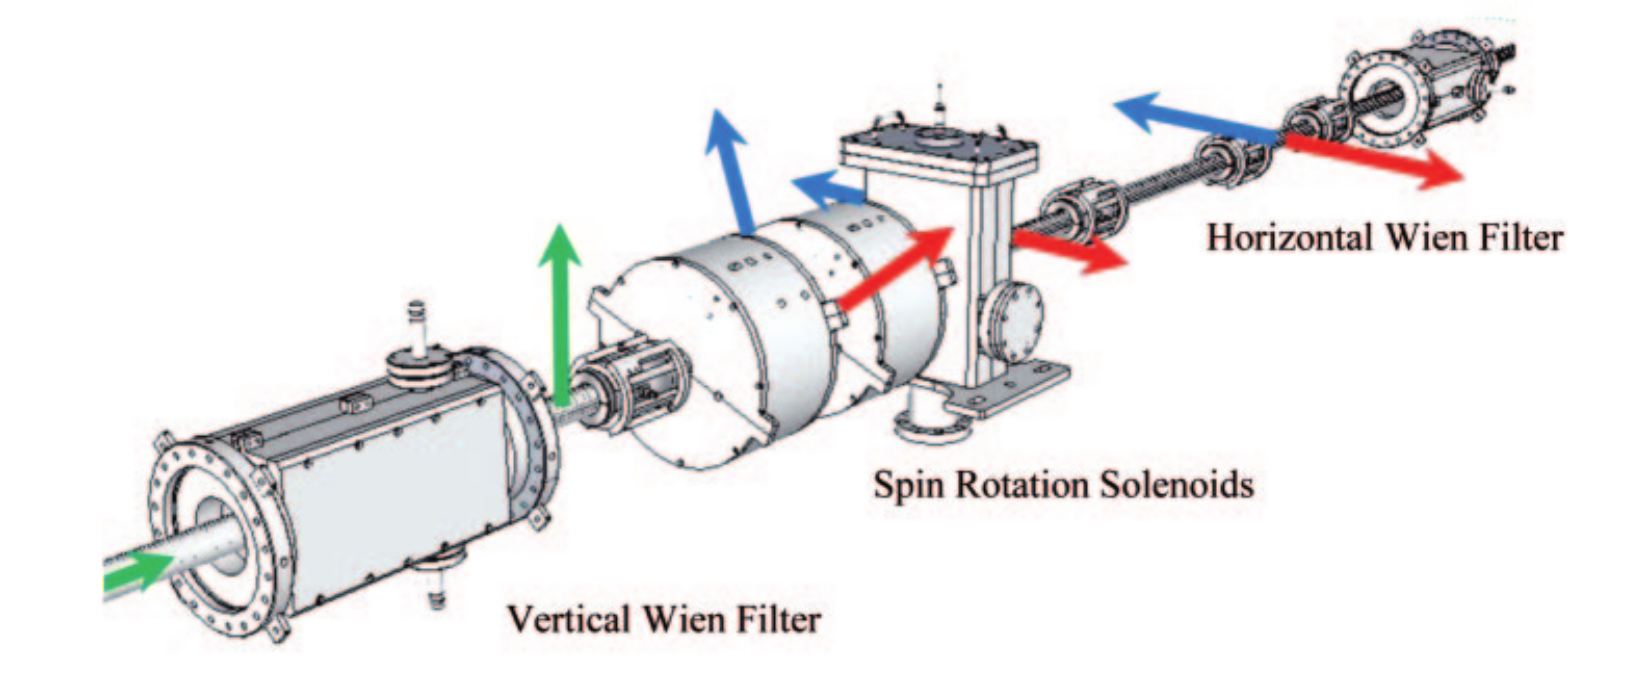
\includegraphics[width=0.5\linewidth]{wien_filter}
    \caption{Schematic plot of the double wien filters. Electron beam travels from left
    to right. \cite{osti_1059486}}
    \label{fig:double_wien_filters}
\end{figure}

With both the IHWP and the double wien filters, we are able to cancel most 
systematic false asymmetries, achieving very small systematic errors.
\begin{comment}
    IHWP
    % https://www.jlab.org/accel/inj_group/docs/2009/parity_Ops_Training_05Aug09.pdf
    \begin{itemize}
	\item Cancels electronic cross talk and Pockels Cell steering
	\item  Residual linear polarization effects do not cancel
	\item Spot size asymmetry, which we cannot measure, does not cancel
    \end{itemize}

    Wine filters and solenoid
    \begin{itemize}
	\item Cancels all helicity-correlated beam asymmetries from Injector including spot size
    \end{itemize}
\end{comment}

%%%%%%%%%%%%%%%%%%%%%%%%%%%%%%%%%%%%%%%%%%%%%%%%
\subsection{Polarimeters}
With polarized electron beams, we need to measure their polarizations.
There are three polarimeters to measure the beam polarization: the Mott polarimeter
at the injector and the Compton and Moller polarimeters in Hall A. As their names
imply, they use the cross section asymmetry of the Mott, Compton and Moller
scatterings to measure the polarization of the electron beam. Since these are
all pure quantum electrodynamics (QED) processes, their cross sections are 
well understood and analyzing powers are easily calculable to high orders.

While the Mott and Moller measurements are invasive, they can't be done frequently
(Moller measurement happens about every 10 days).
The non-invasive Compton polarimeter is the only choice for beam polarization monitoring. 
The Mott polarimeter measures the beam polarization before it enters the accelerator, 
so it is not used for the determination of the beam polarization during PREX-II/CREX.

%%%%%%%%%%%%%%%%%%%%%%%%
\subsubsection{Mott Polarimeter}
\begin{figure}[!h]
    \centering
    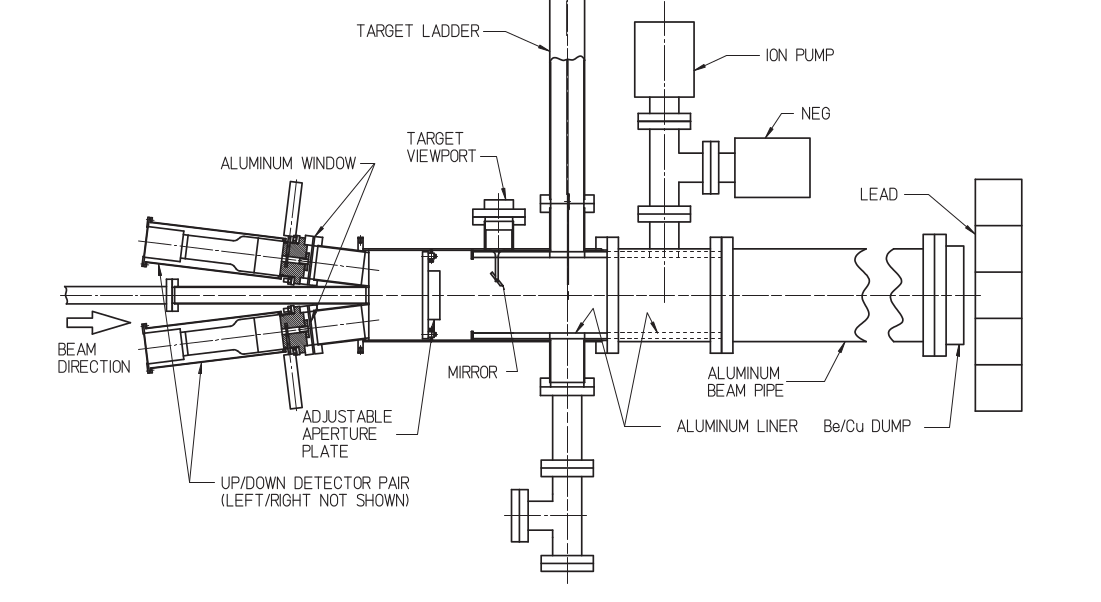
\includegraphics[width=0.5\linewidth]{Mott_polarimeter}
    \caption{Schematic plot of the Mott polarimeter. It has 4 symmetric detector
    ports (up and down, left and right -- left/right detectors are not shown in the plot). 
    The back scattering angle is $172.6^\circ$, where the highest analyzing power 
    is achieved from theoretical calculations of the Sherman function.
    \cite{PhysRevC.102.015501}}
\end{figure}
The 5-MeV Mott polarimeter lies at the CEBAF injector, between the double wien filters
and the Injection Chicane, it measures the single spin cross section asymmetry
of 5~MeV electron beams scattered off a high-Z target. Comparing the measurement
to the Sherman function $S$ \cite{PhysRev.103.1601} -- the analyzing power, one will 
derive the transverse polarization of the beam:
\begin{equation}
    \CA_{LR} = \frac{N_L - N_R}{N_L + N_R} = S(\theta)\vec{\CP}\cdot \hat{\vec{n}}
\end{equation}
where $\theta$ is the scattering angle and $\hat{\vec{n}}$ is the unit normal 
vector of the scattering plane. The same formula applies to the up-down asymmetry.
\begin{figure}
    \centering
    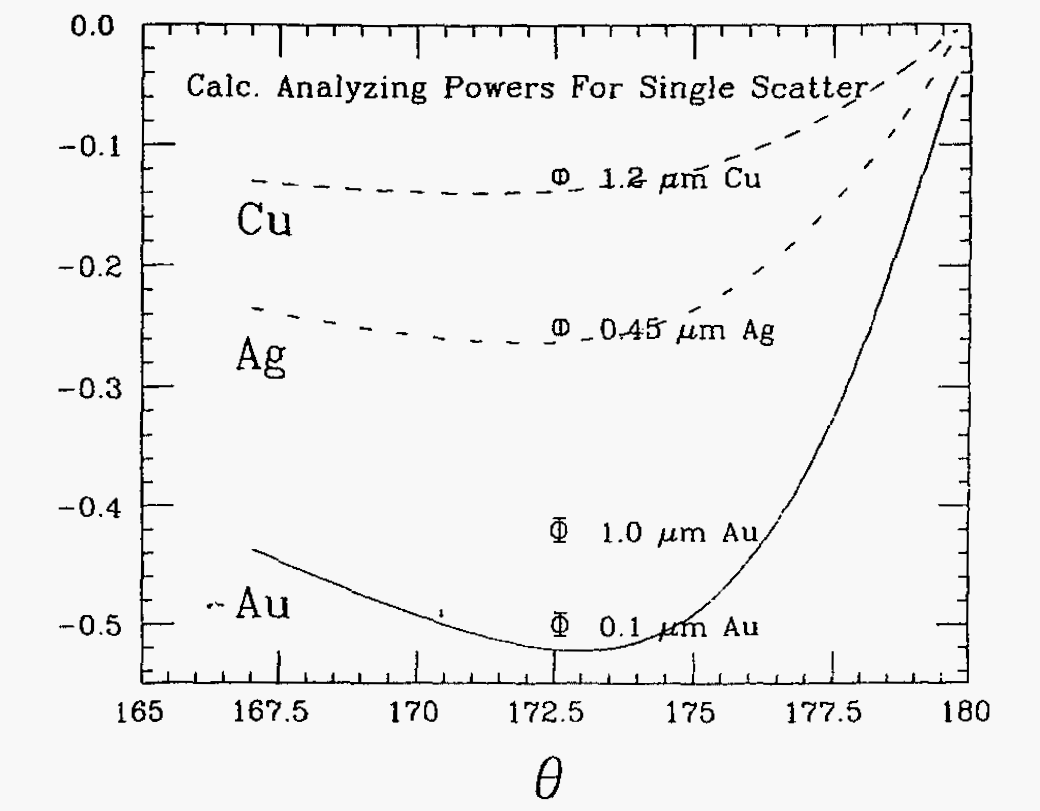
\includegraphics[width=0.5\linewidth]{Mott_asym_1}
    \caption{The Sherman function for different high-Z targets at 5~MeV, dots
    represent experimental measurements.}   % FIXME reference
\end{figure}
Because the asymmetry comes from the coupling of the electron spin and the induced
magnetic field by the nucleus in the electron's rest frame (spin-orbit coupling), 
the scattering potential is:
\begin{equation}
    V(r, \vec{L}, \vec{S}) = V_{\text{Coulomb}} + V_{\text{so}} (r, \vec{L}, \vec{S}) 
    = \frac{Ze}{r} + \frac{Ze^2}{2m^2r^3}\vec{L}\cdot \vec{S}
\end{equation}
So only the transverse polarization, rather than the longitudinal one, can be 
measured using a Mott polarimeter. Nevertheless, it provides an
independent check of the initial beam polarization from the injector and its high
precision (its total uncertainty can be as small as 0.61\% \cite{PhysRevC.102.015501}) 
helps to normalize the polarization measurement in the experimental halls.

%%%%%%%%%%%%%%%%%%%%%%%%
\subsubsection{Compton Polarimeter}
% Compton photon detector: https://prex.jlab.org/DocDB/0002/000273/002/Cornejo_and_Quinn_ComptonPhoton_CREX_PREX_Nov_2018.pdf
The Compton polarimeter locates at the entrance to Hall A (about 20~m upstream the 
target chamber), using the elastic scattering between polarized photons and electrons
to measured the polarization of the electron beam. As shown in Fig.~\ref{fig:compton_pol},
when the Compton polarimeter is on, the electron beam will be bent into the 
Compton Chicane to interact with the polarized photons nearly head-on (with a tiny
crossing angle of 23.5~mrad). The Fabry-Perot Cavity
is locked to and filled with circularly polarized ($> 99\%$) green laser beam
($\lambda = 532$~nm, $E = 2.334$~eV).
The back-scattered photons will be detected by a Gadolinium Orthosilicate (GSO) 
% GSO (low energy) or $\text{PbWO}_4$ 
crystal calorimeter right of the interaction region, while the
unscattered electron beam will be sent back to the beam pipe to bombard the target. 
Due to interaction with photons, the scattered electrons will be less energetic than
the incoming ones. Under the same dipole field, the scattered electrons will
be bent more than the unscattered ones, as shown by the red dash line 
in Fig.~\ref{fig:compton_pol}. This 
separation allows to count the scattered electrons, together with the measurement
of scattered photons, one can identify the scattering asymmetry and then the polarization
of the electron beam.
\begin{figure}[h!]
    \begin{subfigure}[c]{0.55\linewidth}
	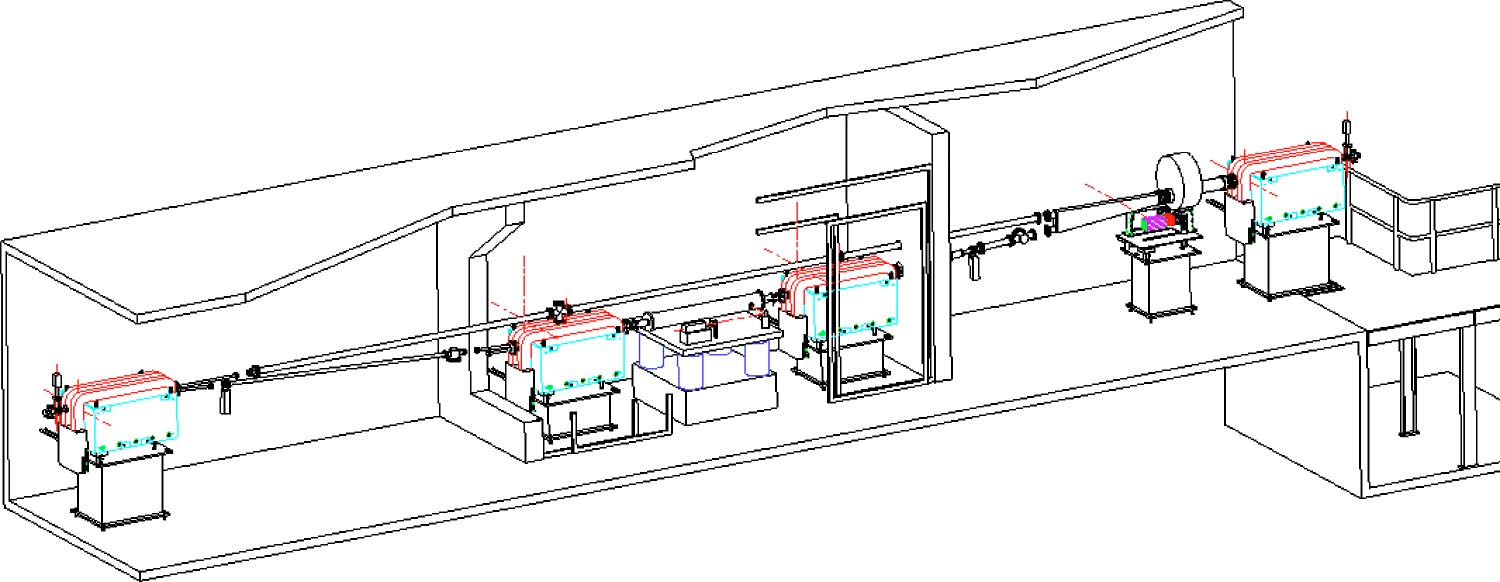
\includegraphics[width=\linewidth]{Compton_setup}
    \end{subfigure}
    \begin{subfigure}[c]{0.55\linewidth}
	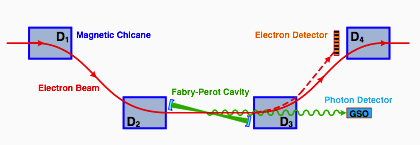
\includegraphics[width=\linewidth]{Compton_beam_path}
    \end{subfigure}
    \caption{Left: schematic plot of the Compton Chicane \cite{PhysRevSTAB.7.042802}; 
    Right: schematic plot of the electron-photon scattering.} 
    \label{fig:compton_pol}
\end{figure}

The energy of the scattered photon is:
\begin{equation}
    E_\gamma \approx E_{\text{laser}} \frac{4a\gamma^2}{1 + a\theta^2_\gamma \gamma^2}
\end{equation}
where $\gamma = E_{\text{beam}}/m_e$ is the Lorentz factor of the incoming electron, 
$a = \frac{1}{1 + 4\gamma E_{\text{laser}}/m_e}$ and $\theta_\gamma$ is the scattering
angle w.r.t. the electron momentum. The maximum energy of the scattered
photon appears at $\theta_\gamma = 0$, which is the back scattering. 
For PREX-II (CREX) beam energy of 0.95 (2.2)~GeV, $E_\gamma^{\text{max}} \sim$ 32.55 (167.02)~MeV.

Define $\rho = \frac{E_\gamma}{E_\gamma^{\text{max}}}$, the cross section for the unpolarized
Compton scattering will be:
\begin{equation}
    \frac{d\sigma}{d\rho} = 2\pi r_0^2 a 
    \left[ \frac{\rho^2 (1-a)^2}{1 - \rho(1-a)} + 1 + \left( \frac{1 - \rho(1+a)}{1- \rho(1-a)}\right)^2\right]
\end{equation}
$r_0 = \frac{\alpha \hbar c}{mc^2}$ is the classical electron radius; then the
analyzing power is:
\begin{equation}
    \CA_l = \frac{\sigma^\rightarrow_\Rightarrow - \sigma^\leftarrow_\Rightarrow}
    {\sigma^\rightarrow_\Rightarrow + \sigma^\leftarrow_\Rightarrow}
    = \frac{2\pi r_0^2 a}{d\sigma/d\rho}(1 - \rho(1+a))\left[ 1 - \frac{1}{(1 - \rho(1-a))^2}\right]
\end{equation}
\begin{figure}
    \centering
    \includegraphics[width=0.5\linewidth]{compton_asym}
    \caption{The Compton analyzing power increases with the incoming electron energy. 
    Note that the analyzing power will change sign at $\rho \sim 0.5$ for both PREX-II
    and CREX beam energies.}
\end{figure}

The measured asymmetry will be:
\begin{equation}
    \CA_{\text{exp}} = \CP_{e}\CP_{\gamma}\CA_{l} = \frac{N_{\gamma}^R - N_{\gamma}^L}{N_{\gamma}^R + N_{\gamma}^L}
    \Rightarrow
    \CP_e = \frac{\CA_{\text{exp}}}{\CP_{\gamma}\CA_{l}}
\end{equation}
The advantage of the Compoton polarimeter is that it can tolerate quite high current
(up to $\sim 200 \ \mu$A at JLab), plus its non-invasive operation, making it a beam 
polarization monitor. The disadvantage is, compared to the Mott or Moller polarimeter,
its analyzing power is quite low at GeV energy level, while increase the beam
energy will lead to a high background in the photon detection due to synchrotron 
radiation. Overall, the Compton polarimeter is able to achieve a 1\% absolute systematic
uncertainty.

%%%%%%%%%%%%%%%%%%%%%%%%
\subsubsection{Moller Polarimeter}
% low current only
The Moller polarimeter lies downstream of the Compton polarimeter and upstream 
of the target chamber. It uses elastic electron-electron scattering to measure the
cross section asymmetry between beams with different polarizations. 
\begin{equation}
    \begin{gathered}
	\frac{d\sigma}{d\Omega} = \frac{d\sigma_0}{d\Omega} (1 + \sum_{i,j=x,y,z} \CP_b^i \cdot \CP_t^j \cdot \CA_{ij}(\theta_{CM})) \\
	\frac{d\sigma_0}{d\Omega} = \frac{\alpha^2}{s} \left( \frac{4 - \sin^2\theta_{\mathrm{CM}}}{\sin^2\theta_{\mathrm{CM}}}\right)^2 
    \end{gathered}
    \label{eq:moller_xsection}
\end{equation}
With $\frac{d\sigma_0}{d\Omega}$ being the unpolarized Moller scattering cross section,
$s$ the Mandalstam variable: $s = 2m_e(E+m_e) \approx 2m_e^2\gamma$,
$\CP_b \ (\CP_t)$ the polarization of the beam (target),
$\theta_{\mathrm{CM}}$ and $\CA_{ij}$ the scattering angle and analyzing power in the COM frame. 

Assuming incoming electrons move in the z direction and the scattering happens
in the xz plane, then in the ultra-relativistic limit:
\begin{equation}
    \begin{gathered}
	\CA_{zz} = \frac{\sin^2\theta_{CM} (7 + \cos^2\theta_{\mathrm{CM}})}{(3+\cos^2\theta_{\mathrm{CM}})^2},
	\quad
	\CA_{xx} = -\CA_{yy} = \frac{\sin^4\theta_{\mathrm{CM}}}{(3+\cos^2\theta_{\mathrm{CM}})^2}	\\
	\CA_{xz} = \CA_{zx} = \frac{2\sin^4\theta_{\mathrm{CM}}\cos\theta_{\mathrm{CM}}}{\gamma(3+\cos^2\theta_{\mathrm{CM}})^2},
	\quad
	\CA_{xy} = \CA_{yz} = \CA_{yz} = \CA_{zy} = 0
    \end{gathered}
\end{equation}
$\CA_{zz}$ is maximized to be $\frac{7}{9}$ at $\theta_{\mathrm{CM}} = 90^\circ$.
This $\theta_{\text{CM}}$ value was used in the Moller measurement.

The polarized target electrons come from a magnetized Fe-alloy foil, which is 
saturated by a very strong (4~T) longitudinal magnetic field created by 
superconducting Helmholtz coils, as shown in Fig.~\ref{fig:moller_polarimeter}. 
So Eq.~\ref{eq:moller_xsection} is simplified to:
\begin{equation}
    \frac{d\sigma}{d\Omega} = \frac{d\sigma_0}{d\Omega} ( 1 + \CP_b^z \cdot \CP_t^z \cdot \CA_{zz}(\theta_{CM}))
    \label{eq:moller_xsection_1}
\end{equation}
The Moller pair (the scattered incident electron and recoil target electron)
centered around $\theta_{\text{CM}} = 90^\circ$ ($\theta_{\text{lab}} < 3^\circ$), 
are separated from the undeflected beam by set of magnets, then goes through
collimators (at the exit of the dipole, not shown in Fig.~\ref{fig:moller_polarimeter}) 
that define the acceptance, and finally is detected by electron detectors in coincidence.
The measured asymmetry between spin-parallel and anti-parallel cross section is:
\begin{equation}
    \CA_{\text{exp}} = \frac{N^+ - N^-}{N^+ + N^-} = \CP_b \CP_t \langle \CA_{zz} \rangle 
    \Rightarrow
    \CP_b = \frac{\CA_{\text{exp}}}{\CP_t \langle \CA_{zz} \rangle}
\end{equation}
with $\langle \CA_{zz} \rangle$ being the average analyzing power over the acceptance,
which is about 0.75 for PREX-II and CREX.

% https://prex.jlab.org/DocDB/0005/000502/002/CREX_Moller_Polarimetry_Systematics_Oct_2021.pdf
The target foil is cooled by conduction through the target, whose temperature 
will climb quickly with increase beam current, causing damage to the target
polarization. Therefore the Moller polarimeter can only operate at very low current ($\lesssim 1\mu$A).
The extrapolation from the polarization measurement at a low current to a high current
where PREX-II and CREX run at, is a large source of systematic uncertainty.
During PREX-II and CREX, the target polarization was measured to be $\CP_t \sim 8\%$,
leading to an effective analyzing power of $\CA_{\text{eff}} = \CP_t\langle \CA_{zz} \rangle \approx 6\%$.
This relative large analyzing power makes the Moller measurement quite precise.
Overall, the Moller polarimeter in Hall A can achieve a systematic uncertainty less
than 1\%.

\begin{figure}[!h]
    \centering
    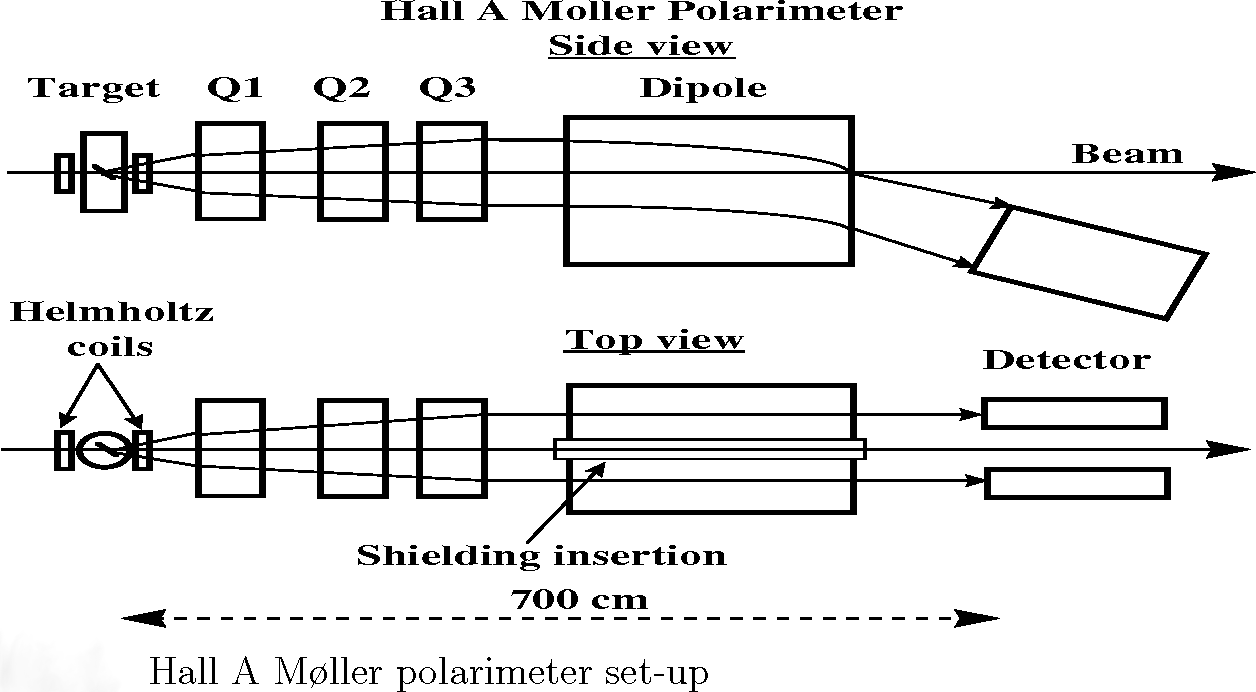
\includegraphics[width=0.7\linewidth]{moller_setup}
    \caption{Schematic plot of the Moller Polarimeter.}
    \label{fig:moller_polarimeter}
\end{figure}

%%%%%%%%%%%%%%%%%%%%%%%%%%%%%%%%%%%%%%%%%%%%%%%%%%%%%%%%%%%%%%%%%%%%%%%%
\section{Monitors}
Besides beam polarization, another significant source of systematic uncertainty
is the beam false asymmetry -- the difference in beam position, angle, energy and
current between different helicity states. Because there is no way to ensure
exactly the same beam parameters between different helicity states, even with the fast
helicity flipping. We monitor these quantities with redundant specialised devices
-- beam position monitors and beam current monitors. For PREX-II
and CREX, there is another independent monitor system -- small angle monitors (SAMs).
There monitors are able to measure the beam difference as precise as:
$$ \Delta x \sim 10\ \mathrm{nm} \quad \Delta x' \sim 1\ \mathrm{nrad} \quad \Delta p/p \sim 0.0001 \quad \Delta I/I \sim 100 \ \mathrm{ppb} $$
\begin{figure}[!h]
    \centering
    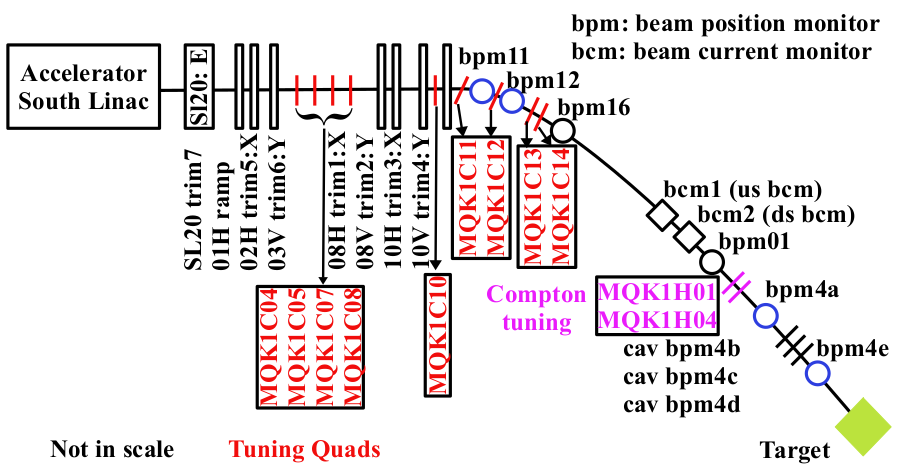
\includegraphics[width=0.5\linewidth]{beam_monitor_and_modulation}
    \caption{Schematic plot of the Hall A beam monitor system and beam modulation system}
    \label{fig:hall_a_monitors_and_modulation}
\end{figure}

\begin{comment}
    \begin{itemize}
	\item beam correlations
	\item monitor precision (resolution): double difference width
	\item noise
	\item pedestal: calibration
	\item cross-correlation
    \end{itemize}
\end{comment}

%%%%%%%%%%%%%%%%%%%%%%%%%%%%%%%%%%%%%%%%%%%%%%%%
\subsection{BPMs}
% Cross check, and unfold beam fluctuation noise from instrumentation noise
Hall A has a series of BPMs along the beam pipe leading to the target chamber
to monitor the beam conditions, among them, six switched electrode electronics (SEE) 
stripline BPMs are important to PREX-II and CREX, their readouts are used to 
extract beam parameters. They are shown in Fig.~\ref{fig:hall_a_monitors_and_modulation}. 
BPM4A and BPM4E locate 5.725~m and 1.642~m upstream of the target chamber, 
they are used to determine the beam position and angle at the target. BPM11 and BPM12
are positioned on the arc area to measure the beam energy using the bending 
radius of the electron trajectory. BPM1 and BPM16 are backup monitors.

A stripline BPM consists of a 4-wire antenna array of open ended thin wire striplines, 
the voltage induced by the electron bunch in each electrode is sensitive to the beam position.
Therefore one can extract (x', y') positions from opposite 2 pickup signals.
\begin{figure}[!h]
    \centering
    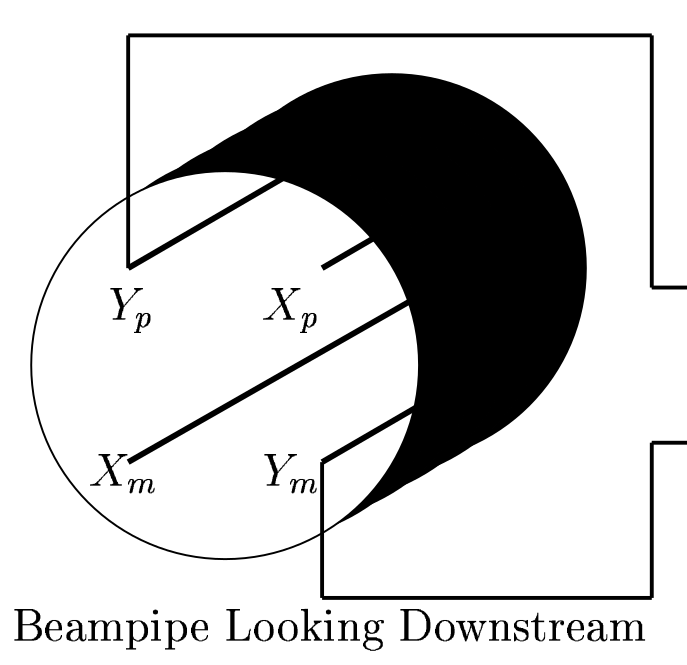
\includegraphics[width=0.35\linewidth]{stripline_bpm}
    \caption{Schematic plot of a stripline BPM.}
\end{figure}
\begin{equation}
    x' = \frac{1}{S_x} \frac{X_p - X_m}{X_p + X_m}   \qquad
    y' = \frac{1}{S_y} \frac{Y_p - Y_m}{Y_p + Y_m}   
\end{equation}
where the proportional constant $S_x$ ($S_y$) is the position sensitivity. 
The pickup voltage responds linearly to the beam displacement when it
is small. In the case of Hall A BPMs, the four striplines are rotated $45^\circ$
w.r.t. to the hall coordinate system, so a $-45^\circ$ rotation is needed to recover
the hall (x, y) from the extracted BPM (x', y').

Besides these stripline BPMs, PREX-II and CREX also utilized 3 cavity BPMs (see discussion below),
shown as bpm4b/c/d between BPM4a and BPM4e in Fig.~\ref{fig:hall_a_monitors_and_modulation},
to measure beam conditions for low current calibration runs. Because stripline
BPMs don't work when beam current is lower than $0.5\ \mu$A. These cavity
BPMs are not used in normal production runs.

%%%%%%%%%%%%%%%%%%%%%%%%%%%%%%%%%%%%%%%%%%%%%%%%
\subsection{BCMs}
One technique to measure the beam current is current transformation.
Various BCMs based on this idea may have different designs, features and performances, 
the key component is the same -- the current transformer (CT). When beam bunch 
travel through the beam pipe, it will induce a magnetic field in the beam pipe (the core), 
which in turn will induce a current in the secondary winding (toroid), 
whose output is proportional to the beam current. 
To make a precise measurement, it is important to shield any outside magnetic 
field and separate the segment of beam pipe where the BCM lies in from the rest.

The BCM system in Hall A consists of two radio frequency (rf) cavities and
an unser monitor in between, as shown in Fig.~\ref{fig:BCMs}. 
The unser monitor is a parametric current transformer (PCT),
which will output a direct current (DC) voltage equivalent to 4~mV per $\mu$A of beam \cite{987367}.
% With good magnet shielding, the unser monitor is able to measure the beam current
% at a precision of ???.

In PREX-II and CREX, the unser monitor is not used for the beam current measurement,
because its voltage output drifted quickly after only a few minutes of running.
Instead, it is used to calibrate the rf-cavity monitors on either side of it,
whose readout is used for the runtime beam current measurement.
\begin{figure}[!h]
    \centering
    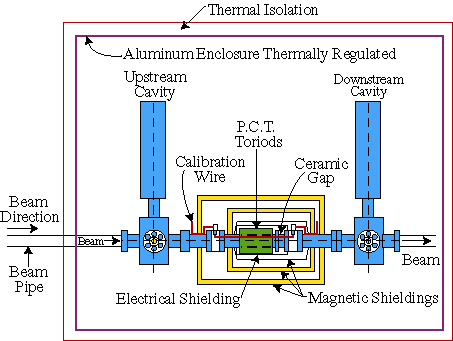
\includegraphics[width=0.5\linewidth]{bcm}
    \caption{Hall A BCM system \cite{987367}.}
    \label{fig:BCMs}
\end{figure}

A rf cavity is a metallic chamber that sustains an EM field 
(infinite number of resonant EM modes), by special design of its shape, a particular
EM mode can efficiently transfer energy to or from a charged particle. The 
frequently heard accelerating cavity need to provide an electric field along
beam velocity; while a decelerating cavity, which will absorb energy
from the coming charged particles, can be used as a beam diagnostic monitor.
The induced voltage is proportional to the traversing charge q:
\begin{equation}
    V = 2k_{loss} q
\end{equation}
where $k_{loss}$ is the loss factor, which depends only on the electric field
distribution, therefore is sensitive to the beam position and particle velocity.
To measure beam intensity, one would prefer the EM mode whose electric field
doesn't depend on r position, these are $\text{TM}_{\text{010}}$ like modes;
while for measurement of beam position, exactly the opposite is wanted, the
electric field should have an azimuth angle and r dependence, which are $\text{TM}_{\text{110}}$
like modes.
\begin{figure}[!h]
    \centering
    \begin{subfigure}[c]{0.5\textwidth}
	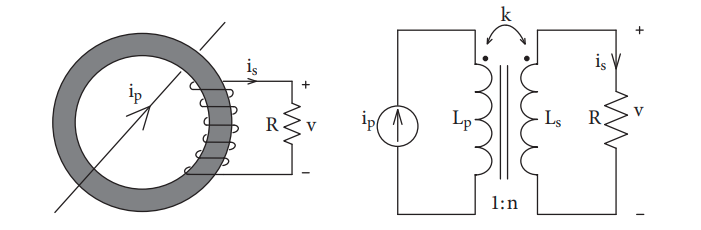
\includegraphics[width=\linewidth]{current_transformer}
    \end{subfigure}
    \begin{subfigure}[c]{0.55\textwidth}
	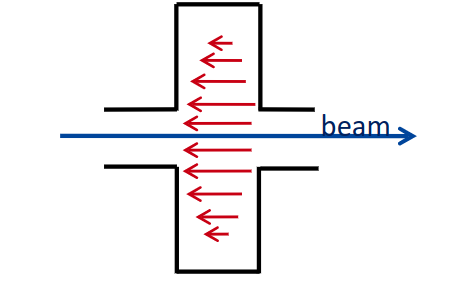
\includegraphics[width=0.52\linewidth]{TM010}
	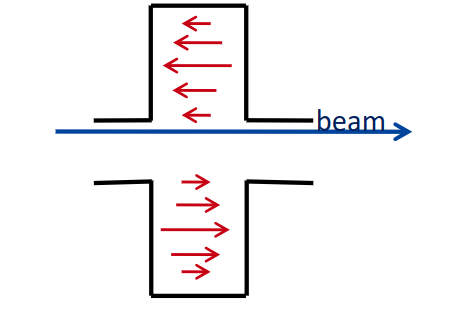
\includegraphics[width=0.46\linewidth]{TM110}
    \end{subfigure}
    \caption{Up: Schematic plot of the current converter; 
    Down: $\text{TM}_{010}$ and $\text{TM}_{110}$ modes, the red arrows indicate the electric field.}
\end{figure}

The 2 rf-cavity current monitors are of Pill box type (the electric field is
concentrated near axis, while the magnetic field is concentrated at outer
cylindrical wall), which operates at $\text{TM}_\text{010}$ mode. The voltage 
readout will be down-converted to lower frequencies signals, then filtered, 
amplified and further processed before writing into the data stream. Due to
the non-linearity of the readout converter at low currents ($\lesssim 5\ \mu$A), 
actually 3 signals (the same signal with different gains: x1, x3 and x10) are
recorded to extend the linear region to low currents, at the expanse of saturation
at high currents \cite{halla_manual}.
% readout converter linear region: ~5 - > 200 uA

%%%%%%%%%%%%%%%%%%%%%%%%%%%%%%%%%%%%%%%%%%%%%%%%
\subsection{SAMs}
For further understanding of beam dynamics, electronic noise and the possible target 
boiling effect, a luminosity monitoring system, called the small angle monitors, 
was installed in the dump pipe, about 7~m downstream of the target pivot. As shown
in Fig.~\ref{fig:sams}, the SAMs system consist of 8 detector modules, symmetrically 
positioned around the dump pipe. Each detector module has a quartz tile (active 
detector), attached to a lightguide. the Cherenkov light radiated by electrons
will be read out by a PMT at the end of the lightguide. 
As its name implies, SAMs are designed to monitor small angle ($\sim 1^\circ$)
scattered and secondary flux from the target, thus it can also be used to
inspect the target conditions. E.g., a bubble in the target that forms and disappears
within one helicity window is unknown to both BPMs and BCMs, but SAMs will see it.
Each detector's readout is sensitive to beam parameters.
E.g., the sum of the readout of a symmetric pair monitors is sensitive to change 
in the beam current and energy, while their difference tells the fluctuation in 
the beam position and angle.
The symmetric design helps to disentangle these beam parameters. So it provide
an independent check of the measurement of BPMs and BCMs and can be used to eliminate
the possible beam or electronic noise.
\begin{figure}[!h]
    \centering
    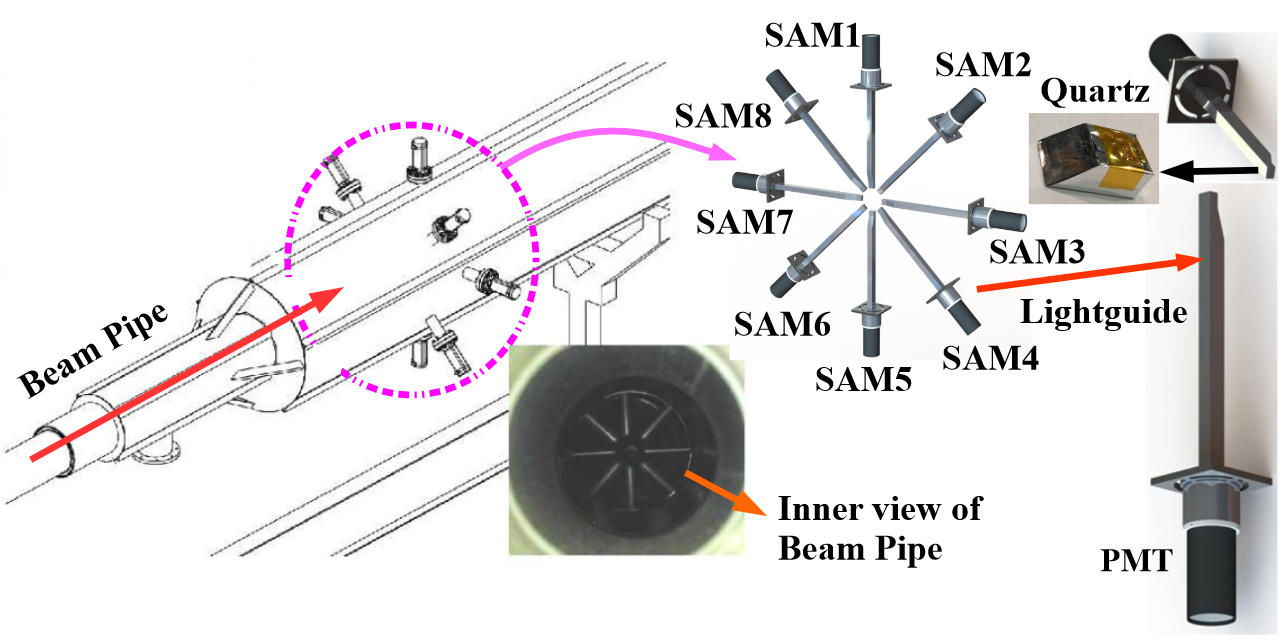
\includegraphics[width=0.8\linewidth]{sams_system}
    \caption{Layout of SAMs \cite{Devi2021}.}
    \label{fig:sams}
\end{figure}

%%%%%%%%%%%%%%%%%%%%%%%%%%%%%%%%%%%%%%%%%%%%%%%%
\subsection{Beam Modulation}
\begin{comment}
It is very important for PVES to control the systematic uncertainty, especially
the one from beam fluctuation (HCBA). Ideally, the electrons bunches with opposite
polarization should have exactly the same intensity and energy, hitting the target 
at the same place with the same angle, which is obviously impossible in reality. 
So we need to correct the false asymmetry introduce by the beam fluctuation. There are a
few methods to do the correction, one of them is the so called Beam modulation.
The idea is to introduce man-made fluctuations to the beam through the 
modulation system, then we can measure the changes in monitors and detectors 
to find the sensitivities of detectors to changes in energy, position and angle,
which will be used to correct the measured asymmetry.
\end{comment}

Another system shown in Fig.~\ref{fig:hall_a_monitors_and_modulation} is the
beam modulation system, which lies in beamline arc right after the Beam Switch Yard 
where electron chains are separated into Hall A/B/C beams.
It consists of 6 air-core coils and an energy vernier in the last cavity of the south LINAC.
The total number of 7 coils provides a redundancy w.r.t. the number of free degrees 
of the beam phase space, making sure to cover the whole beam phase space at the target.  
Coil (trim) 1, 3, 5 are responsible for modulating beam x position and coil 
2, 4, 5 will modulate beam y position.
These coils (vernier) are driven by a VME-DAC (Digital-Analog Converter), 
which in turn is controlled by the parity data acquisition (DAQ).
It takes 4.267~s for each coil (vernier) to modulate the beam, a whole 
modulation cycle takes 85.68~s ($\sim 1$ beam modulation every 10~mins during
run time). 

The beam modulation system is used for beam false asymmetry correction. 
When beam is modulated, BPMs and detectors will record corresponding
changes in their readout. With these values, the detector sensitivity w.r.t. jitters 
in beam parameters can be calculated, which then will be used to correct the
measured asymmetry. Therefore, the modulation should be much larger than the natural
jitters in the beam, a typical position modulation is a sinusoid of amplitude about $200\ \mu$m 
% https://www.arxiv-vanity.com/papers/1208.6513/
and the energy vernier will result in a beam displacement of 0.75~mm in BPM11/12.
% \begin{figure}[h!]
%     \centering
%     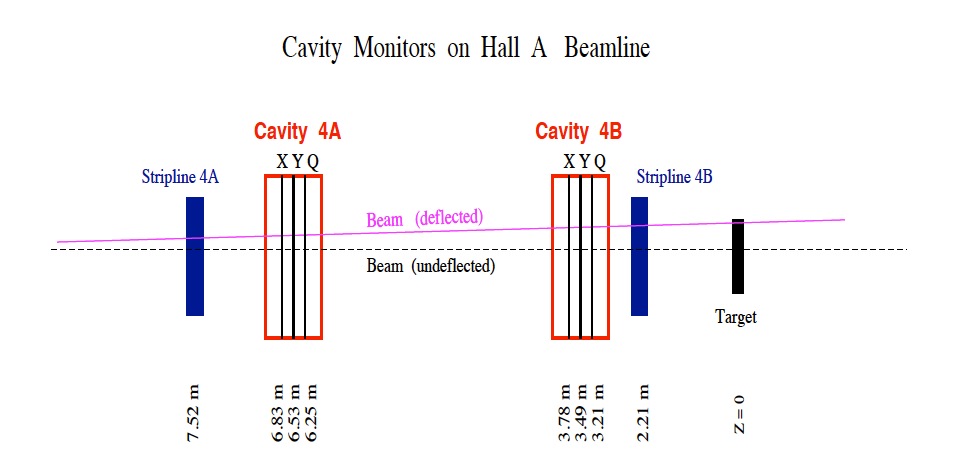
\includegraphics[width=0.49\linewidth]{bmw_modulated_beam}
% \end{figure}

%%%%%%%%%%%%%%%%%%%%%%%%%%%%%%%%%%%%%%%%%%%%%%%%%%%%%%%%%%%%%%%%%%%%%%%%
\section{Target}
For the sake of statistics, the designed current is quite large, as shown in
Table~\ref{tab:parameters}. With such high currents, the electron beam will deposit quite
a lot of heat on the target. It will be a disaster if the heat is not taken away 
as soon as possible, to keep a stable target temperature.
For PREX-II, because Pb itself is not a good thermal conductor ($\kappa = $35~W/(m$\cdot$K)),
auxiliary diamond foils ($\kappa >$ 1000~W/(m$\cdot$K)) are used to form a D-Pb-D 
sandwich target to help the heat dissipation. The thickness of the diamond foil matters, 
one lessen learned from PREX-I is that with a thin (0.15~mm) diamond foil, its
thermal conductivity dropped greatly (from 1000~W/(m$\cdot$K) to 100~W/(m$\cdot$K)) after about 
1 week of running with 70~$\mu$A cw beams, resulting in some Pb targets were melted. 
While a thicker diamond foil (0.25~mm) will protect Pb foils from melting 
under the same conditions. In PREX-II, a factor of 2 safety margin was adopted.
Conservatively assuming 1 week running for each Pb target, 35 days of beam time
requires 5 targets, and 10 isotopically pure Pb sandwich targets with thick 
diamond layers were deployed to ensure the success of PREX-II, each new target is able
to sustain up to 85~$\mu$A cw beams.

While Ca itself is an excellent thermal conductor ($\kappa =$ 200~W/(m$\cdot$K)), 
no need of auxiliary materials and higher current can be applied. 
The isotopically pure \Ca is much more expansive than the pure \Pb foil, so only 
one \Ca target (with a purity of 95.99\%) was prepared for CREX.
After the target accident, 
the new \Ca target was a stack of three separated foils with a similar total thickness
to the old one.
% https://logbooks.jlab.org/entry/3769028

Targets are firmly mounted in bays of target ladders, whose axes are 
perpendicular to the beam line. The ladder is movable along its axis by an 
alternating current (AC) servo motor, which can receive remote instructions 
through the internet. The motion along the ladder axis can be precise to 0.1~mm.
% prex2crex_target_paper_draft.pdf
% Thus each target foil would be placed at the same z position. 

There are 2 target ladders in total, one for production targets and the other
one for calibration targets. The production ladder has 16 target slots in total:
10 \Pb targets, two Calcium isotope targets -- \ca and \Ca, and four other 
calibration and diagnostic targets. The calibration ladder has only 5 targets:
a carbon hole, a watercell, a thin C foil, a thin natural Pb and a thin \ca target.
The production ladder is horizontal while the calibration ladder is rotated 
$45^\circ$ anti-clockwise w.r.t. the production ladder, 
as shown in Fig.~\ref{fig:scattering_chamber} and \ref{fig:target_ladder}.

\begin{figure}[!h]
    \centering
    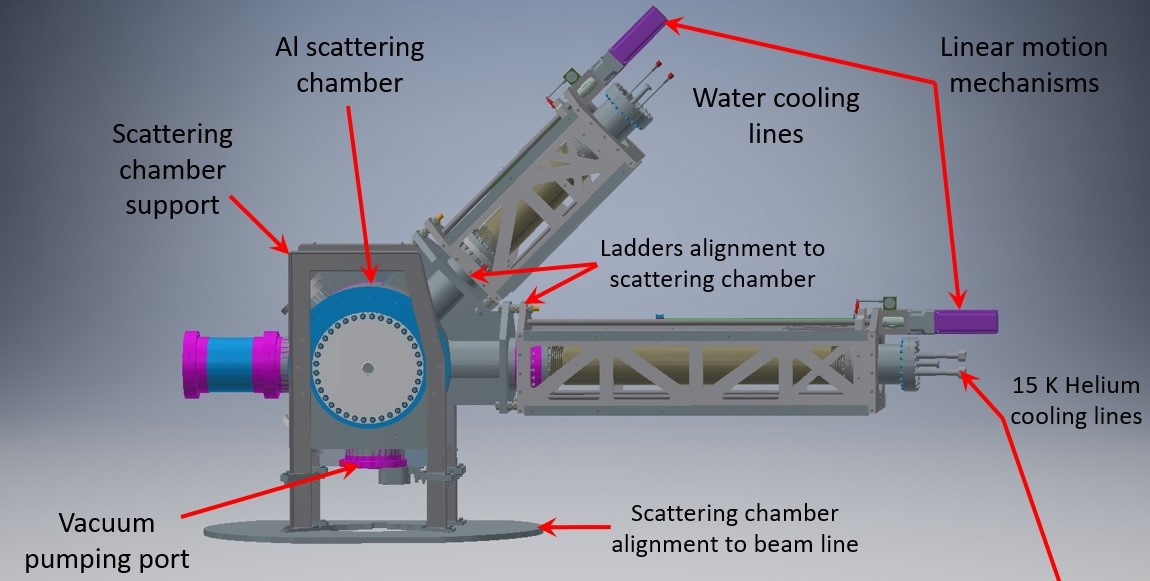
\includegraphics[width=\linewidth]{target_chamber}
    \caption{Design plot of the scattering chamber and the two target ladders.
    The horizontal one is the production ladder and the other one being the 
    calibration ladder.}
    \label{fig:scattering_chamber}
\end{figure}
\begin{figure}[!h]
    \centering
    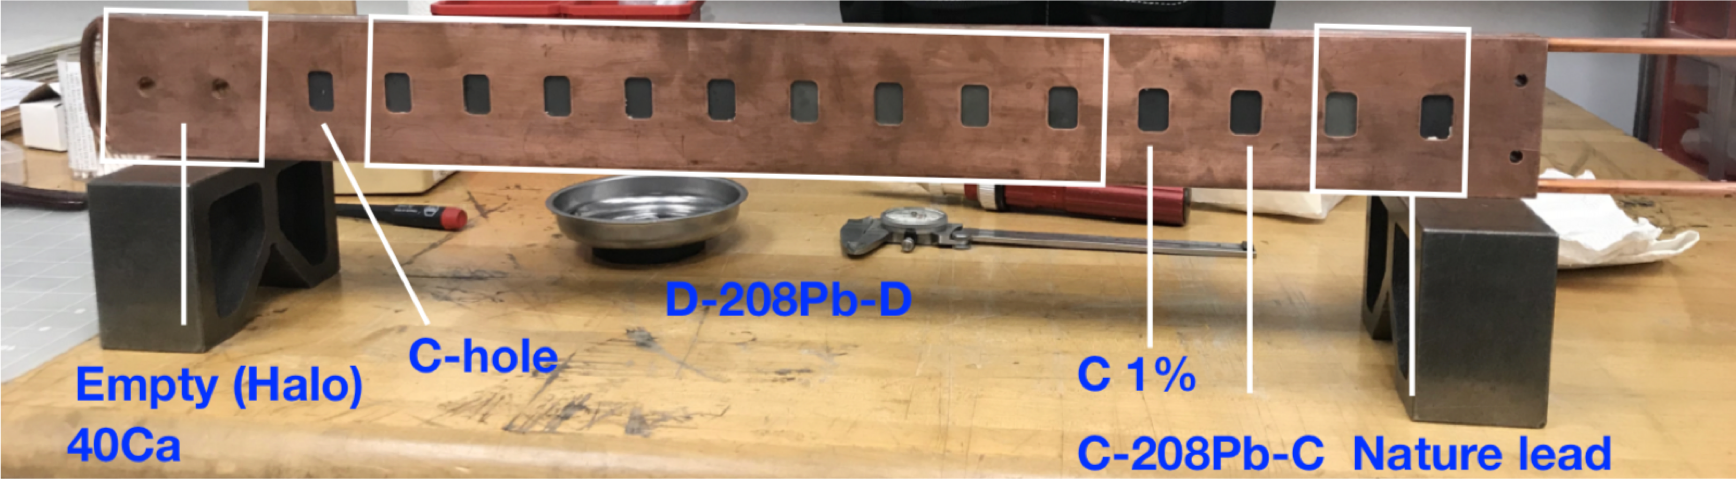
\includegraphics[width=0.67\linewidth]{target_ladder}
    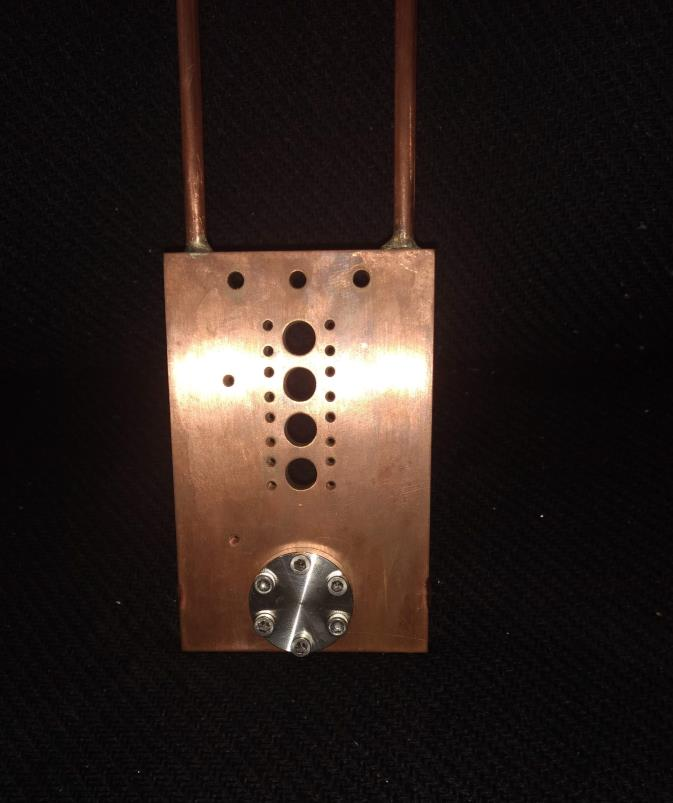
\includegraphics[width=0.2\linewidth, angle=90]{calibration_ladder}
    \caption{Actual pictures of the production (left) and calibration (right) ladders.}
    \label{fig:target_ladder}
\end{figure}

The \ca and \Ca targets are installed on the cold heat sink in dedicated cylindrical 
sockets at the end of the production ladder. % tilted $45^\circ$ to beam axis. 
The fact that the \Ca and the \Pb targets share the same ladder means they 
actually have the same z location, therefore the same scattering angle,
though they proposed different scattering angles ($5^\circ$/$4^\circ$ for PREX-II/CREX).
It being so to simplify the design, construction and installation of the target chamber.

Special care is needed for the \Ca target, the pressure should be less than $10^{-6}$~torr
to avoid the Ca oxidation. The vacuum of the target chamber is maintained by a 
turbo-molecular pumping system, which creates a $10^{-7}\ (10^{-8})$~torr vacuum 
for the calibration (production) ladder in the target chamber. When the beam is
not on, gate valves are closed to isolate the target chamber from upstream and 
downstream beam pipes. By way of precaution, a nitrogen purge system is 
installed to purge air in case of long term vacuum loss or the chamber needs
to be brought up to atmospheric pressure.
Every time we warmed up the \Ca target, gas boiling was needed before restarting 
the data taking.
% Ca oxidation: CaO, $\text{CaCO}_3$, $\text{Ca}_3\text{N}_2$, $\text{Ca(OH)}_2$

%%%%%%%%%%%%%%%%%%%%%%%%%%%%%%%%%%%%%%%%%%%%%%%%
\subsection{Target Cooling}
% allow for high luminosity
% we don't understand the failure modes of the target yet.
The production ladder is cryogenically cooled due to high power from electron beams,
while the calibration ladder is water cooled, the calibration runs need only
$\lesssim 1\ \mu$A level beam current. Both ladders are made of cooper.
The cooper frame of the production ladder is cooled by 15~K, 12~atm gaseous helium, 
which runs through the cooling tube surrounding the frame.
Contact between the target and the frame and within each layer of the \Pb sandwich
target are also important. Belleville washers are used to clamp the lead and 
diamond foils to ensure contact, besides, 
a thin layer of Apiezon L vacuum grease is applied to their interface to improve 
thermal conductivity. One hypothesis for the sudden failure of the Pb target after
one week of running is that the vacuum grease doesn't last long.
In the diamond/copper interface, a silver-based paste compound is used for the same purpose.
% https://prex.jlab.org/DocDB/0000/000012/001/tgtchamber_err2_17may2017.pdf
For a D-Pb-D sandwich target with a thick diamond foil, the heat loading will be $\sim$100~W\@70~$\mu$A
with a $4\times 6$~mm raster, the cooling system would keep the Pb target stay at
$\sim60$~K (melting point at $600$~K) assuming good contact and smooth heat
conduction. For the \Ca target, the $150\ \mu$A beam current will produce 
about 370~Watts heat on the target, which raised the target temperature 
up to $\sim300$~K (melting point at 1115~K).
% TargetOperation.pdf, tgtchamber_err2_17may2017.pdf


%%%%%%%%%%%%%%%%%%%%%%%%%%%%%%%%%%%%%%%%%%%%%%%%
\subsection{Raster}
Although the target foil was cooled to about 20~K (PREX-II), it still deformed (even melted)
under electron's bombardment. Small nonuniformities in the target 
thickness vary the scattering rate, and over the course of the experiment they 
eventually generated enough noise to swamp the tiny weak-scattering signal.
Actually, this is how we inspect the status of a target and evidence to
replace a target if the measured asymmetry width increase significantly.

\begin{figure}[!h]
    \centering
    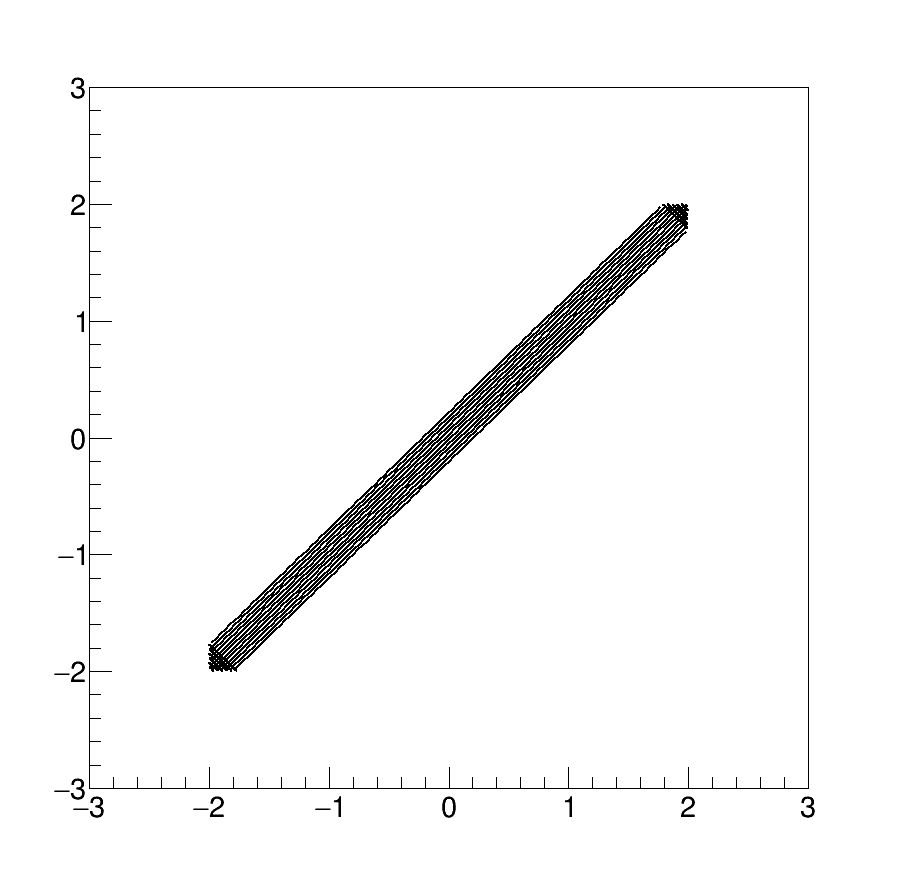
\includegraphics[width=0.48\linewidth]{raster_pattern_1}
    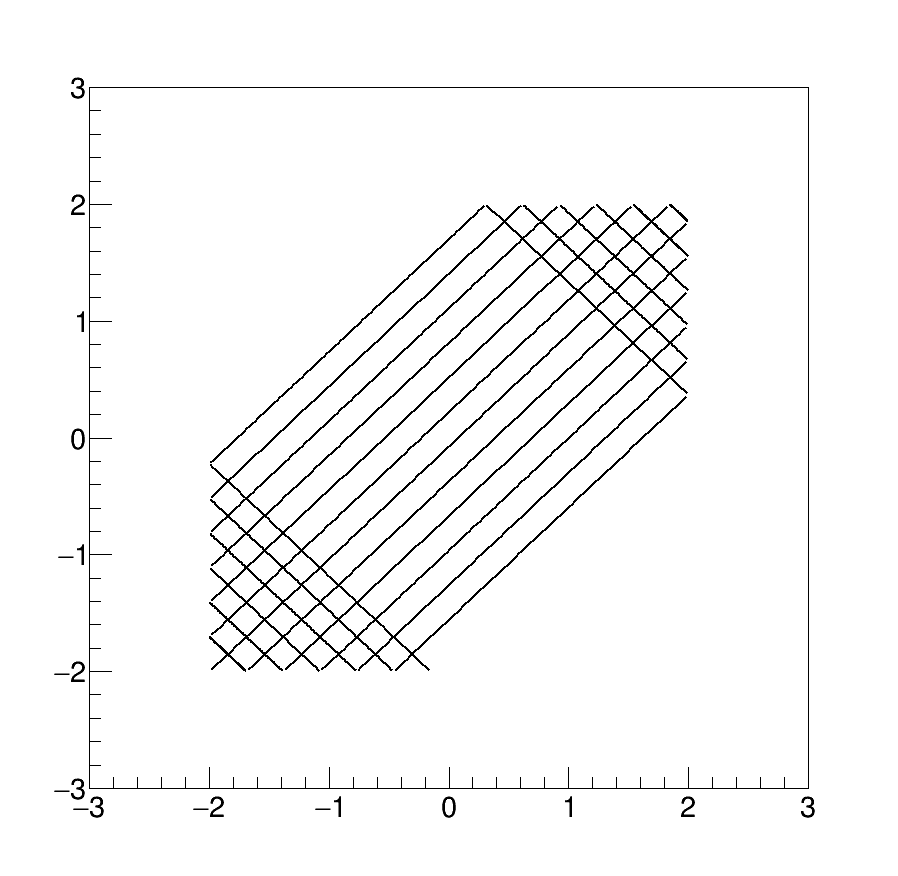
\includegraphics[width=0.48\linewidth]{raster_pattern_2}
    \caption{Raster pattern with different frequency difference between X and Y.
    Left: $|f_y - f_x| = 120\ Hz$; Right: $|f_y - f_x| = 8*120\ Hz$. The raster
    shape is a $4\times 4\ mm$ square.} 
    \label{fig:raster_pattern}
\end{figure}

The solution to this problem is the raster, which is a set of dipole magnets % where are they
between the Compton and the Moller polarimeters
that deflect the beam at about 25~kHz to spread the beam on the target.
What we learned from PREX-I was that we could significantly reduce the sensitivity 
to target-thickness variations by synchronizing the helicity flipping frequency
with the raster frequency so that it sampled exactly the same areas on the target,
any noise from target thickness variation cancels by taking the difference of
a helicity pair or quadruplet. 
As shown in Fig.~\ref{fig:raster_pattern}, the Lissajous pattern depends
on the frequency difference between X and Y, the larger the frequency difference,
the larger the scanning area. The ratio of $f_y/f_x$ should be an irrational number
to prevent a closed Lissajous pattern. The actual frequencies used were 25.44
and 24.48~kHz, for PREX-II, the raster size was $4 \times 6$~mm, and CREX
had a raster size of $2 \times 2$~mm.
% https://prex.jlab.org/wiki/index.php/Raster_Scope

\begin{figure}
    \begin{tikzpicture}
	\begin{scope}
	    \node[anchor=south west, inner sep=0] (image) at (0, 0)
	    { 
	    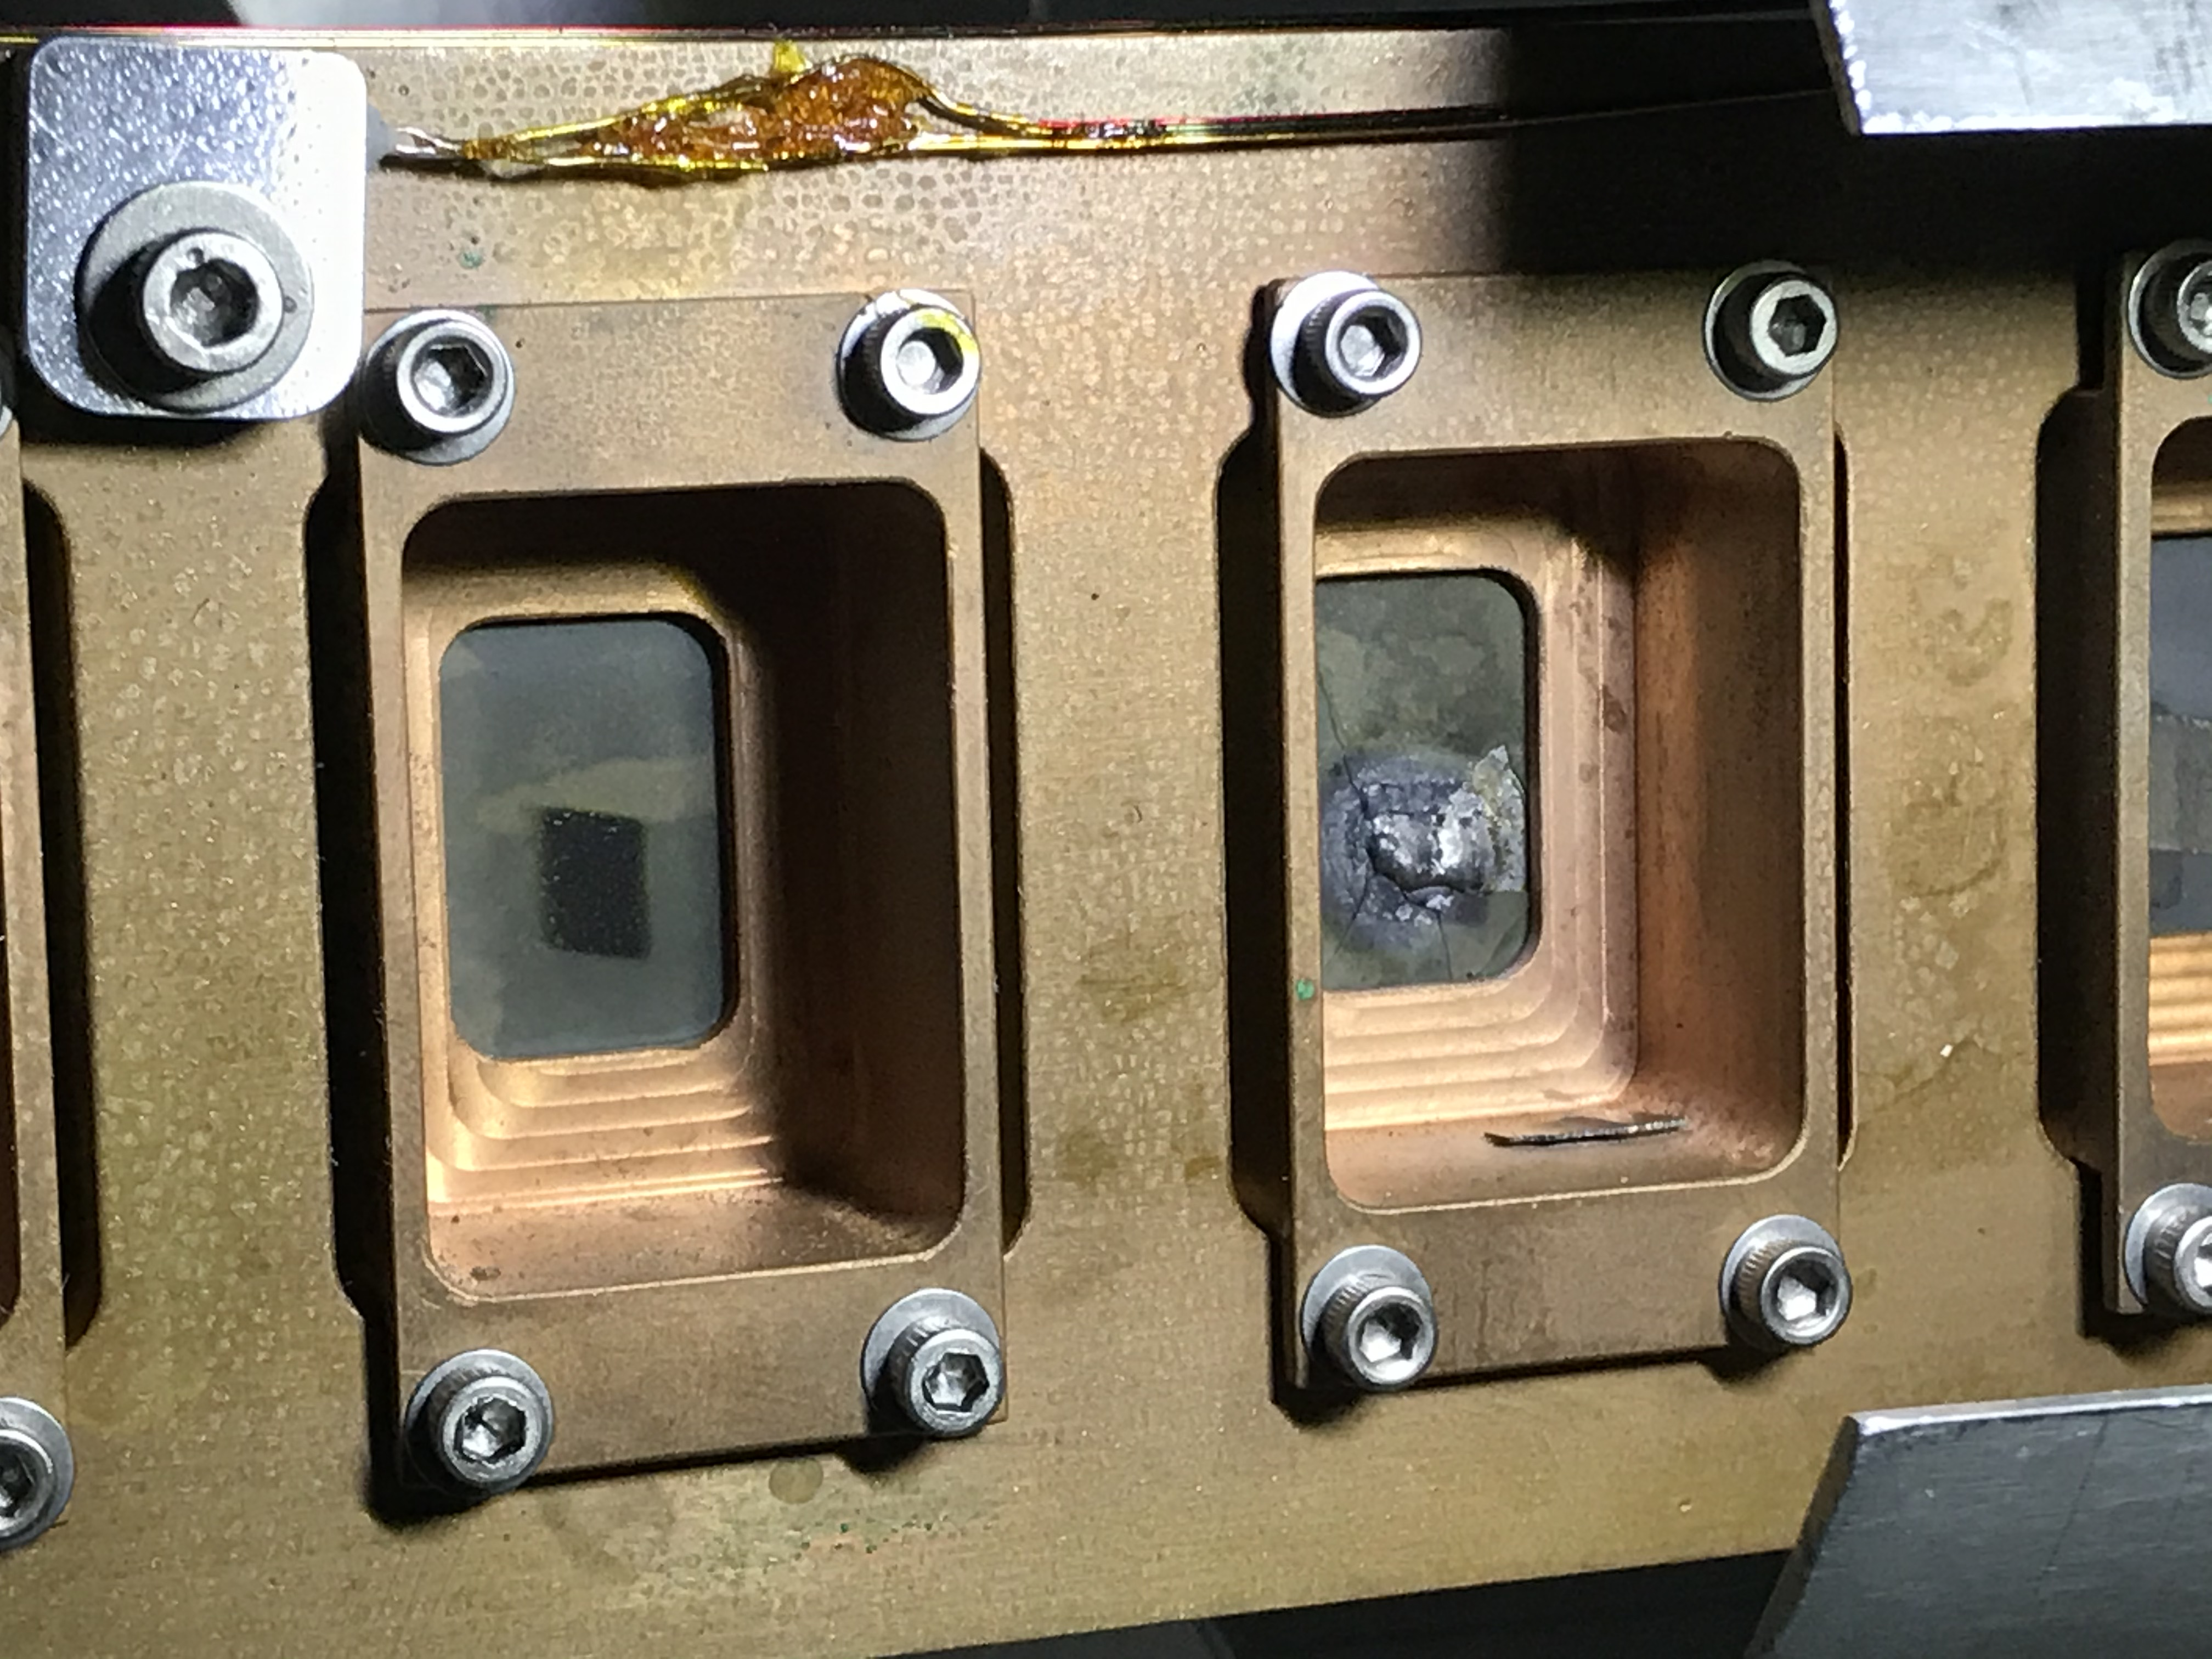
\includegraphics[width=0.32\linewidth]{prex_post_target_1}
	    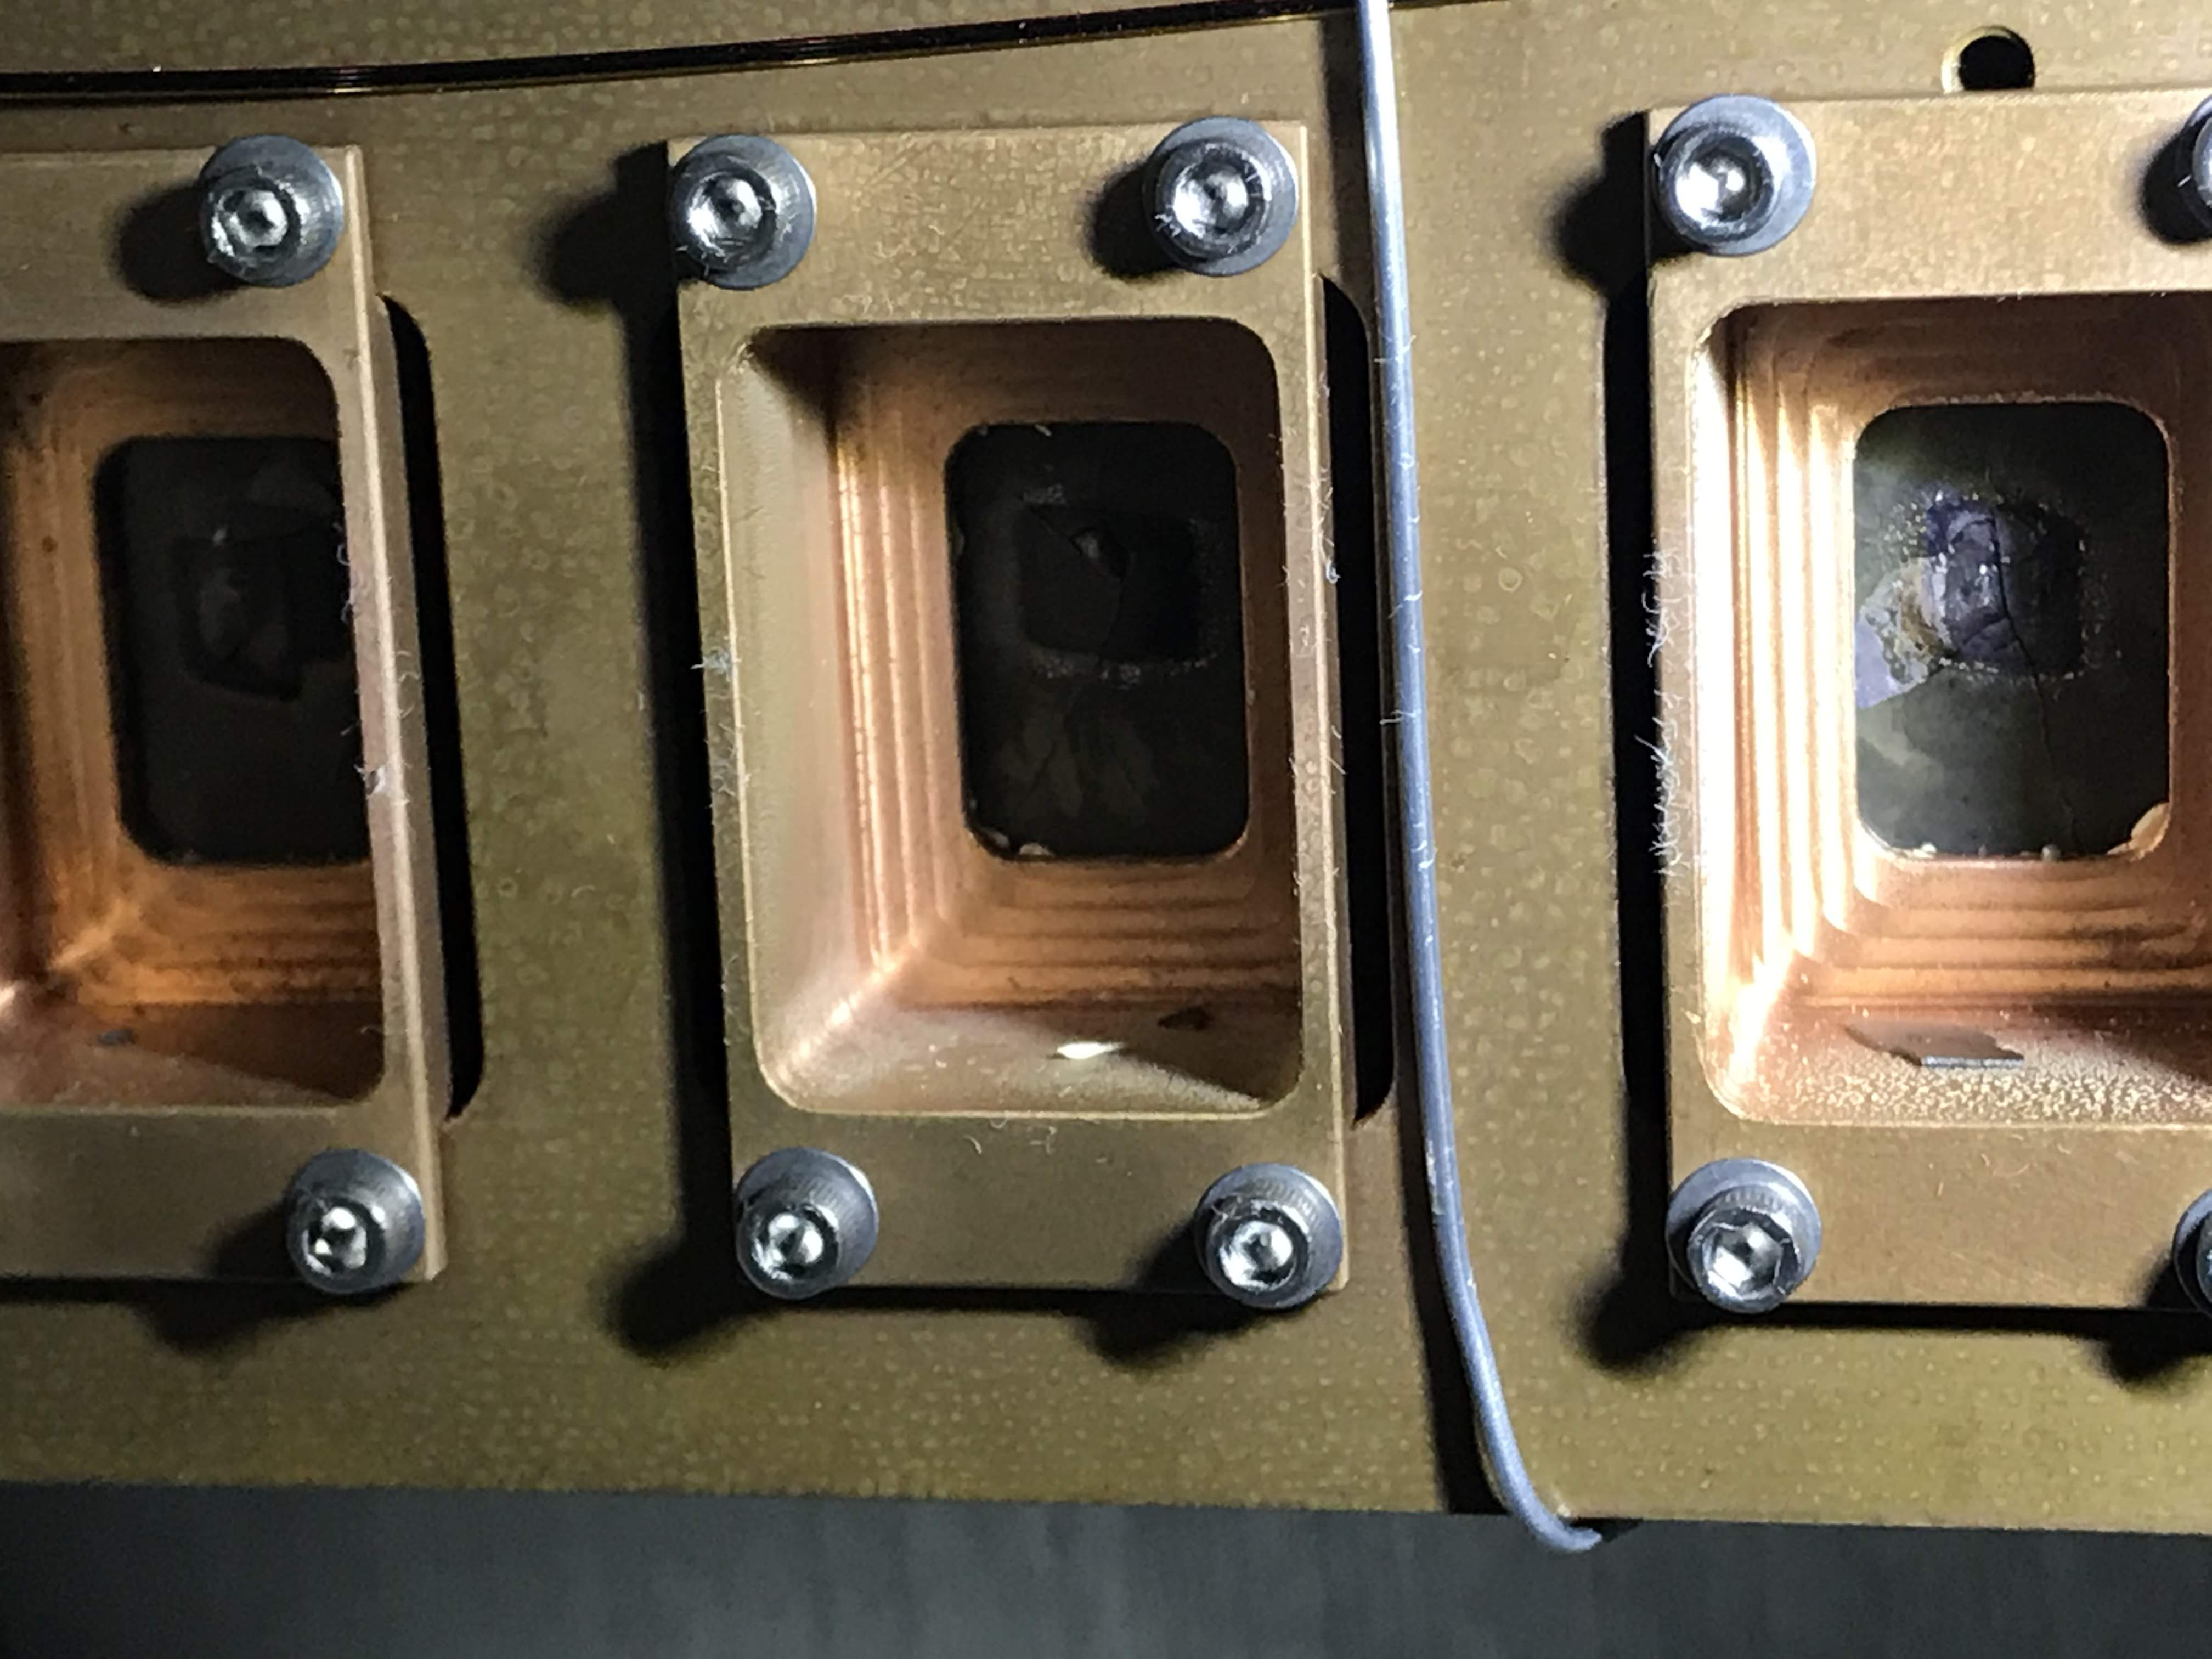
\includegraphics[width=0.32\linewidth]{prex_post_target_4}
	    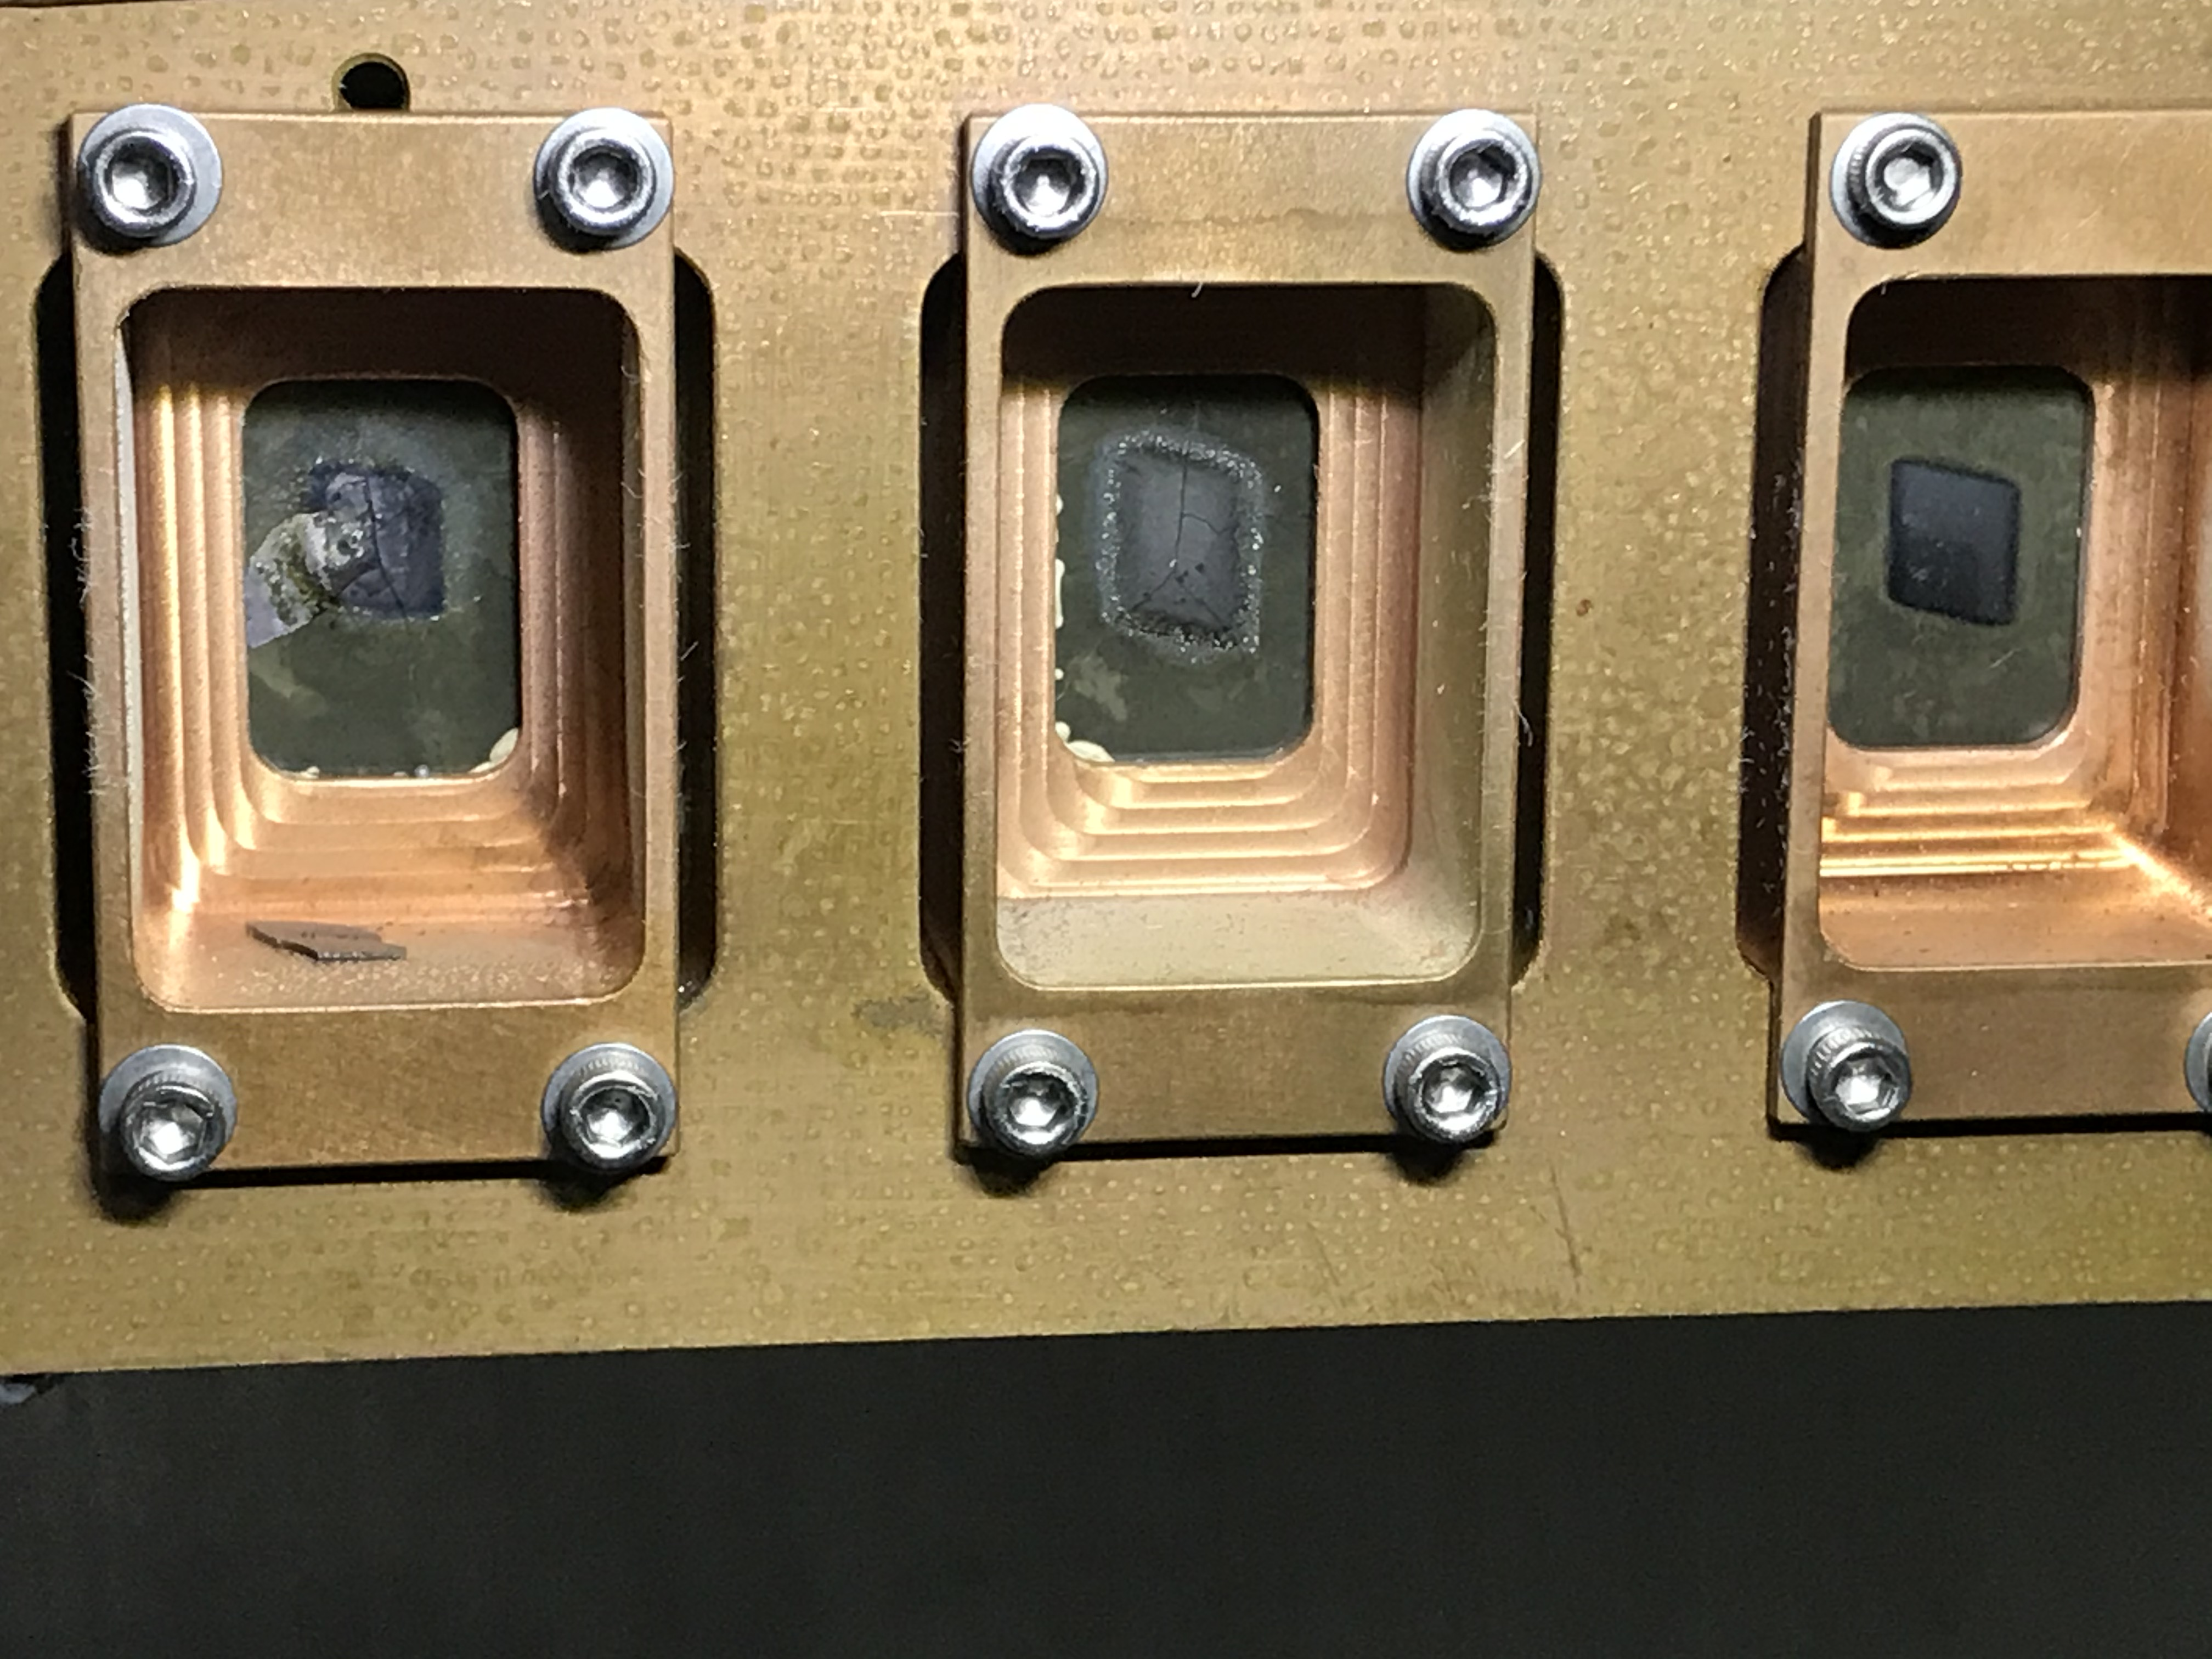
\includegraphics[width=0.32\linewidth]{prex_post_target_3}
	    };
	    \begin{scope}[x={(image.south east)}, y={(image.north west)}]
		\node [red] at (0.105, 0.19) {\textbf{Unused}};
		\node [red] at (0.235, 0.19) {\textbf{1}};
		\node [red] at (0.355, 0.22) {\textbf{2}};
		\node [red] at (0.49, 0.22) {\textbf{3}};
		\node [red] at (0.63, 0.22) {\textbf{4}};
		\node [red] at (0.73, 0.28) {\textbf{4}};
		\node [red] at (0.855, 0.28) {\textbf{6}};
		\node [red] at (0.975, 0.28) {\textbf{7}};
	    \end{scope}
	\end{scope}
    \end{tikzpicture}
    \caption{Picture of Pb targets after running, one can see clearly the shape
    of raster.}
\end{figure}

Another reason for having raster is heat dissipation, the larger the raster size,
the quicker the heat dissipation will be, the lower the target temperature, as
shown in Fig.~\ref{fig:target_temp_with_raster}.
\begin{figure}
    \centering
    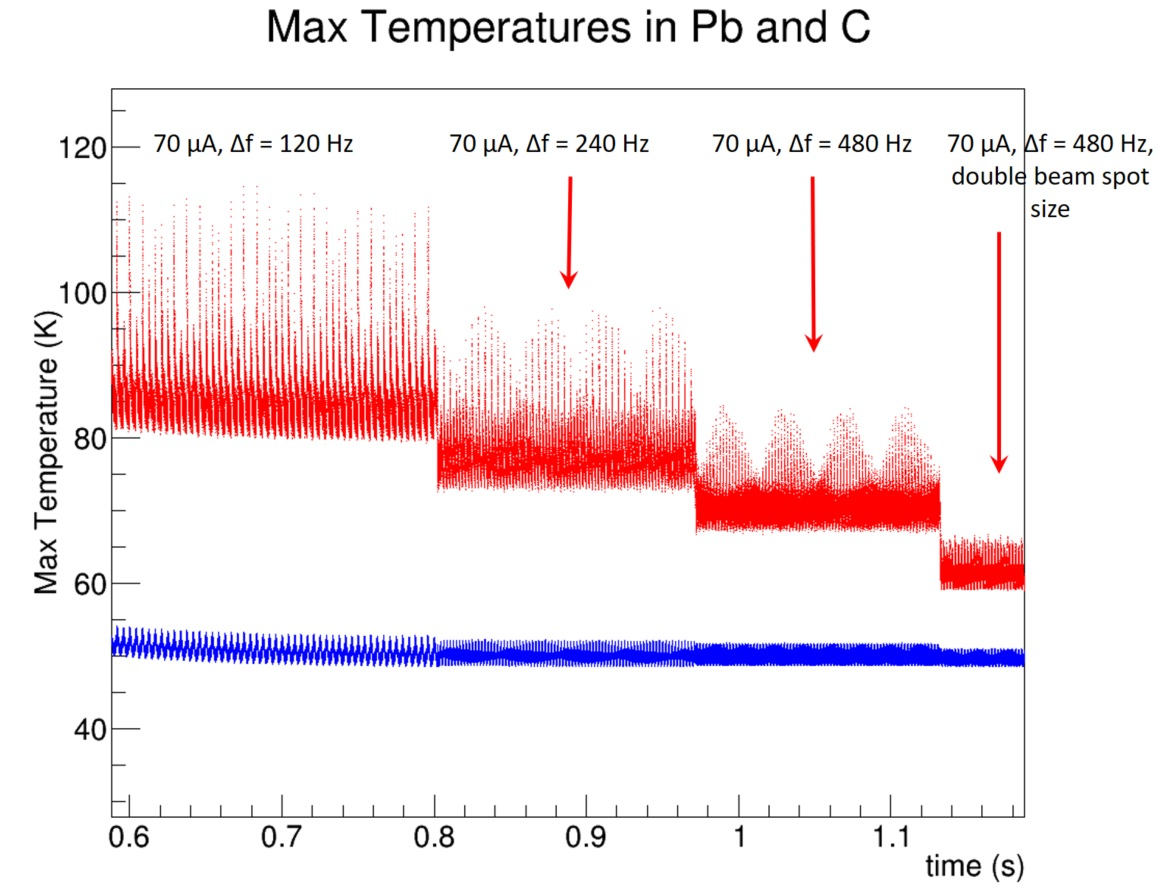
\includegraphics[width=0.5\linewidth]{target_temp_with_raster}
    \caption{How the target temperature change with size of raster area.}
    \label{fig:target_temp_with_raster}
\end{figure}

%%%%%%%%%%%%%%%%%%%%%%%%%%%%%%%%%%%%%%%%%%%%%%%%
\subsection{Beamline Collimator and Sieve Slit Collimators}
\begin{figure}[h!]
    \centering
    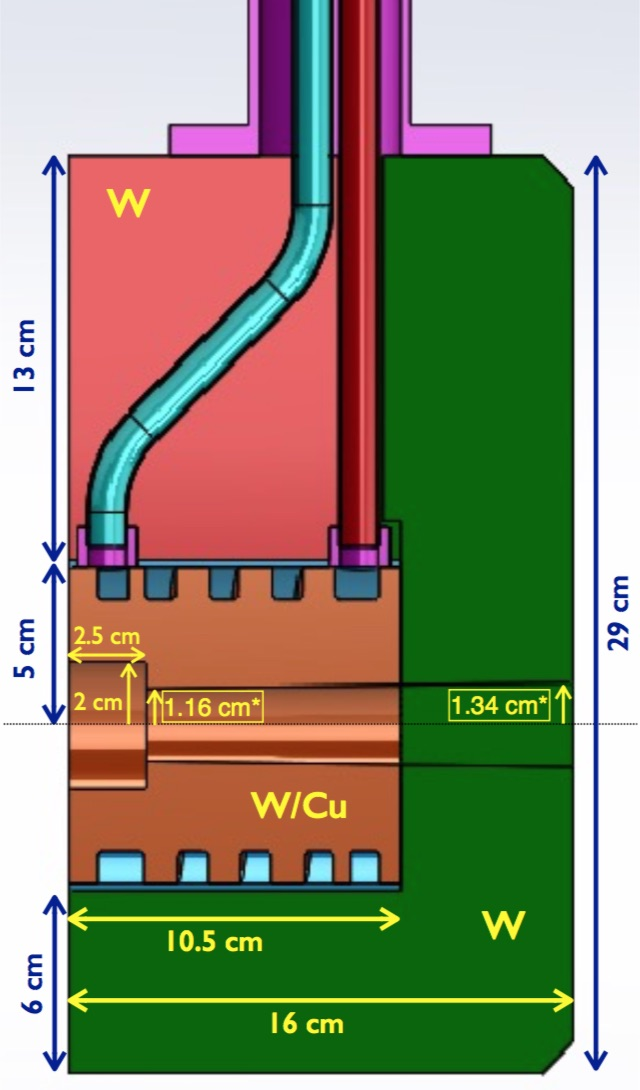
\includegraphics[height=0.21\paperheight]{beamline_collimator_side}
    \hspace{1 cm}
    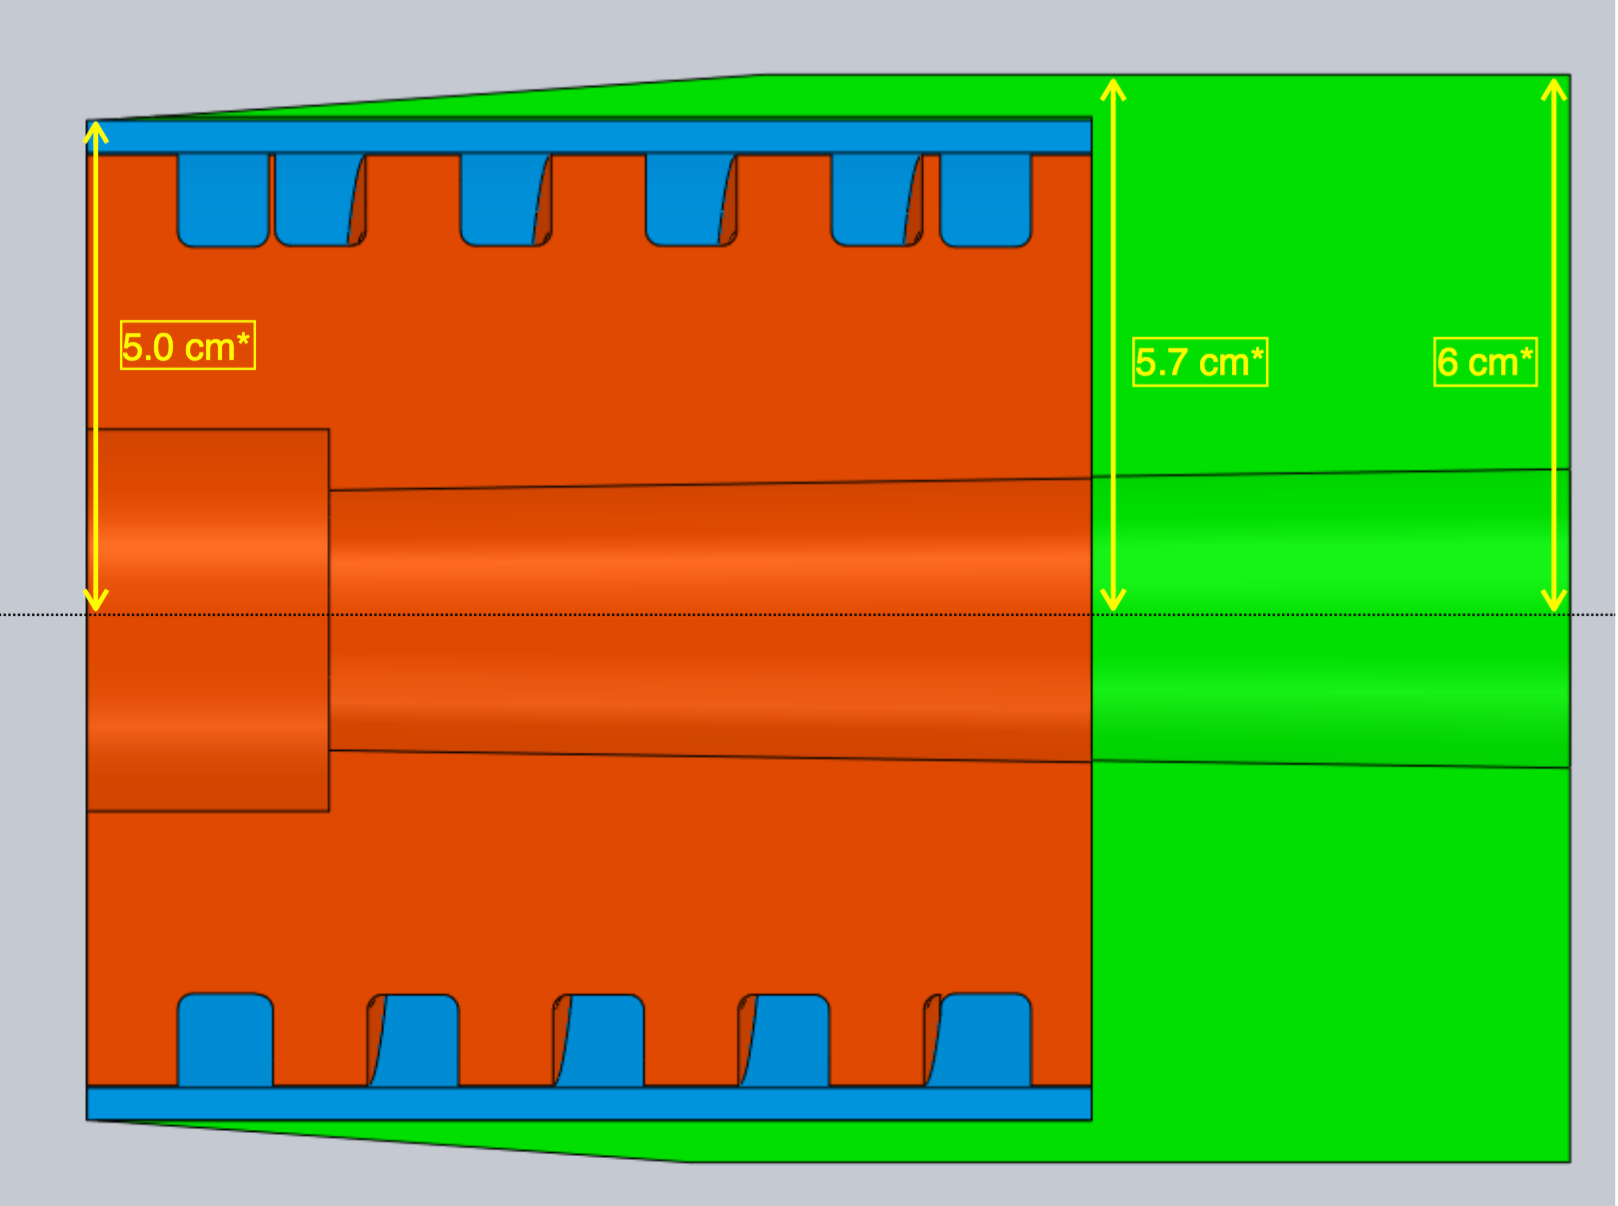
\includegraphics[width=0.4\linewidth]{beamline_collimator_top}
    \caption{Side and top view of beamline collimator. Beam from left to right.}
    \label{fig:beamline_collimator}
\end{figure}

Another problem that failed PREX-I was the excessive radiation, which damaged 
electronics in the Hall and the o-ring on the target exit flange leading to
leaks and ultimately halted the experiment.
% https://mailman.jlab.org/pipermail/halla_parity/2010-April/000197.html
With this experience, the new design of the pivot area (the center of the 2 HRS 
where the target chamber lies in) for PREX-II and CREX payed more attention
to radiation near the target region. The idea was to lead as much radiation to
beam dump as possible, and absorb the rest radiation in one key component --
the beamline collimator, which was placed $83\ cm$ downstream of the production 
target. The beamline collimator consists of an inner collimator and a housing
jacket made of sintered tunsgsten; the inner collimator, in turn, has the same 
structure of a 70\% W/30\% Cu alloy collimator and a copper jacket. As shown
in Fig.~\ref{fig:beamline_collimator}, there is cylinder notch in the front of
the inner collimator, to make sure the electrons/radiation are completely 
absorbed inside the collimator. The beamline collimator was water cooled, with
maximum heat loading of about $3.65\ kW$ from Pb target. The power on the beamline
% ffrom my simulation note
collimator was another signal for the degradation of target. When the temperature 
of the outgoing water increased dramatically, it was time to replace the target.
as shown in Fig.~\ref{fig:collimator_see_target_degradation}

Besides the beamline collimator, a few other devices were installed 
to further eliminate the radiation level in the hall. These devices include the 
high-density polyethylene (HDPE) neutron shield around the beamline collimator
region and a skyshine shield consisting of a $6\ cm$ thick tungsten block and
massive concrete blocks. These extra shields were used to block high energy
neutrons from the collimator.
% to make sure the site boundary does in a calendar year will not be exceeded.
% https://prex.jlab.org/DocDB/0000/000009/001/riordan_err_recommend-3.pdf

\begin{figure}[h!]
    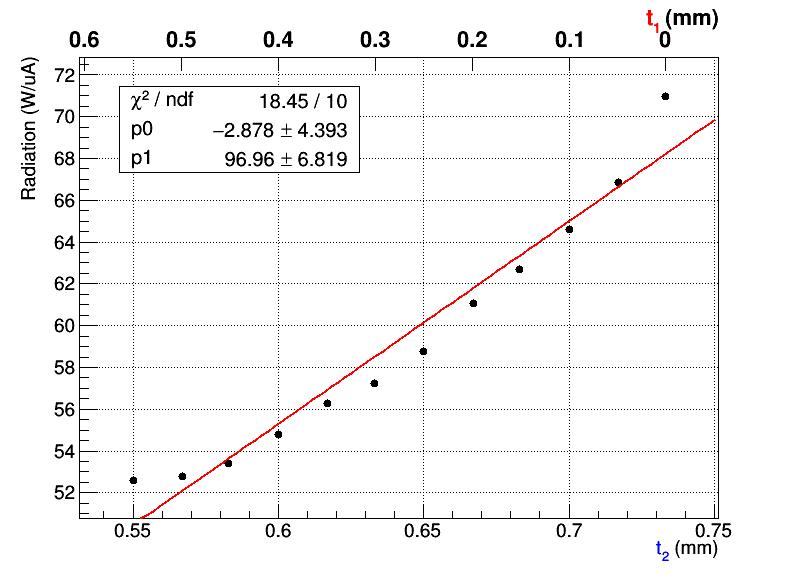
\includegraphics[width=0.32\linewidth]{collimator_power_fit}
    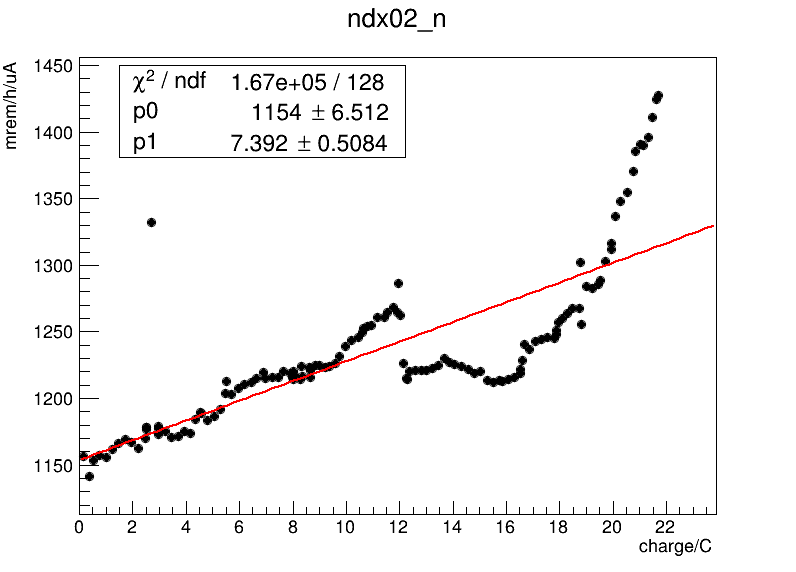
\includegraphics[width=0.32\linewidth]{Pb10_ndx02_n}
    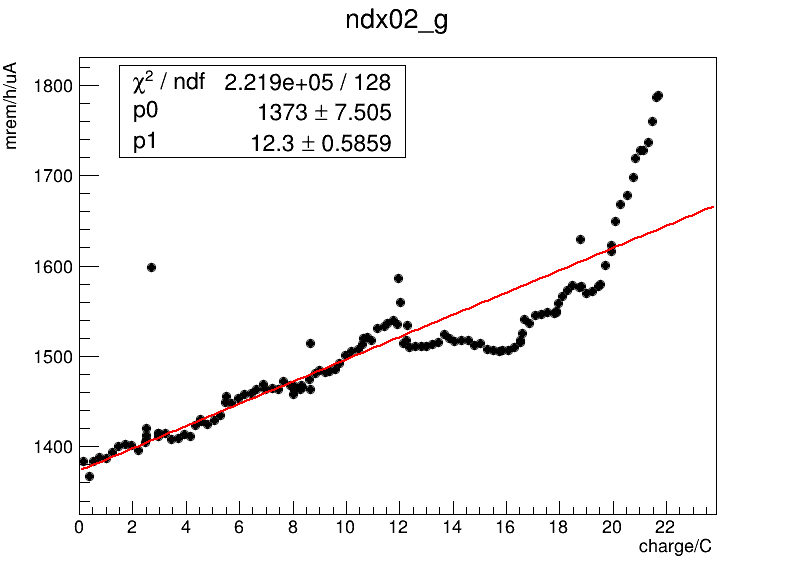
\includegraphics[width=0.32\linewidth]{Pb10_ndx02_g}
    \caption{Left: a simple model of target degradation -- assuming the inner 
    foil ($t_1$) is becoming thinner and the outer foil is becoming thicker ($t_2$) 
    while the total mass keeps intact. The plot shows how the power deposition 
    on the beamline collimator change in this model. Middle and Right: actual
    neutron and photon radiation level monitored along charge accumulation. They
    show similar trends.}
    \label{fig:collimator_see_target_degradation}
\end{figure}
% PREX-I O-ring failure: a large raster and a high current: 
% https://hallaweb.jlab.org/halog/html/1004_archive/100413092229.html

On both sides of the beamline collimator were the $5\ mm$ thick stainless steel
sieve slit collimators (about $1.1\ m$ from the target), which    % NIM paper
were used for optics study, helping electron trajectory reconstruction. When
we took production data, the sieve slit collimators were moved out of the spectrometer
acceptance; when we took optics data to measure the scattering angle and $Q^2$,
the sieve slit collimators were put in to cover the whole spectrometer acceptance,
without interfering the inner bore of the the beamline collimator. With known
(x, y) information of each hole in the sieve plane, together with the vertical
drift chamber (VDC) tracker, we can reconstruct the beam transport matrices.
\begin{figure}[h!]
    \centering
    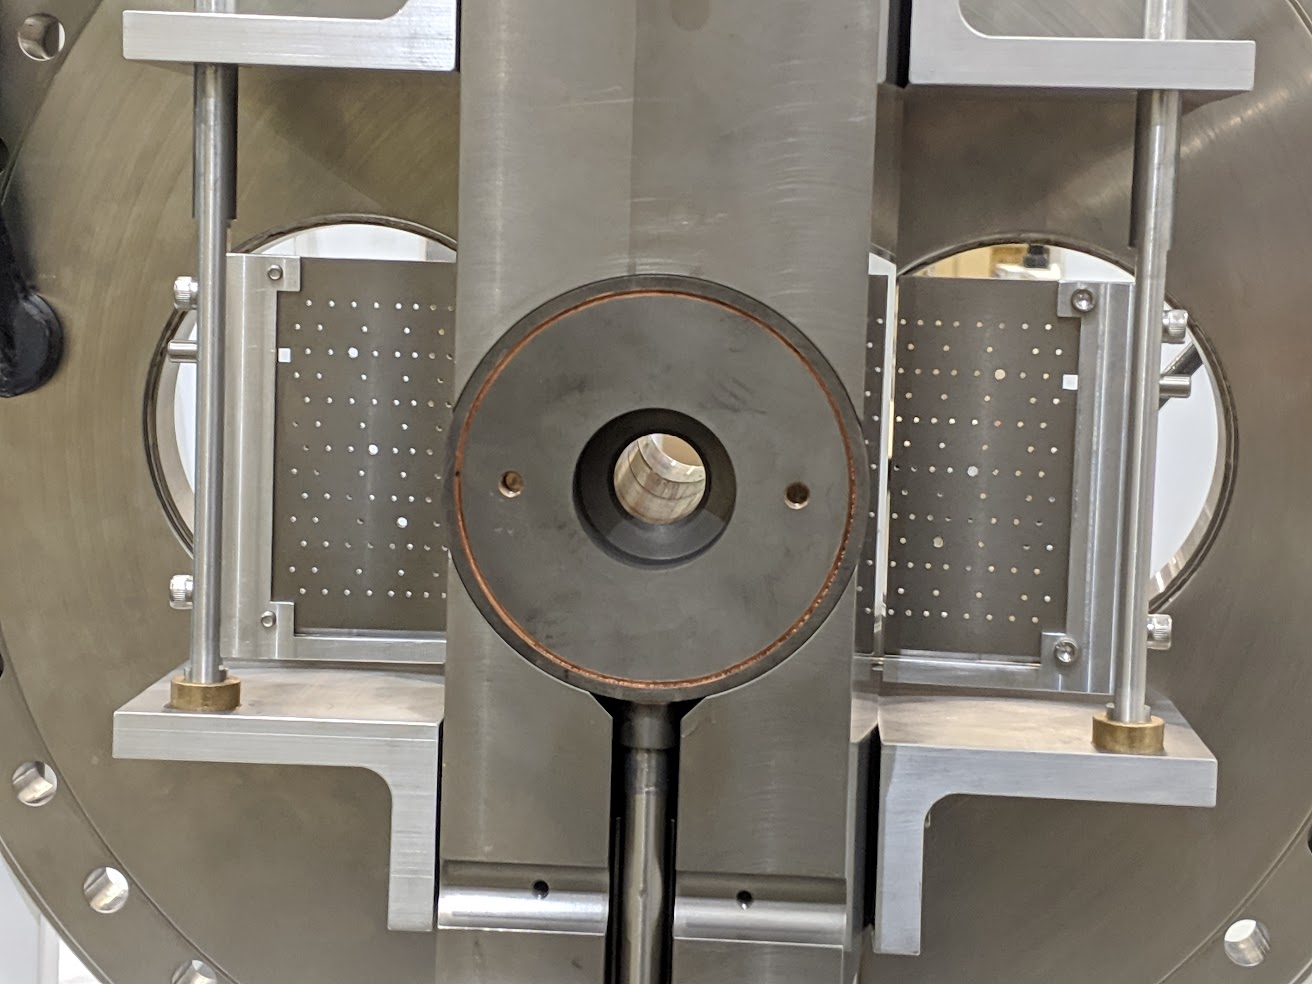
\includegraphics[width=0.48\linewidth, angle=180]{beamline_collimator_and_sieve_slit}
    \hspace{1cm}
    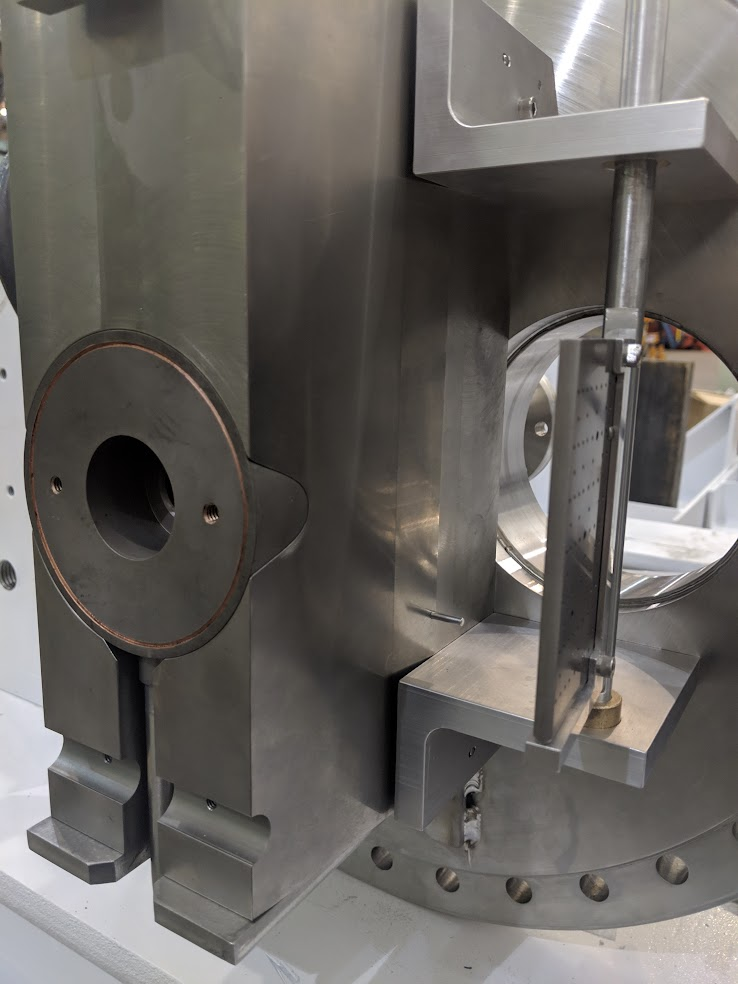
\includegraphics[scale=0.18, angle=180]{beamline_collimator_and_sieve_slit_1}
    \caption{Front picture of beamline collimator and sieve slit collimators, looking 
    downstream. One can clearly see a cylinder removed from the central collimator.
    The sieve planes lie after the beamline collimator and are movable like
    a door, it can be opened or closed remotely.}
\end{figure}

%%%%%%%%%%%%%%%%%%%%%%%%%%%%%%%%%%%%%%%%%%%%%%%%
\subsection{Septum}
The septum magnet is required to bridge the scattered electrons at small angle
into the HRS. As said before, the designed scattering angle is about $5^\circ$
while the smallest angle that HRS can reach is $12.5^\circ$, so a septum magnet 
is needed to guide the scattered electrons into HRS. 

The septum magnets are normal conducting magnets that consist of 3 coils, 
by applying large current, it will produce a
strong magnetic field (up to $\sim 1 \ T$ in the central region). A non-magnetic
stainless vacuum box will connect the upstream collimator box and the downstream 
HRS vacuum pipe on both sides of the septum. The septum beampipe (the one that
leads to the beam dump) is made of magnetic stainless steel to shield the
magnetic field from the septum, on both ends of the septum beampipe, there
are magnetic steel box to shield the fringe magnetic field from septum. 

% quad field resulted from the septum
\begin{figure}[h!]
    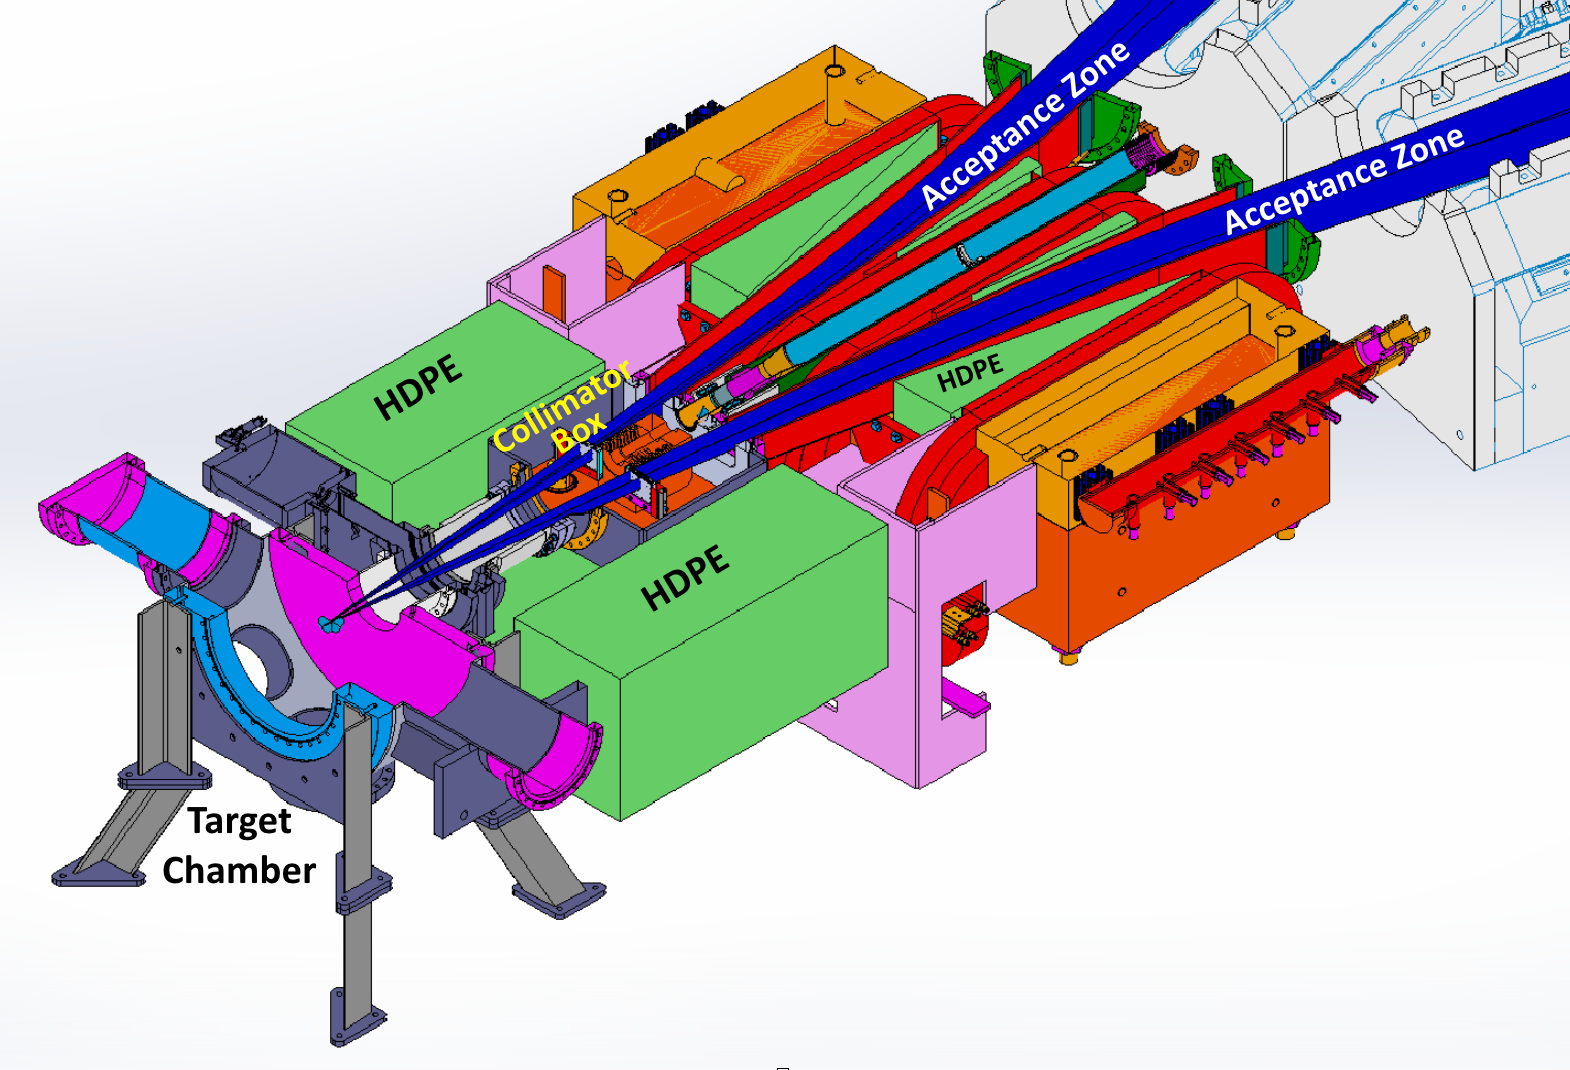
\includegraphics[width=0.52\linewidth]{septum}
    \includegraphics[width=0.46\linewidth]{septum_real}
    \caption{Left: septum (the red coils) in the pivot region; 
    Right: pciture of septum.}
\end{figure}

%%%%%%%%%%%%%%%%%%%%%%%%%%%%%%%%%%%%%%%%%%%%%%%%
\subsection{High Resolution Spectrometer (HRS)}
The key component of every Hall A experiment -- spectrometer. The most frequently
used ones are the high resolution spectrometer pair. Each HRS consists 3 superconducting
quadrupoles and 1 dipole. The maximum magnetic field of the 3 quadrupoles are
$1.2$, $1.0$ and $1.0\ T$ respectively while the dipole can provide up to $1.7\ T$ field. 
The incoming electrons will be bent $45^\circ$ up in the vertical plane and then
received by the following detectors.
HRS has a small angular acceptance ($\pm 28\ mr$ horizontally, $\pm 60\ mr$ vertically, 
% Vertical_drift_chambers_for_the_Hall_A_high-resolu.pdf
the solid angle being $7.8\ msr$), but can move over a wide range of angle
around the hall ($12.5^\circ - 165^\circ$). As its name implies, it achieves a 
very high momentum resolution at the $10^{-4}$ level over a wide range of momentum 
($0.8 - 4\ GeV$). This capacity helps to reject most of inelastic electrons, 
because a small difference in electron momentum ($2-3\ MeV$) will lead to
large separation in the detector plane, thus leaving us a relative clean data 
with very small background from inelastic scattering. 

\begin{figure}[h!]
    \centering
    \includegraphics[width=0.32\linewidth]{HRS_1}
    \includegraphics[width=0.32\linewidth]{hrs_rays}
    \includegraphics[width=0.32\linewidth]{hrs_inelastic}
    \caption{Schematic plot of HRS and particle rays inside it. \cite{halla3d}
    The 'focal plane' in the middle plot, by design, should be at an angle of $45^\circ$
    w.r.t the central ray, but is actually rotated to $70^\circ$ due to lackness
    of sextupole winding in Q3. When we talk about the HRS focal plane, we
    usually refer to the VDC lower plane.
    }
\end{figure}

% HRS magnetic field were monitor by 2 arrays of 3 NMR field probes	% NIM paper

Before the entrance of Q1 quadrupoles was the Q1 collimator, which defined
the spectrometer acceptance. It was strictly required that the symmetry between
left/right, and up/down of Q1 collimators should be preserved to reduce any
possible systematic uncertainties.
\begin{figure}[h!]
    \centering
    \includegraphics[width=0.5\linewidth]{Q1_collimator}
    \caption{Picture of Q1 collimator pairs}
\end{figure}
%%%%%%%%%%%%%%%%%%%%%%%%%%%%%%%%%%%%%%%%%%%%%%%%
\subsection{Detector Package}
The standard HRS detector package on each arm consists of trigger scintillators for
triggering, a pair of VDCs for particle tracking, Cherenkov type detectors and
shower counters (calorimeters) for particle identification (PID). In PREX-II
and CREX, only parts of these detectors are needed, namely VDCs and S0/S3 triggers,
others were removed for safety. We built our own Cherenkov counters that can 
work in the so called 'intergrating mode'.
\begin{figure}[h!]
    \centering
    \includegraphics[width=0.5\linewidth]{detectors_1}
    \caption{The detector package}
    \label{fig:detectors}
\end{figure}

\subsubsection{Vertical Drift Chamber (VDC)}
Each VDC detector package consists of 2 drift chambers, one lower and one upper
chamber with a vertical separation of $0.23\ m$ ($0.335\ m$ between the same
U or V planes of the lower and upper chamber), to enable precise position and angle measurement. 
The drift chamber is actually a multiwire proportional chamber (MWPC) with 2 
layers of sense wires -- U and V planes in the lab horizontal plane, which are 
orthogonal to each other and has a vertical separation of $26\ mm$. 
Each wire plane consists of 368 tungsten wires with the width of adjacent wires 
being $4.24\ mm$, corresponding to $6\ mm$ in the spectrometer cross section due to the $45^\circ$
cross angle between the central ray and the VDC plane. The ion's drift time in 
the chamber are used to reconstruct particle trajectory. The single plane can
achieve a position resolution of $\sim 235\ mm$ FWHM, the angular resolution
is $6\ mrad$ FWHM for $\theta$ (out-of-plane angle) $2.3\ mrad$ for $\phi$ (in-plane
angle) \cite{FISSUM2001108}.
% composition, configuration and performance
\begin{figure}[h!]
    \centering
    \includegraphics[width=0.5\linewidth]{VDC}
    \caption{Schematic plot of VDCs showing UV wires \cite{FISSUM2001108}}
\end{figure}

VDCs were only used for optics runs in PREX-II and CREX, when we collect electrons
one by one to measure their scattering angle and energy, otherwise they were
turned off during normal production runs.

% VDC efficiency: http://ace.phys.virginia.edu/HAPPEX/4463

%%%%%%%%%%%%%%%%%%%%%%%%
% \subsubsection{GEMs}

%%%%%%%%%%%%%%%%%%%%%%%%
\subsubsection{Trigger}
Same as VDCs, triggers were only used in counting mode for optics study. The standard
detector package consists of multiple trigger planes, only 2 of them were used :
the S0 and S3 plastic scintillators. The S0 scintillator locates between VDCs and the main
detectors while S3 lies behind the main detectors, they have a sensitive area
of $170\ cm$ long by $25\ cm$ wide. Their signals were logically combined to 
provide different trigger rate. The trigger rate was controlled to be less
than $50\ kHz$ most of the time (the up limit of VDC is about $250\ kHz$).
% T1 records 8.4 kHz for 1.5 uA
%%%%%%%%%%%%%%%%%%%%%%%%
\subsubsection{Main Detector}
The main detector of PREX-II and CREX was the $5\ mm$ thick fused silica (quartz) tiles,
with a size of $16\ cm$ long by $3.5\ cm$ wide ($3\ cm \times 3\ cm$ active area). 
2 identical quartz detectors were installed with the upstream one used as the 
main detector and the downstream one as the backup (also used for a cross check 
in PREX-II). They are tilted to be perpendicular to the electron rays.
The high refractive index of quartz ($n\approx 1.45$) means the opening angle $\theta$
in Fig.~\ref{fig:quartz} is about $46^\circ$, larger than the critical angle
to make total internal reflection ($\theta_c = \arcsin\frac{1}{n} = 43.6^\circ$),
therefore, the Cherenkov light produced by high energy electrons will be totally
reflected inside the quartz and finally collected by the PMT. The high photon
yield make it easier to resolve the electron peak, which was beneficial given
the fact that non-linearity of the PMTs is one of the major contributors to 
systematic uncertainties.
\begin{figure}
    \includegraphics[width=0.3\linewidth]{quartz}
    \includegraphics[width=0.3\linewidth]{Cherenkov}
    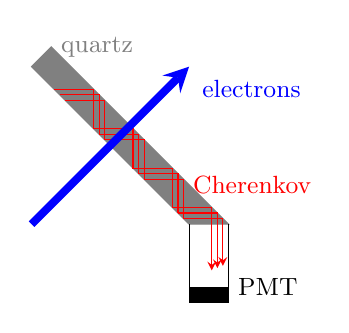
\begin{tikzpicture}[xshift=2cm]
	\draw[fill, Gray] (0, 0) -- ++(-2,2) -- ++(0.25, 0.25) node[right] {\small{quartz}} -- ++(2.25, -2.25) -- (0, 0);
	\draw (0, 0) -- ++(0, -0.8) -- ++(0.5, 0) node[right] {\small{PMT}} -- ++(0, 0.8);
	\draw[fill] (0, -0.8) -- ++(0, -0.2) -- ++(0.5, 0) -- ++(0, 0.2);
	\foreach \i in {1, 2, 3}{
	    \draw[red] (135:\i*0.1) -- ++(0, 0.5) -- ++(-0.5, 0) 
		-- ++(0, 0.5) -- ++(-0.5, 0)
		-- ++(0, 0.5) -- ++(-0.5, 0);
	    \draw[red, -stealth] (135:\i*0.1) -- ++(0.5, 0) -- ++(0, -0.5-\i*0.1);
	    }
	\draw[-stealth,Blue, line width=1mm] (-2, 0) -- ++(2, 2) node[below right] {\small{electrons}};
	\node[red] at (0.8, 0.5) {\small{Cherenkov}};
    \end{tikzpicture}
    \caption{Left: CAD drawing of the quartz detector; 
    Middle: schematic plot of Cherenkov radiation, the angle between 
    electron and the Cherenkov radiation is 
    $\cos\theta = \frac{v_c}{v_e} = \frac{c}{nv_e} = \frac{1}{n\beta} \approx \frac{1}{n}$;
    Right: electron flux goes through a quartz detector.
    }
    \label{fig:quartz}
\end{figure}

\begin{figure}
    \centering
    \includegraphics[width=0.5\linewidth]{quartz_QE}
    \caption{Simulation result of photo-electron (PE) spectrum for single electron
    passing through the main detectors. The wider tail in the downstream
    detector is due to particle showering in the upstream quartz.
    Plot from Devi Adhikari.}
\end{figure}
The width of the photon-electron distribution will increase
the statistical uncertainty:
\begin{equation}
    \sigma_{A} = \sigma_{stat} \times \sqrt{1 + \left( \frac{\sigma_{PE}}{\langle PE \rangle }\right)^2}
\end{equation}
where $\sigma_{PE}$ is the RMS of the distribution. The RMS can be parameterized
into 2 parts: the Gaussian principle part which is inversely proportional to
the quartz thickness and a Landau tail which comes from the showering process
and is proportional the thickness. The final decision of $5\ mm$ of thickness
was a compromise between these 2 parts to minimize detector resolution 
$\frac{\sigma_{PE}}{\langle PE \rangle}$: thicker to increase photon-electron
yield and thinner to reduce showering.

\begin{figure}
    \centering
    \includegraphics[width=0.32\linewidth]{quartz_x}
    \includegraphics[width=0.32\linewidth]{quartz_y}
    \includegraphics[width=0.32\linewidth]{quartz_xy}
    \caption{Data of x,y distribution on quartz. Plots from Devi Adhikari.}
\end{figure}

There was a homemade motion control system in each arm to move the main detectors
remotely, which allowed us to tune the position of the main detectors when we
changed gain of the main detectors under a different beam current.

% Can we used it as calorimeter? How do measure the beam energy?

%%%%%%%%%%%%%%%%%%%%%%%%
\subsubsection{AT Monitors}
% last page of https://prex.jlab.org/DocDB/0000/000096/002/riordan_prex_soft.pdf
About $1\ m$ downstream the main detector were a pair of AT monitors, as shown 
in Fig.~\ref{fig:detectors}, which used exactly the same quartz piece as the 
main detectors. They were used to monitor transverse polarization in the beam.
\begin{figure}[h!]
    \centering
    \includegraphics[width=0.48\linewidth]{ATL1}
    \includegraphics[width=0.48\linewidth]{ATL2}
    \caption{Scatter plot of electrons on the AT monitor plane. Red and blue represent
    events with opposite transverse polarization. 
    % Some dots outside the AT acceptance due to showering in the upstream main detectors
    }
\end{figure}

%%%%%%%%%%%%%%%%%%%%%%%%%%%%%%%%%%%%%%%%%%%%%%%%
\subsection{Data AcQuisition (DAQ)}
JLab has its own framework of hardwares and softwares to aquire data, which
is called CODA (CEBAF Online Data Acquisition) \cite{CODA}. It is a distributed
system that can be scaled from a few detector channels to tens of thousands of
channels needed in an experiment. CODA version 2.6.2 was used for PREX-II and CREX.
% CODA data structure: https://hallaweb.jlab.org/equipment/daq/dstruct.html

Data acquisition worked in 2 modes: the integrating mode and the counting mode,
both have their own DAQs, because they had different triggers and read from
different detectors.

%%%%%%%%%%%%%%%%%%%%%%%%
\subsubsection{Integrating DAQ}
The integrating DAQ consists of 4 primary DAQ systems spread in the injector,
the Counting House (CH) and the hall (LHRS/RHRS). They are controlled by the
CODA Run Control system in the CH, and triggered by the helicity signal.

The helicity signal was produced by a Helicity Control Board \cite{Hboard} 
located in the Injector Service Building, which is an Advanced Programmable Logic
Generator. It has 4 timing modes: 3 fixed-frequencies of 30, 120 and 240~Hz
and a fourth free-running mode. In fixed-frequency mode, as we chose in PREX-II/CREX,
the phase was locked to the `Beam Sync': the accelerator's 60~Hz AC line synchronized 
global timing reference, which means the last helicity window in a helicity pattern
may be shorter or longer than other helicity windows because the 60~Hz line signal
wanders from time to time, shown as Beam Sync Jitter in the second timing diagram 
in Fig.~\ref{fig:timing}. To ensure that all helicity windows have the same integrating
time, an artificial deadtime was introduce, which was $T_{\text{dead}} = 51.33 \mu$s,
as shown in Fig.~\ref{fig:integrating_timing}.
This slightly reduce the integration time: $T_{\text{int}} = T_{\text{stable}} - T_{\text{dead}}$.
% Beam sync signal: SCAM module, https://prex.jlab.org/wiki/index.php/Helicity_Control

\begin{figure}
    \centering
    \includegraphics[width=0.9\linewidth]{timing}
    \caption{Helicity timing diagram. The Tsettle signal (falling edge) indicates 
    the start of a new helicity window, which was chosen as the t=0 reference
    point for all timing diagram, it goes to the CH/hall.
    The QRT (Pattern Sync) signal indicates the start of each helicity pattern,
    it goes to the CH. 
    The Pair Sync signal toggles between 0 and 1, indicating the start and end
    of a helicity pair, it goes to the CH. This signal is not important, all it
    tells can be inferred from the QRT signal.
    The Hel+ signal decides the helicity of the current window, it goes to the 
    laser table in the injector.
    The Hel- signal is a complementary signal to Hel+, so that the board always 
    keeps the same current regardless of the helicity state, preventing helicity 
    correlated electrical pickup from the board. This signal is not shown in the
    plot, it goes to the helicity magnets (Wien filters).
    The Delayed Helicity (DLY RPT) signal (by specified n windows).
    It tells what the helicity was n windows before. It goes to the CH. This
    signal is not shown in the plot.}
    \label{fig:timing}
\end{figure}

The helicity signal sent to injector components (PCs, IAs and the Wien Filters) 
can be regarded as real time due to their geographical vicinity. The Tsettle 
signal sent to hall A 
will stop (falling edge) data taking in the previous helicity window, then hold for
$T_{\text{settle}}$ time to allow settlement of the high voltage in PCs % $0\ \mu s$
and readout of previous window data, its rising edge tells the start time of data taking in current 
helicity window. The delay caused by signal transportation in fiber optics cables to Hall A 
was about 100~ns, 1~$\mu$s was reserved between the Tsettle and the helicity
signals to inform the hall of the change of helicity, as shown in Fig.~\ref{fig:timing}.
Actually, this is not necessary, because $T_{\text{settle}} = 90\ \mu$s was long enough to
allow such delay in signal transportation, as well as delay caused by beam 
transportation in the accelerator, which was $1.4 \text{km/c} = 4.7\ \mu$s.

The actual helicity signal (DLY RPT) sent to Hall A will be delayed (by 8 helicity windows
in PREX-II/CREX), so that no monitors along the beamline or detectors in the 
hall know the helicity of current window, making sure that the monitors/detectors
were not helicity sensitive. In the DAQ side, we needed to verify that
the helicity pattern is expected based on the helicity pattern signal and the 
measured helicity agrees with the delayed helicity signal, to ensure that the
helicity information was correct. When doing data analysis, the data needs 
to be shifted number of delayed helicity windows to match the actual helicity 
pattern. The helicity pattern was pseudo-randomly chosen by the helicity board 
using a 30-bit Shift Register.

% https://prex.jlab.org/DocDB/0001/000187/001/PREX_DAQ_25July18.pdf
The analog signals from the main detectors and various beam monitors were converted 
to voltage by a customised I-to-V 
pre-amplifier developed for the Qweak experiment, the voltage output was fed
to a 18-bit ADC (Analog-Digital-Converter), sampled and integrated there. The
18-bit ADC was also a product of previous parity experiments. The detector signal was
sampled every $2\ \mu$s and integrated into 4 sub-blocks for each helicity window
(1024 samples per sub-block, 4096 samples per helicity window at 120~Hz).
The ADC will be triggered $80\ \mu$s after the start of $T_{\text{settle}}$, as shown
in Fig.~\ref{fig:integrating_timing}, this allows $10\ \mu$s wait time for 
ADC to void any possible effects from the external triggering NIM pulse on the 
internal signal processing. To synchronize data collection (integration), 
a HAPPEX Timing Board (HAPTB) was used, which received the Tsettle signal and
produced the integration gate signal, distributing them to each ADC/scalar to trigger
signal integration/collection.
% HAPTB: https://prex.jlab.org/wiki/index.php/DAQ_Hardware_HAPTB

\begin{figure}
    \centering
    \includegraphics[width=\linewidth]{integrating_timing}
    \caption{Integrating timing}
    \label{fig:integrating_timing}
\end{figure}

Each DAQ has its own VME crate holding all necessary hardware modules, a read 
out controller (ROC) controls the VME crate. All these crates (ROCs) were
managed by a Trigger Supervisor (TS), which had its own VME crate. The TS was
triggered by the Tsettle signal, which in turn trigger the ROCs.
By receiving the triggering signal, ROC will read data stored in their memory 
buffer and send it to the CODA system, 
which will build, transport and store events. We had an analyzer JAPAN (Just
Another Parity ANalyzer) to monitor online data and analyze data off-line.

% \begin{figure}
%     \centering
%     \includegraphics[width=0.5\linewidth]{Coda}
% \end{figure}

%%%%%%%%%%%%%%%%%%%%%%%%
\subsubsection{Counting DAQ}
The 2 counting DAQs, one for each HRS, were different from the integrating DAQs,
in both hardwares and softwares. In contrast to counting electrons in the integrating
mode, the counting DAQ record and recounstruct track for each scattered electrons.
The counting DAQ read data from the scintillators,
VDCs and GEMs, the main detectors were not used in the counting DAQ; and was
triggered by the scintillators, different logical combinations of the scintillator
signals could trigger different counting rates. Most of the time, we used the S0
trigger signal, as discussed in the scintillator sector.

The analyser used for decoding counting mode data was the general Hall A analyser,
which will read out the hit information in each detector and reconstruct the 
electron track based on these hits. By reversing the optics matrix, it will
calculate the electron info (position, angle and energy) on the target, allowing
to measure the scattering angle and $Q^2$, to tune the optics matrix, 
to do detector alignment and check backgrounds.

%%%%%%%%%%%%%%%%%%%%%%%%
\subsubsection{EPICS}
Besides the two DAQ systems, there is a site-wise slow (relative to the helicity frequency) 
control system, called Experimental Physics and Industrial Control System (EPICS) \cite{EPICS},
to monitor and control every important apparatus and quantity, such as magnets, 
beam current/position/energy, vacuum level, temperature, gas flow, 
high voltage supply etc. EPICS polled a series of 
Input/Output Controllers (IOCs) and record their average values about every second.
It provides real-time monitoring of the whole system: both accelerator and detectors, and
allows us to trace back the status whenever there were some problems.
